% \documentclass[letterpaper,11pt]{article}
% \documentclass[twocolumn]{article}
\documentclass{article}

% \usepackage{multicol}
\usepackage[margin=1.57in]{geometry}  %Default is 1.75in for 11pt

\usepackage[utf8]{inputenc}
\usepackage[english]{babel}

\usepackage{amsmath}            % improve math presentation
\usepackage{graphicx}           % takes care of graphic including machinery
\usepackage[hyphens]{url}       % URL typesetting; need [hyphens] so long URLs go to next line (instead of margins)
\usepackage[final]{hyperref}    % adds hyper links inside the generated pdf file
\hypersetup{
	colorlinks=true,            % false: boxed links; true: colored links
	linkcolor=blue,             % color of internal links
	citecolor=blue,             % color of links to bibliography
	filecolor=magenta,          % color of file links
	urlcolor=blue
}
\usepackage[blocks]{authblk}    % authors and \affill
\usepackage{color}
\usepackage{soul}               % highlight text \hl{}

\usepackage[font=small,labelfont=bf, textfont=it]{caption}  % Figure captioning: small font, Figure is bolded, text is italics

% Pretty quotes: https://tex.stackexchange.com/questions/53377/inspirational-quote-at-start-of-chapter
\definecolor{quotemark}{gray}{0.7}
\makeatletter
\def\fquote{%
    \@ifnextchar[{\fquote@i}{\fquote@i[]}%]
           }%
\def\fquote@i[#1]{%
    \def\tempa{#1}%
    \@ifnextchar[{\fquote@ii}{\fquote@ii[]}%]
                 }%
\def\fquote@ii[#1]{%
    \def\tempb{#1}%
    \@ifnextchar[{\fquote@iii}{\fquote@iii[]}%]
                      }%
\def\fquote@iii[#1]{%
    \def\tempc{#1}%
    \vspace{1em}%
    \noindent%
    \begin{list}{}{%
         \setlength{\leftmargin}{0.1\textwidth}%
         \setlength{\rightmargin}{0.1\textwidth}%
                  }%
         \item[]%
         \begin{picture}(0,0)%
         \put(-15,-5){\makebox(0,0){\scalebox{3}{\textcolor{quotemark}{``}}}}%
         \end{picture}%
         \begingroup\itshape}%
 %%%%********************************************************************
 \def\endfquote{%
 \endgroup\par%
 \makebox[0pt][l]{%
 \hspace{0.8\textwidth}%
 \begin{picture}(0,0)(0,0)%
 \put(15,15){\makebox(0,0){%
 \scalebox{3}{\color{quotemark}''}}}%
 \end{picture}}%
 \ifx\tempa\empty%
 \else%
    \ifx\tempc\empty%
       \hfill\rule{100pt}{0.5pt}\\\mbox{}\hfill\tempa,\ \emph{\tempb}%
   \else%
       \hfill\rule{100pt}{0.5pt}\\\mbox{}\hfill\tempa,\ \emph{\tempb},\ \tempc%
   \fi\fi\par%
   \vspace{0.5em}%
 \end{list}%
 }%
 \makeatother
 
%======================== Title & Abstract =========================
\begin{document}

\title{Is the Internet Green?}
\author[1]{\textbf{Stephanie Knill} \\ sknill@cs.toronto.edu \\ 1006179181}
\affil[1]{Department of Computer Science, The University of Toronto}
\date{\today}

\renewenvironment{abstract}
 {\quotation\small\noindent\rule{\linewidth}{.5pt}\par\smallskip
  {\centering\bfseries\abstractname\par}\medskip}
 {\par\noindent\rule{\linewidth}{.5pt}\endquotation}

\maketitle
\begin{abstract}
\noindent Is the Internet green? Contrary to the image portrayed by the high technology and innovation sector, Internet and communication technology (ICT) are physical entities that leave a footprint on our planet. With over half of the world population using the Internet and the continuing proliferation of ICT devices, this question is becoming increasingly urgent. Using the life cycle assessment (LCA) to assess the potential environmental impacts and resource consumption, we will follow each life stage of an ICT device from the cradle to the grave: raw material acquisition, manufacturing, distribution, usage and end-of-life. 
% Metals compromise a sizeable portion of ICT devices and so we examine the environmental consequences of the mining process (from prospecting to reclamation), as well as the challenges associated with extracting rare earth elements and the geopolitical implications of critical, scarce and conflict minerals. 
Lastly we will discuss some of the systemic unintended consequences triggered by the widespread ICT infrastructure and devices, including surveillance capitalism and social media as a tool for social movements.

\end{abstract}

%%%%%%%%%%%%%%%%%%%%%%%%%%%%%%%%%%%%%%%%%%%%%%%%%%%%%%%%%%%%%%%%%%%%%%%%
%%%%%%%%%%%%%%%%%%%%%%%%%%% 3 Minute Thesis %%%%%%%%%%%%%%%%%%%%%%%%%%%%
%%%%%%%%%%%%%%%%%%%%%%%%%%%%%%%%%%%%%%%%%%%%%%%%%%%%%%%%%%%%%%%%%%%%%%%%
% \cleardoublepage
% \section{3 Minute Thesis}
% Is the internet green? Contrary to the image portrayed by the high technology and innovation sector, internet and communication technology (or ICT) are physical entities that leave a footprint on our planet. With over half of the world population using the internet and the continuing proliferation of ICT devices in our lives, this question is becoming increasingly urgent. For my research, I am using the life cycle assessment to examine the potential environmental impacts and resource consumption of our ICT devices. This approach examines the ecological footprint of our ICT devices at each stage of its life, from the cradle to the grave.

% In the first stage, we need to \textbf{acquire the raw materials} necessary to produce our devices. These typically comprise of plastics, glass and an assortment of metals---silver, gold, tin, tantalum and the rare earth elements to name a few. In addition to the regular environmental tolls of mining, rare earth elements typically hitch-hike with radioactive elements, therefore causing radioactive waste and radioactive contamination around the mining sites and surrounding neighbourhoods. Each of the conflict minerals (known as the 3TG -- tin, tungsten, tantalum and gold) are required to produce a single smartphone and as we discussed in class there is much work to be done to ensure an equitable resource governance in Africa. The next stage is the \textbf{manufacturing} process; here lies the majority of the emissions in a typical ICT device due to the extensive processing required to obtain a high purity of silicone for our processor chips. Next we have the \textbf{distribution} phase, where goods are packaged and transported either to stores or directly to customers. The \textbf{usage} phase represents the energy required to power our devices and the internet infrastructure and the ease at which your devices are able to be repaired and reused. At the \textbf{end of an ICT device's life}, it becomes e-waste. About 18\% of e-waste is recycled; the fate of the remaining 82\% is unknown. For the lucky devices that do get recycled, the plastics can only be downcycled into lower grade uses while many of the metals have very poor recycling rates (for example, all of the REE have a $<$ 1\% recycling rate). Waste colonialism is especially prevalent: developed nations use their dominance to exploit the land of developing nations for their waste disposal. Due to the high cost of regulations in the formal recycling sector, it is more economical for developed countries to load their wastes onto ships and trains, transport them beyond their regulated jurisdictions and dump them onto a developing nation's land for a fee. This massive transboundary movement of e-waste onto developing nations has resulted in them bearing the brunt of the damage generated from e-waste dumping and recycling.

% In addition to a more traditional LCA, I also examined the systemic unintended consequences triggered by this widespread adoption of ICT devices and infrastructure. These include the sharing (or gig) economy, mental health, and the rise of surveillance capitalism as a dominant economic model. 

%%%%%%%%%%%%%%%%%%%%%%%%%%%%%%%%%%%%%%%%%%%%%%%%%%%%%%%%%%%%%%%%%%%%%%%%
%%%%%%%%%%%%%%%%%%%%%%%%%%% Table of Contents %%%%%%%%%%%%%%%%%%%%%%%%%%
%%%%%%%%%%%%%%%%%%%%%%%%%%%%%%%%%%%%%%%%%%%%%%%%%%%%%%%%%%%%%%%%%%%%%%%%
\cleardoublepage
{\hypersetup{linkcolor=black}  % Make hyperlinks in table black (instead of blue)
\tableofcontents}

%%%%%%%%%%%%%%%%%%%%%%%%%%%%%%%%%%%%%%%%%%%%%%%%%%%%%%%%%%%%%%%%%%%%%%%%
%%%%%%%%%%%%%%%%%%%%%%%%%%%%%% Background %%%%%%%%%%%%%%%%%%%%%%%%%%%%%%
%%%%%%%%%%%%%%%%%%%%%%%%%%%%%%%%%%%%%%%%%%%%%%%%%%%%%%%%%%%%%%%%%%%%%%%%
\cleardoublepage
\section{Background} \label{SECTION_BACKGROUND}
 \begin{fquote}[John Naughton][The Internet: Everything you ever need to know \cite{naughton2010internet}] The internet has quietly infiltrated our lives, and yet we seem to be remarkably unreflective about it. That's not because we're short of information about the network; on the contrary, we're awash with the stuff. It's just that we don't know what it all means. We're in the state once described by that great scholar of cyberspace, Manuel Castells, as ``informed bewilderment".
 \end{fquote}

%%%%%%%%%%%%%%%%%%%%%%%%%%%%%%%%%%%%%%%%%%%%%%%%%%%%%%%%%%%%%%%%%%%%%%%%
%%%%%%%%%%%%%%%%%%%% Physicality of the Internet %%%%%%%%%%%%%%%%%%%%%%%
\subsection{The Physicality of the Internet}
Internet and communication technology (ICT) are the devices, networking components, applications and systems that combine to allow people and organisations to interact in the digital world \cite{techtarget2020ICT}. While the list of ICT components is continually growing, it can be broadly categorized into 

\begin{itemize}
    \item \textbf{Hardware}: the physical technology that works with information. Some examples include smartphones, computers and smart fridges.
    \item \textbf{Software}: a set of instructions that tells the hardware what to do. This is often further subdivided into system software (operating systems such as Windows or iOS that manage the hardware's operation) and application software (handling spreadsheets, social media, games)
    \item \textbf{Transactions}: some examples of this include online shopping, telemedicine, and online banking
    \item \textbf{Communication Technology}: connects the hardware together to form a network. This connection can be through wire (ethernet cables or fibre optics) or wireless (wifi)
    \item \textbf{Data}: the information that the other components work with resides. In a database, data is collected and it can be retrieved by querying it. On a larger scale, data warehouses contain all of the data in whichever form that an organization needs.
    \item \textbf{Internet Access}
    \item \textbf{Cloud Computing}: on-demand computer system resources (especially data storage and computing power) accessible to users over the Internet \cite{hayes2008cloud}
\end{itemize}

Contrary to what the name suggests, the cloud is in the ocean---it is on the bottom of the sea floor, going through deep sea trenches and reefs \cite{starosielski2012warning, blum2012tubes}. Since the late 1970s, more than 4 billion km of silica fibers have been laid across the world (the distance from Earth to Neptune) \cite{doi:10.1021/cen-09810-cover}. At the edges of networks, we have Internet exchange points (IXP) which allows information to be transferred between different networks. Current interactive maps of submarine cables and  global IXPs can be seen at \cite{mapsubmarinecables2021} and \cite{mapIXP2021}.

Another large physical infrastructure are data centers that store, manage and transfer digital information (the data for every photo, video, like, post, search query, or transaction must be stored). These typically are massive air-conditioned warehouses full of computer servers. While now an integral part of everyday business and life, they unfortunately come at a cost. For example, a single 32-acre data centre in Cork, Ireland provides only 150 jobs after construction but requires an energy cost of \$270 million annually \cite{irishtimes2016datacentre}. 

But before we can really talk about whether the Internet is green, we need to first establish how it works.

%%%%%%%%%%%%%%%%%%%%%%%%%%%%%%%%%%%%%%%%%%%%%%%%%%%%%%%%%%%%%%%%%%%%%%%%
%%%%%%%%%%%%%%%%% How Does the Internet Work? %%%%%%%%%%%%%%%%%%%%%%%%%%
\subsection{How Does the Internet Work?}
Although there are many nuances to the world of computer networking, let us explore a packet's tale \cite{packetstale2013}---what happens when a person in England decides to visit the University of Toronto (UoT) webpage? First, their computer needs to ask the University of Toronto server for a copy of that webpage. The computer does this by placing their request into a virtual envelope, known as a packet, with specific information about their request including the UoT's IP address. The computer sends this packet out of their home into a network of underground copper wires, passing through small regional networks until it arrives at the Internet exchange point (IXP) in Telehouse North, London \cite{mapIXP2021}. These IXPs exist at the edge of networks and allow information to be transferred between different networks. Since the IP address on the packet tells the hub that the UoT server is located in Toronto, Canada, the Telehouse North data centre sends a packet as light across the Atlantic ocean, using the fibre optic cables burried beneath the sea floor \cite{mapsubmarinecables2021}. The packet ends up at 60 Hudson Street, New York, which is the largest Internet hub on the east coast of North America. From here, the IXP sends the packet through a series of regional networks connecting New York to Toronto, where the UoT server resides. 

The server then reads the request and prepares to send the webpage back to England. However, since webpages are composed of images and text that are too large to send in a single packet of data, the UoT webpage is partitioned into thousands of tiny packets of data. Each package also contains all of the necessary information to reassemble itself when it arrives in England. The packets are then sent back to the Toronto Internet Exchange which verifies the traffic report before sending them on their journey. The path taken on their return journey does not matter---each packet may take a different route of wire and hubs---so long as the packet arrives to that computer in England as fast as possible. Most, however, will travel through 60 Hudson Street in New York where they will be redirected to England through the silica fibres underneath the Atlantic. After crossing the ocean, they will travel through a series of hubs and copper wire along regional British networks until all of the packets reach their destination home in England. Once all of the packets arrive, they are reassembled to display the completed webpage. 

So how long did this journey take? About a second.


%%%%%%%%%%%%%%%%%%%%%%%%%%%%%%%%%%%%%%%%%%%%%%%%%%%%%%%%%%%%%%%%%%%%%%%%
%%%%%%%%%%%%%%%%%%%%% Internet - Who is Online? %%%%%%%%%%%%%%%%%%%%%%%%
% \cleardoublepage
\subsection{Internet Use -- Who is Online?}
Between 2005 and 2019, the number of Internet users has steadily grown. By the end of 2019, just over half of the world population were using the Internet, meaning 3.7 billion people were offline (Figure \ref{Internet_Usage}). This growth, however, has not been evenly distributed across countries, age, gender, or the rural vs. urban divide. In developed countries, the majority have access to the Internet; in the least developed countries (LDCs), the total substantially drops (Figure \ref{Internet_Usage_geography}). Although the Internet gender gap is minimal in developed countries (86\% females and 88\% males), the gap widens in developing countries (15\% females and 28\% males in the LDCs). Across the globe, 72\% of urban households have Internet access, while only 37\% of rural households do \cite{ITU2019statistics}.

\begin{figure}[h]
    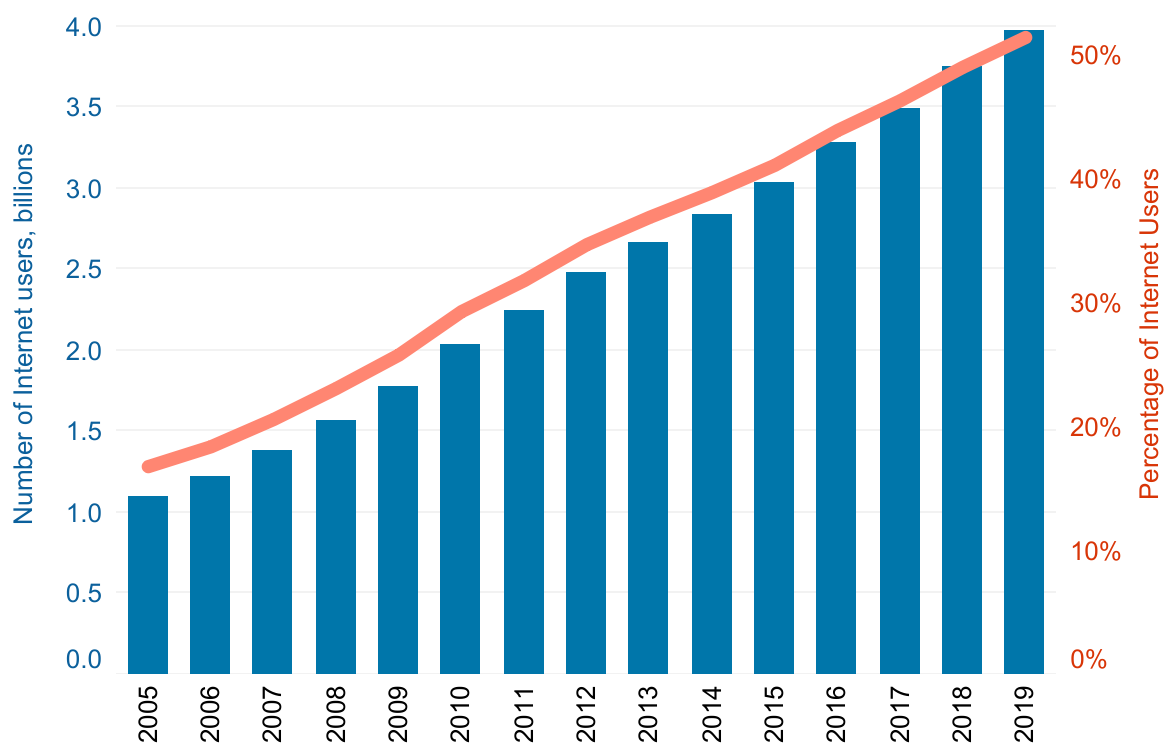
\includegraphics[width=.69 \textwidth]{./images/individuals_internet_2005-2019.png}
    \centering
    \caption{Individuals using the Internet from 2005-2019 \cite{ITU2019statistics}.}
    \label{Internet_Usage}
\end{figure}

\begin{figure}[h]
    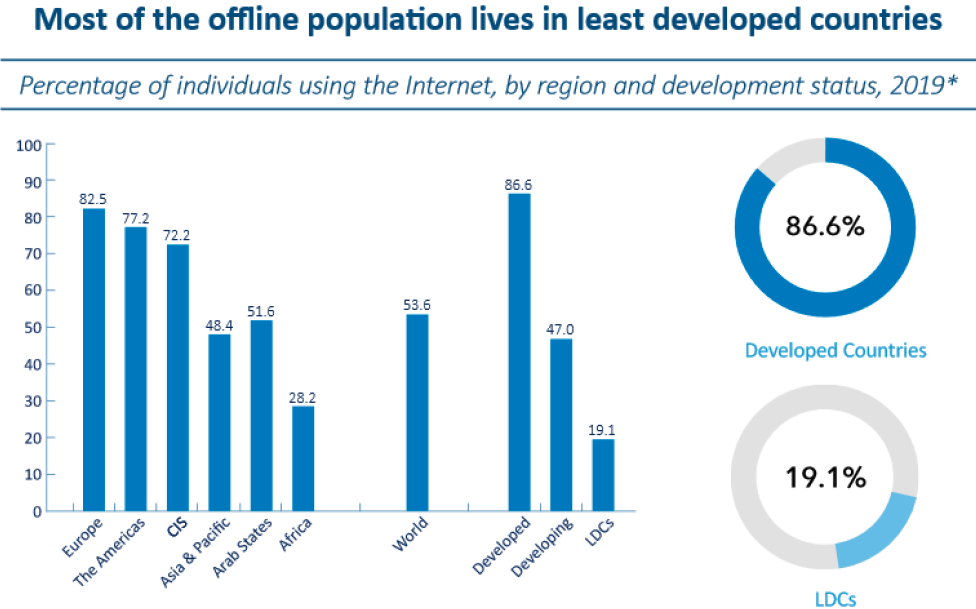
\includegraphics[width=.7 \textwidth]{./images/internet_usage_geography.png}
    \centering
    \caption{Percentage of individuals using the Internet by region and developmental status, 2019. The Commonwealth of Independent States (CIS) are the countries that were formerly part of the Union of Soviet Socialist Republics (USSR). The least developed countries (LDCs) are countries having the lowest indicators of socioeconomic development \cite{ITU2019statistics}.}
    \label{Internet_Usage_geography}
\end{figure}


%%%%%%%%%%%%%%%%%%%%%%%%%%%%%%%%%%%%%%%%%%%%%%%%%%%%%%%%%%%%%%%%%%%%%%%%
%%%%%%%%%%%%%%%%%%%%% Widespread Adoption of ICT %%%%%%%%%%%%%%%%%%%%%%%
\cleardoublepage
\subsection{Widespread Adoption of ICT Devices} \label{SECTION_WIDESPREAD_ADOPTION_OF_ICT}

In recent years there has been a proliferation of household electric and electronic equipment ownership. In 2019, approximately 1.57 million smartphones were sold globally \cite{statista2021phones} and its projected by 2022 that 2.13 billion units of personal computers, tablets and mobile phones will be shipped worldwide \cite{statista2021electronicsship}. Despite efficiency improvements in individual devices due to miniaturization (Figure \ref{ICT_embodied_emissions}), the net impact of the entire product community increased due to increased ownership, usage and faster turn-over of devices (Figure \ref{Household_ICT_Devices}) \cite{ryen2015consumption}. This has raised concerns regarding the emissions associated with these ICT devices (Sections \ref{SECTION_EMBODIED_EMISSIONS}-\ref{SECTION_END_OF_LIFE_EMISSIONS}), its unintended consequences (Section \ref{UNINTENDED_CONSEQUENCES}) and the unknown long term consequences of this rapid and widespread adoption.

\begin{figure}[h]
    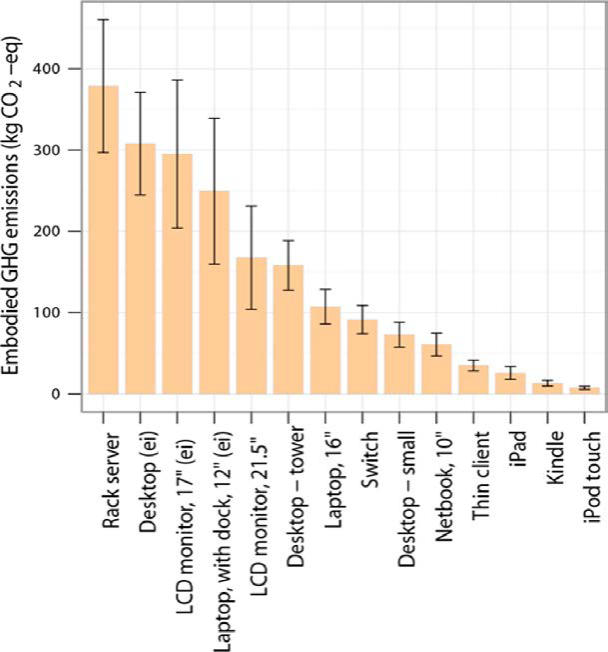
\includegraphics[width=.6 \textwidth]{./images/ICT_embodied_emissions.png}
    \centering
    \caption{Mean embodied GHG emissions with error bars showing $\pm$ two standard deviations. Due to miniaturization, embodied emissions of individual devices have been declining over time \cite{teehan2013comparing}.} 
    \label{ICT_embodied_emissions}
\end{figure}

\begin{figure}[h]
    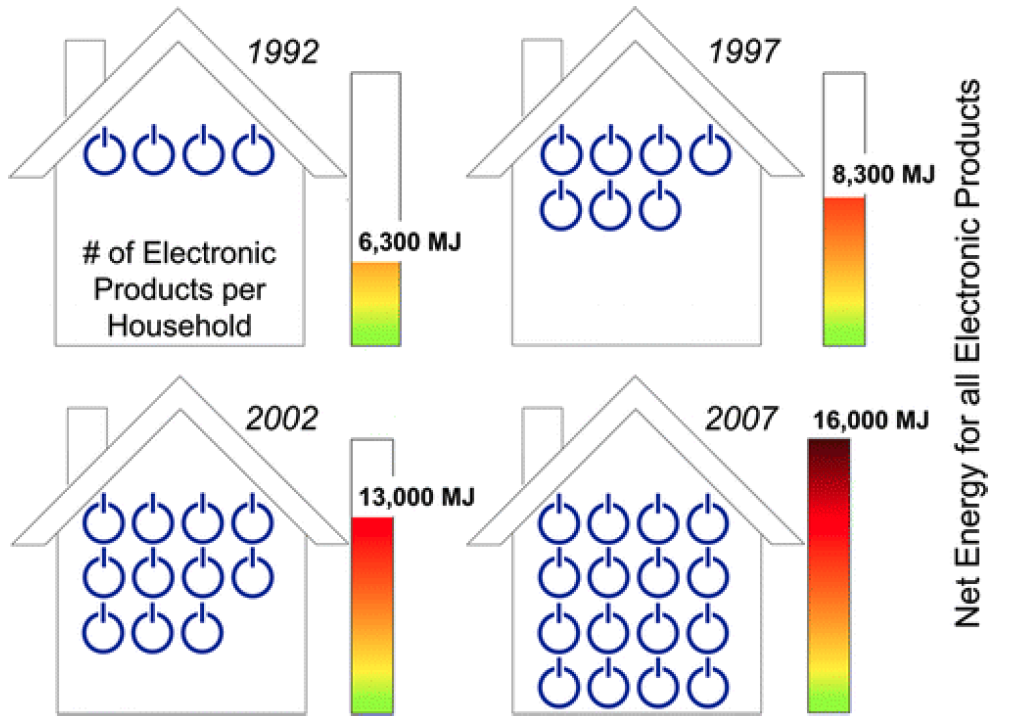
\includegraphics[width=.6 \textwidth]{./images/household_ICT_devices.png}
    \centering
    \caption{Consumption-weighted life cycle assessment methodology (LCA) for consumer electronics owned by an average U.S. household over a 15-year period (1992-2007) \cite{ryen2015consumption}.}
    \label{Household_ICT_Devices}
\end{figure}

% \begin{figure}[h]
%     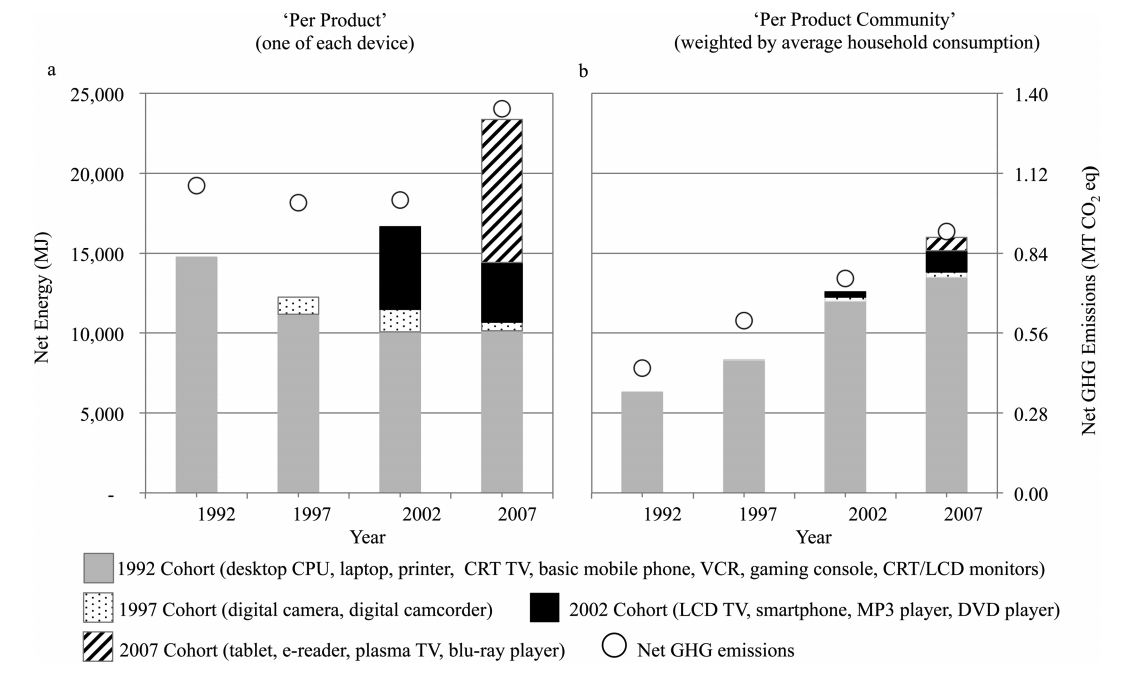
\includegraphics[width=.8 \textwidth]{./images/household_ICT_devices2.png}
%     \centering
%     \caption{\textit{Net annualized energy and GHG emission of electronics owned by U.S. households in 1992, 1997, 2002 and 2007. Data are aggregated by cohorts corresponding to the period in which groups of devices were introduced into the product community (indicated by color coding), and compared on a “per product” (ownership of one device per year) (a) and “per product community” basis (weighted by average household consumption trends) (b)} \cite{ryen2015consumption}.}
%     \label{Household_ICT_Devices2}
% \end{figure}

The major factors enabling this increased consumption of ICT devices globally are higher levels of disposable income, growing urbanization and mobility, and further industrialization \cite{forti2020global}. Contrary to popular belief, population growth is less of a driving force than affluence. A simple way to visualize this is the IPAT identity (Figure \ref{human_impact_PAT}), where the human impact (I) is an aggregate of changes in population (P), affluence (A) and technology (T).

\begin{figure}[h]
    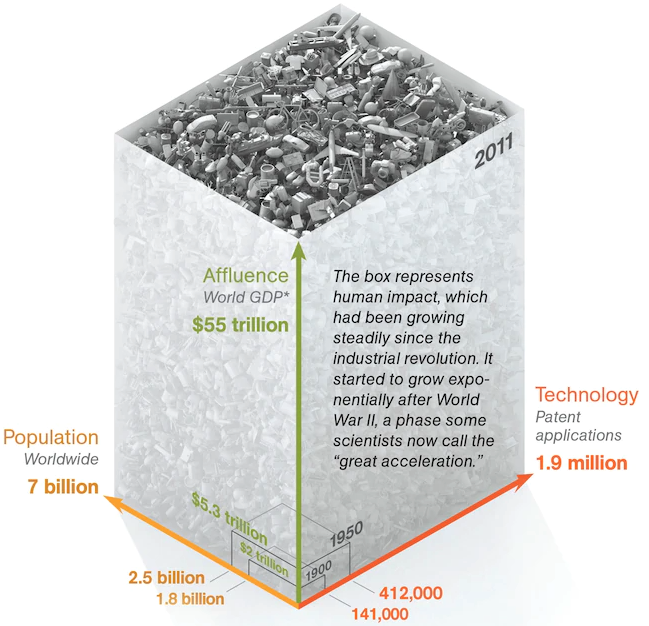
\includegraphics[width=.6 \textwidth]{./images/I=PAT_crop.png}
    \centering
    \caption{A depiction of the $I = P \times A \times T$ formula, where the volume represents the overall human impact (I) and the three axes represent the three drivers of population (P), affluence (A) and technology (T). Population is based on the number of people, affluence is based on the consumption per person and technology is based on the emissions per consumption. Note the difference in volume between the 1900–1950 period and the 1950–2011 period, which represents the Great Acceleration \cite{steffen2011anthropocene, nationalgeographic2014IPAT}.}
    \label{human_impact_PAT}
\end{figure}

%%%%%%%%%%%%%%%%%%%%%%%%%%%%%%%%%%%%%%%%%%%%%%%%%%%%%%%%%%%%%%%%%%%%%%%%
%%%%%%%%%%%%%%%%%%%%%%% Life Cycle Analysis %%%%%%%%%%%%%%%%%%%%%%%%%%%%
\cleardoublepage
\subsection{Life Cycle Assessment}
The ecological footprint of humanity is the demand that populations and activities place on the biosphere in a given year, based on the prevailing technology and resource management of that year \cite{borucke2013accounting}. This is calculated with respect to our carbon footprint, build-up land, forest, cropland, pasture and fisheries \cite{ecologicalfootprint2021}. Earth Overshoot Day marks the date when humanity's demand for ecological services in a given year exceed the Earth's capacity to regenerate it within that year. This deficit is realized by liquidating stocks of ecological resources and generating waste, which is primarily done by emitting carbon dioxide into the atmosphere. In 2020, humanity consumed their share of resources and achieved Earth Overshoot Day on August 22, 2020. The ecological footprint of humanity, however, is not evenly distributed across the globe. To encapsulate this, the date at which Earth Overshoot Day would fall if all of humanity lived like a specific country is also calculated (Figure \ref{Country_Overshoot_Days}). For example, if everyone were to live like Canada, the date would be moved up to March 18, 2020; in contrast, if everybody had the ecological footprint of Indonesia, we would almost make it to the end of year and Earth Overshoot Day would land on December 18, 2020 \cite{earthovershoot2020}.

 \begin{figure}[h]
    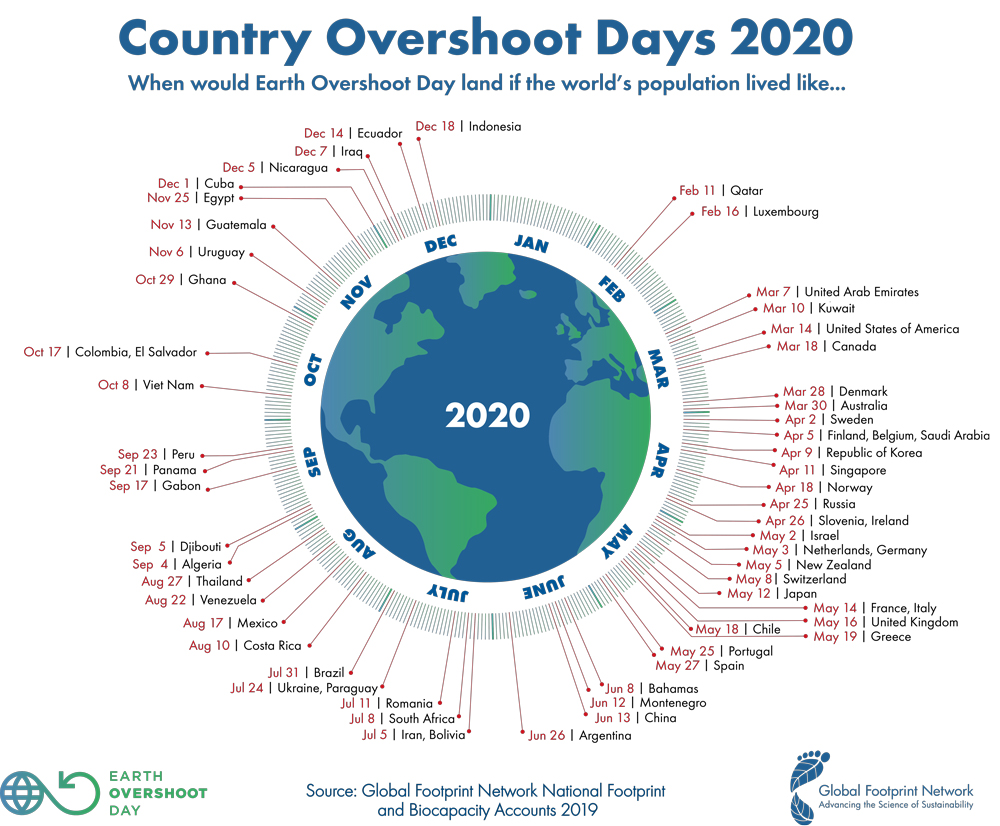
\includegraphics[width=.97 \textwidth]{./images/country_overshoot_days_2020.jpg}
    \centering
    \caption{Country overshoot days is the date on which Earth Overshoot Day would fall if all of humanity consumed like the people in this country \cite{earthovershoot2020}.}
    \label{Country_Overshoot_Days}
\end{figure}

As humanity continues to consume more than can be regenerated, the need for a methodology to properly encapsulate the full demand that ICT devices exact on our biosphere becomes apparent. The Life Cycle assessment is a systematic analytical method and model used to assess the potential environmental impacts and resources used through a product's entire life cycle from cradle to grave (Figure \ref{LCA_Stages}). The five stages in a product's life cycle are  \cite{finnveden2009recent, guinee2000life, andrae2015life}:
\begin{itemize}
    \item \textbf{Raw Material Acquisition:} the energy required to extract raw materials and the by-products produced
    \item \textbf{Manufacturing:} material processing and the production of %electricity, 
    intermediates, parts and the final product
    \item \textbf{Distribution:} the transportation and distribution of the product to consumers
    \item \textbf{Use Phase:} the use, reuse and maintenance of the product
    \item \textbf{End of Life:} storage, material recycling and waste management (incineration and landfill)
\end{itemize}

\begin{figure}[h]
    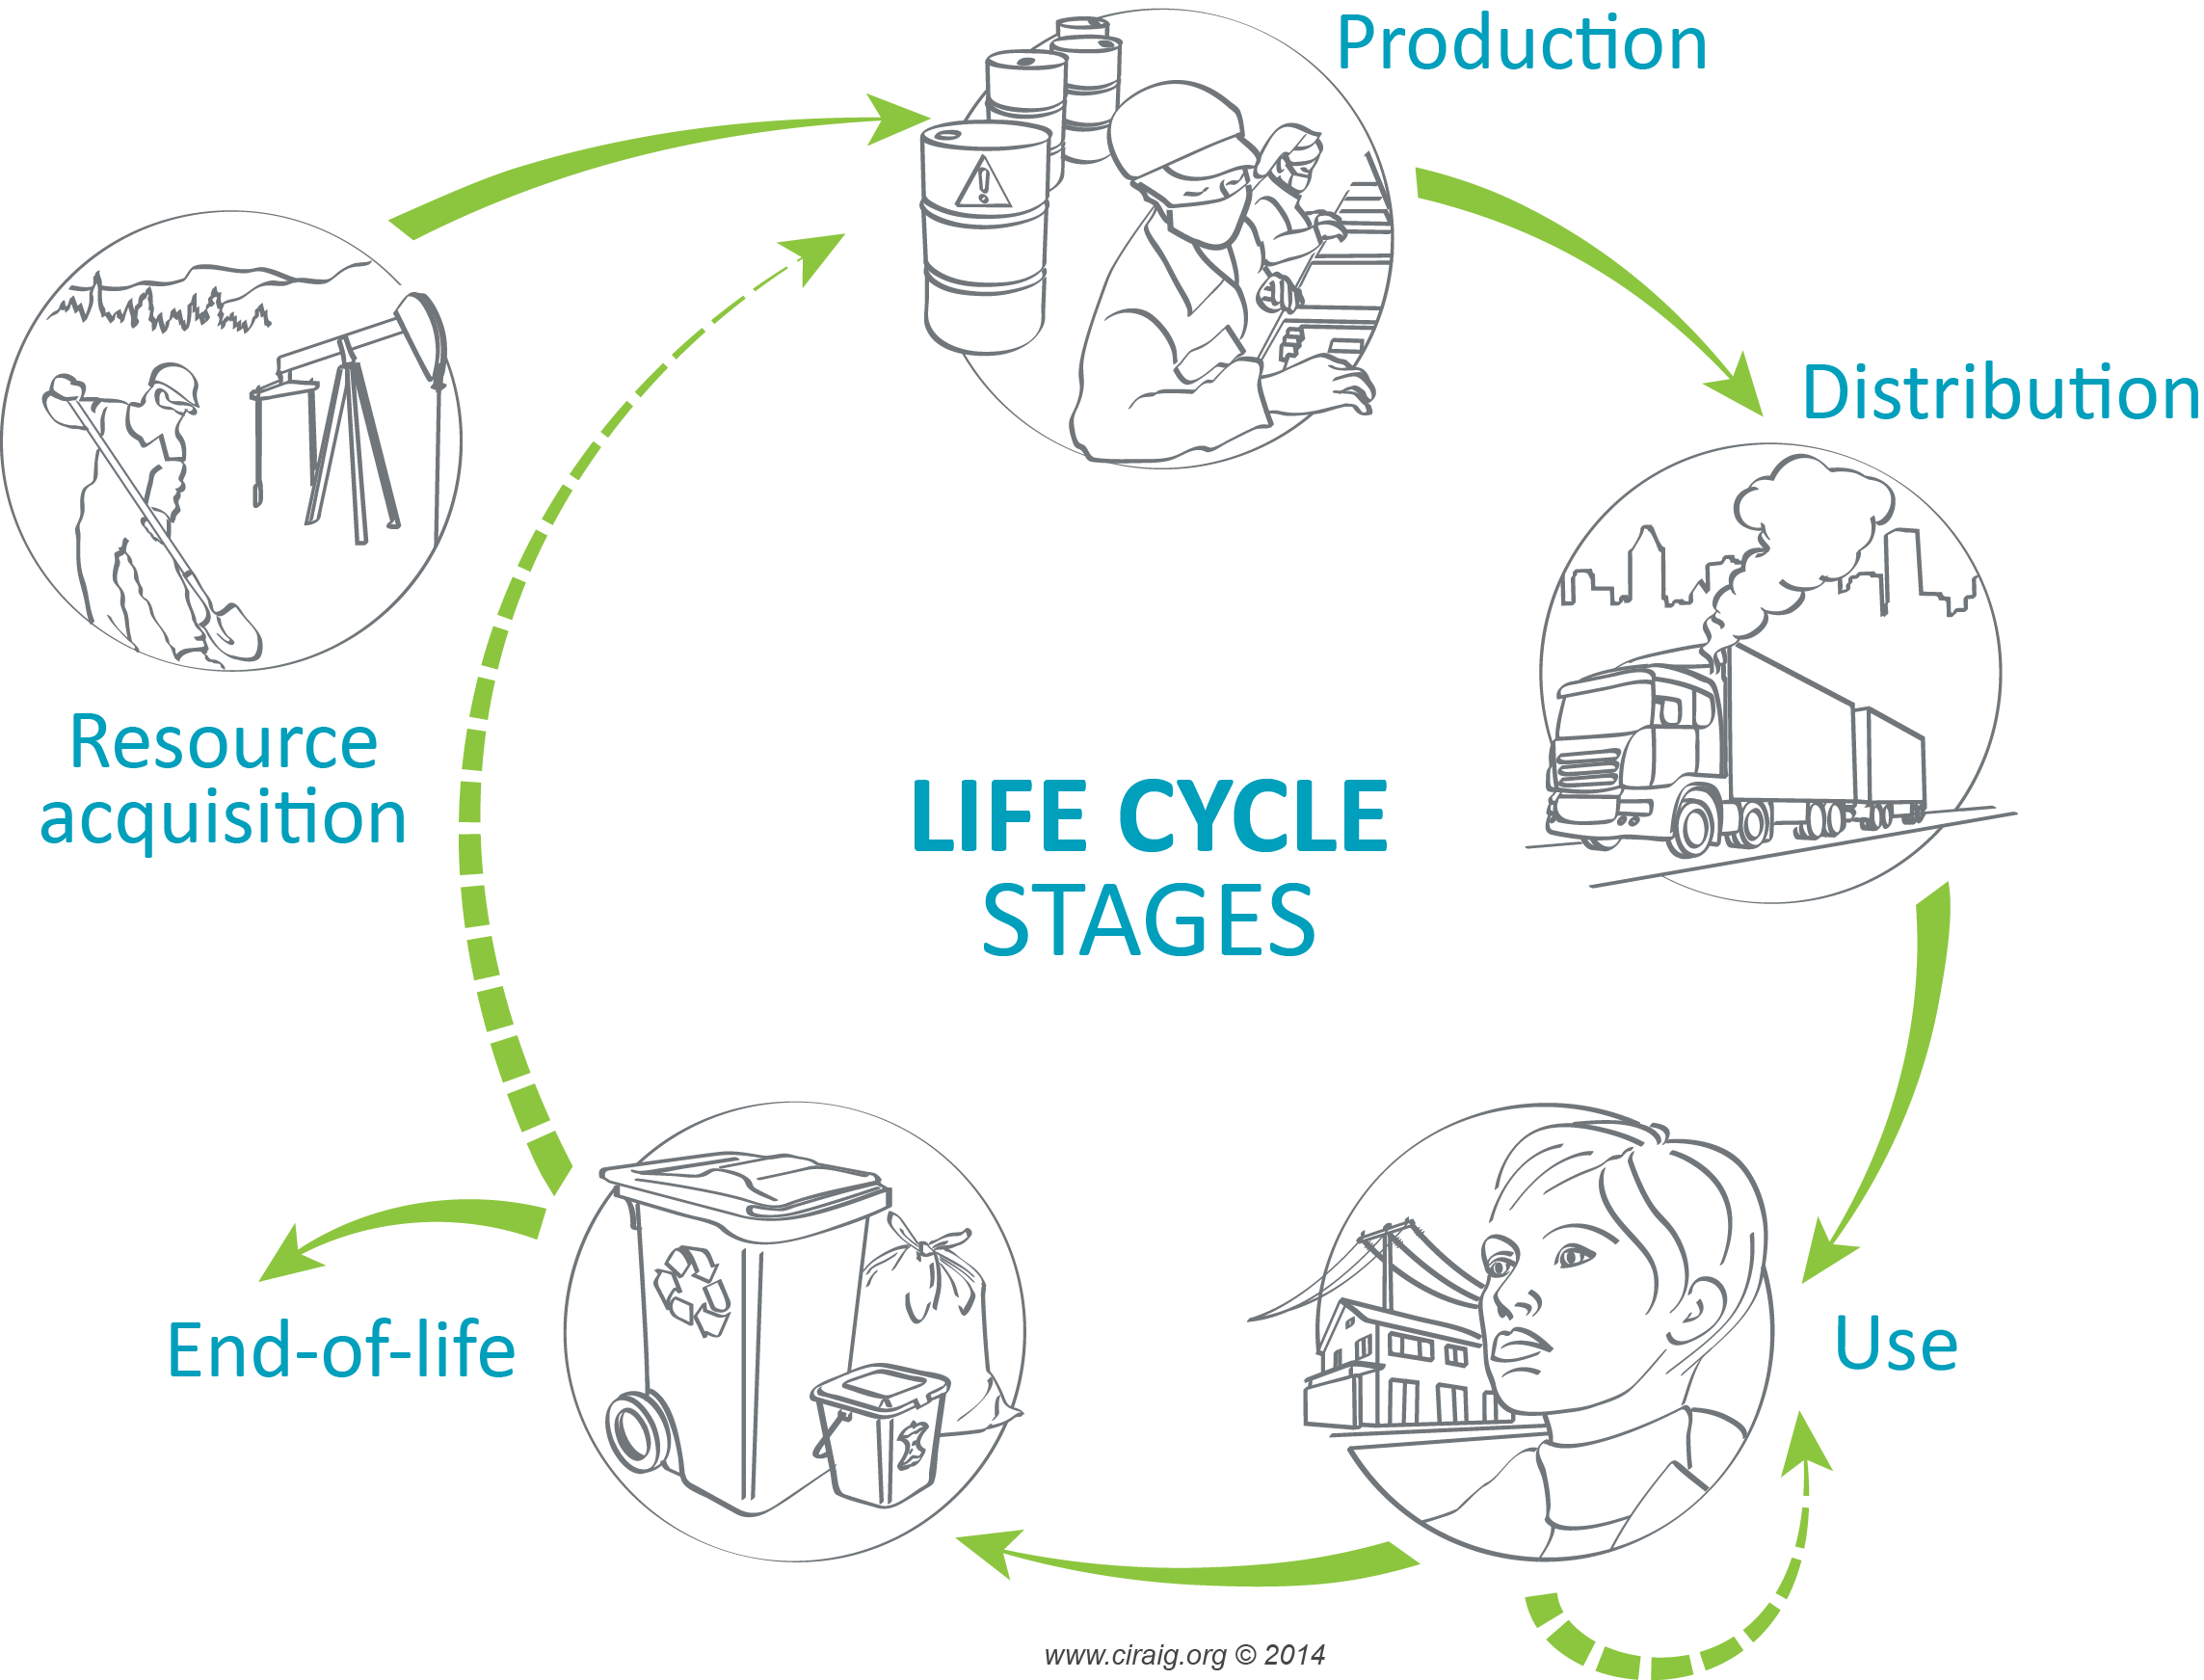
\includegraphics[width=.8 \textwidth]{./images/LCA_Stages1.png}
    \centering
    \caption{\textit{Stages of the life cycle assessment (LCA), a method to assess environmental impacts associated with all stages of a product's life from cradle to grave} \cite{ciraig2020LCA}}.
    \label{LCA_Stages}
\end{figure}

We will be using the life cycle assessment of ICT devices as the organizational framework of our paper; we will be examining each step in detail within the subsequent sections. Before we do so, however, we thought it important to mention that large electric appliances (washing machines, dryer, refrigerators, and freezers) have traditionally been responsible for the majority of household emissions, but now computers, televisions, and other ICT equipment are of comparable importance with respect to life cycle greenhouse gas (GHG) emissions (Figure \ref{ICT_devices_LCA}). As well, electronic devices tend to have a much higher production versus usage emissions. This is due to the costly extraction and processing of their component materials, as well as ICT devices being replaced or down-cycled far more frequently than their technical lifespan \cite{hertwich2011greenhouse}.

\begin{figure}[h]
    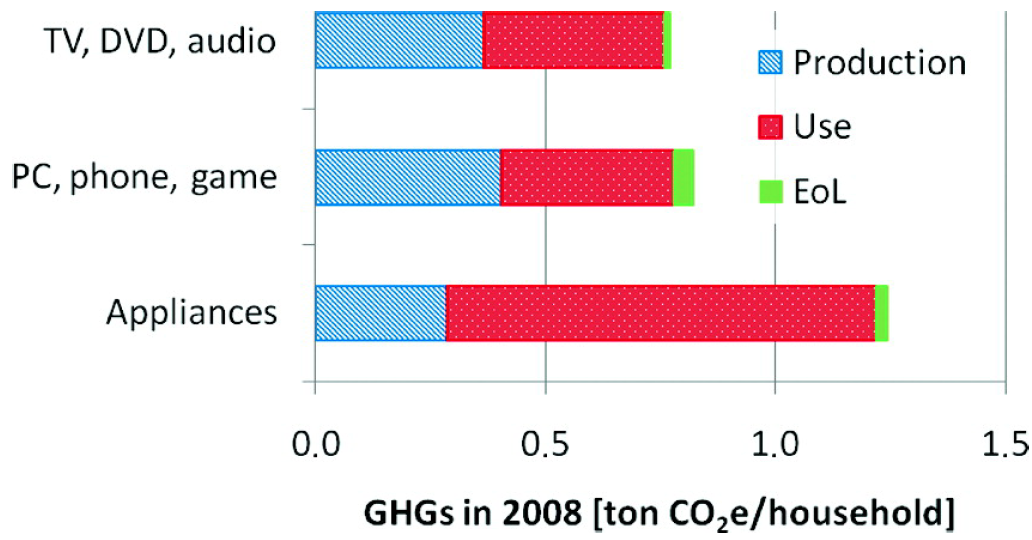
\includegraphics[width=.8 \textwidth]{./images/ICT_devices_LCA.png}
    \centering
    \caption{Life cycle greenhouse gas emissions for household electric and electronic equipment \cite{hertwich2011greenhouse}.}
    \label{ICT_devices_LCA}
\end{figure}

%%%%%%%%%%%%%%%%%%%%%%%%%% More LCA Readings %%%%%%%%%%%%%%%%%%%%%%%%%%%
\subsubsection{Further Readings for the LCA}
Although the LCA has been standardized for all types of products by the the International Organization for Standardization and for electronics by the European Telecommunications Standards Institute (ETSI) \cite{andrae2015life}, there is still variability and inconsistency between comparable ICT devices \cite{andrae2010life}. Often there is not much transparency in the emissions associated with the products that we buy. To address this, \cite{teehan2013comparing} presents a methodology to estimate the embodied emissions by using linear regressions based on product characteristics. For a LCA of specific ICT devices, see \cite{sikdar2013study} for wired and wireless local area network access, \cite{donovan2009twenty} for underwater fiber optic cables, \cite{andrae2017life} for virtual reality devices, and \cite{louis2020sources} for smartphones and tablet computers. For a review of LCAs for ICT products and services, please see \cite{arushanyan2014lessons}. A more rich discussion of the LCA methodology is in \cite{andrae2015life} and an in-depth analysis of the varying LCA methods is also summarized in Table 3 of the paper.


%%%%%%%%%%%%%%%%%%%%%%%%%%%%%%%%%%%%%%%%%%%%%%%%%%%%%%%%%%%%%%%%%%%%%%%%
%%%%%%%%%%%%%%%%%%%%%%%% Embodied Emissions %%%%%%%%%%%%%%%%%%%%%%%%%%%%
%%%%%%%%%%%%%%%%%%%%%%%%%%%%%%%%%%%%%%%%%%%%%%%%%%%%%%%%%%%%%%%%%%%%%%%%
\cleardoublepage
\section{Embodied Emissions} \label{SECTION_EMBODIED_EMISSIONS}
Embodied emissions refer to the emissions that occur in the ``upstream" life cycle stage, which correspond to the first two stages of the LCA resource extraction (Section \ref{SECTION_ACQUISITION_RAW_MATERIALS}) and production (Section \ref{SECTION_PRODUCTION}) \cite{teehan2013comparing}. 

%%%%%%%%%%%%%%%%%%%%%%%%%%%%%%%%%%%%%%%%%%%%%%%%%%%%%%%%%%%%%%%%%%%%%%%%
%%%%%%%%%%%%%%%%%% Acquisition of Raw Materials %%%%%%%%%%%%%%%%%%%%%%%%
\subsection{Acquisition of Raw Materials} \label{SECTION_ACQUISITION_RAW_MATERIALS}
Let us first examine the elements of a smartphone (Figure \ref{ELements_Of_Smartphone}). Although metals comprise approximately 30\% of its mass, less than 1\% of its weight is an assortment of ``spice metals": Tin (1\%), Silver (0.5\%), Gold ($<0.1\%$), Tantalum (trace), Palladium (trace), Indium (trace) and Rare Earth Elements (REE) \cite{bournay2006vital, compoundinterest2014, reller2009mobile}. For a more extensive breakdown of the raw materials and the manufactured parts of a smartphone, please see \cite{andrae2015life} (Table 1 and 2 respectively). 

\begin{figure}[h]
    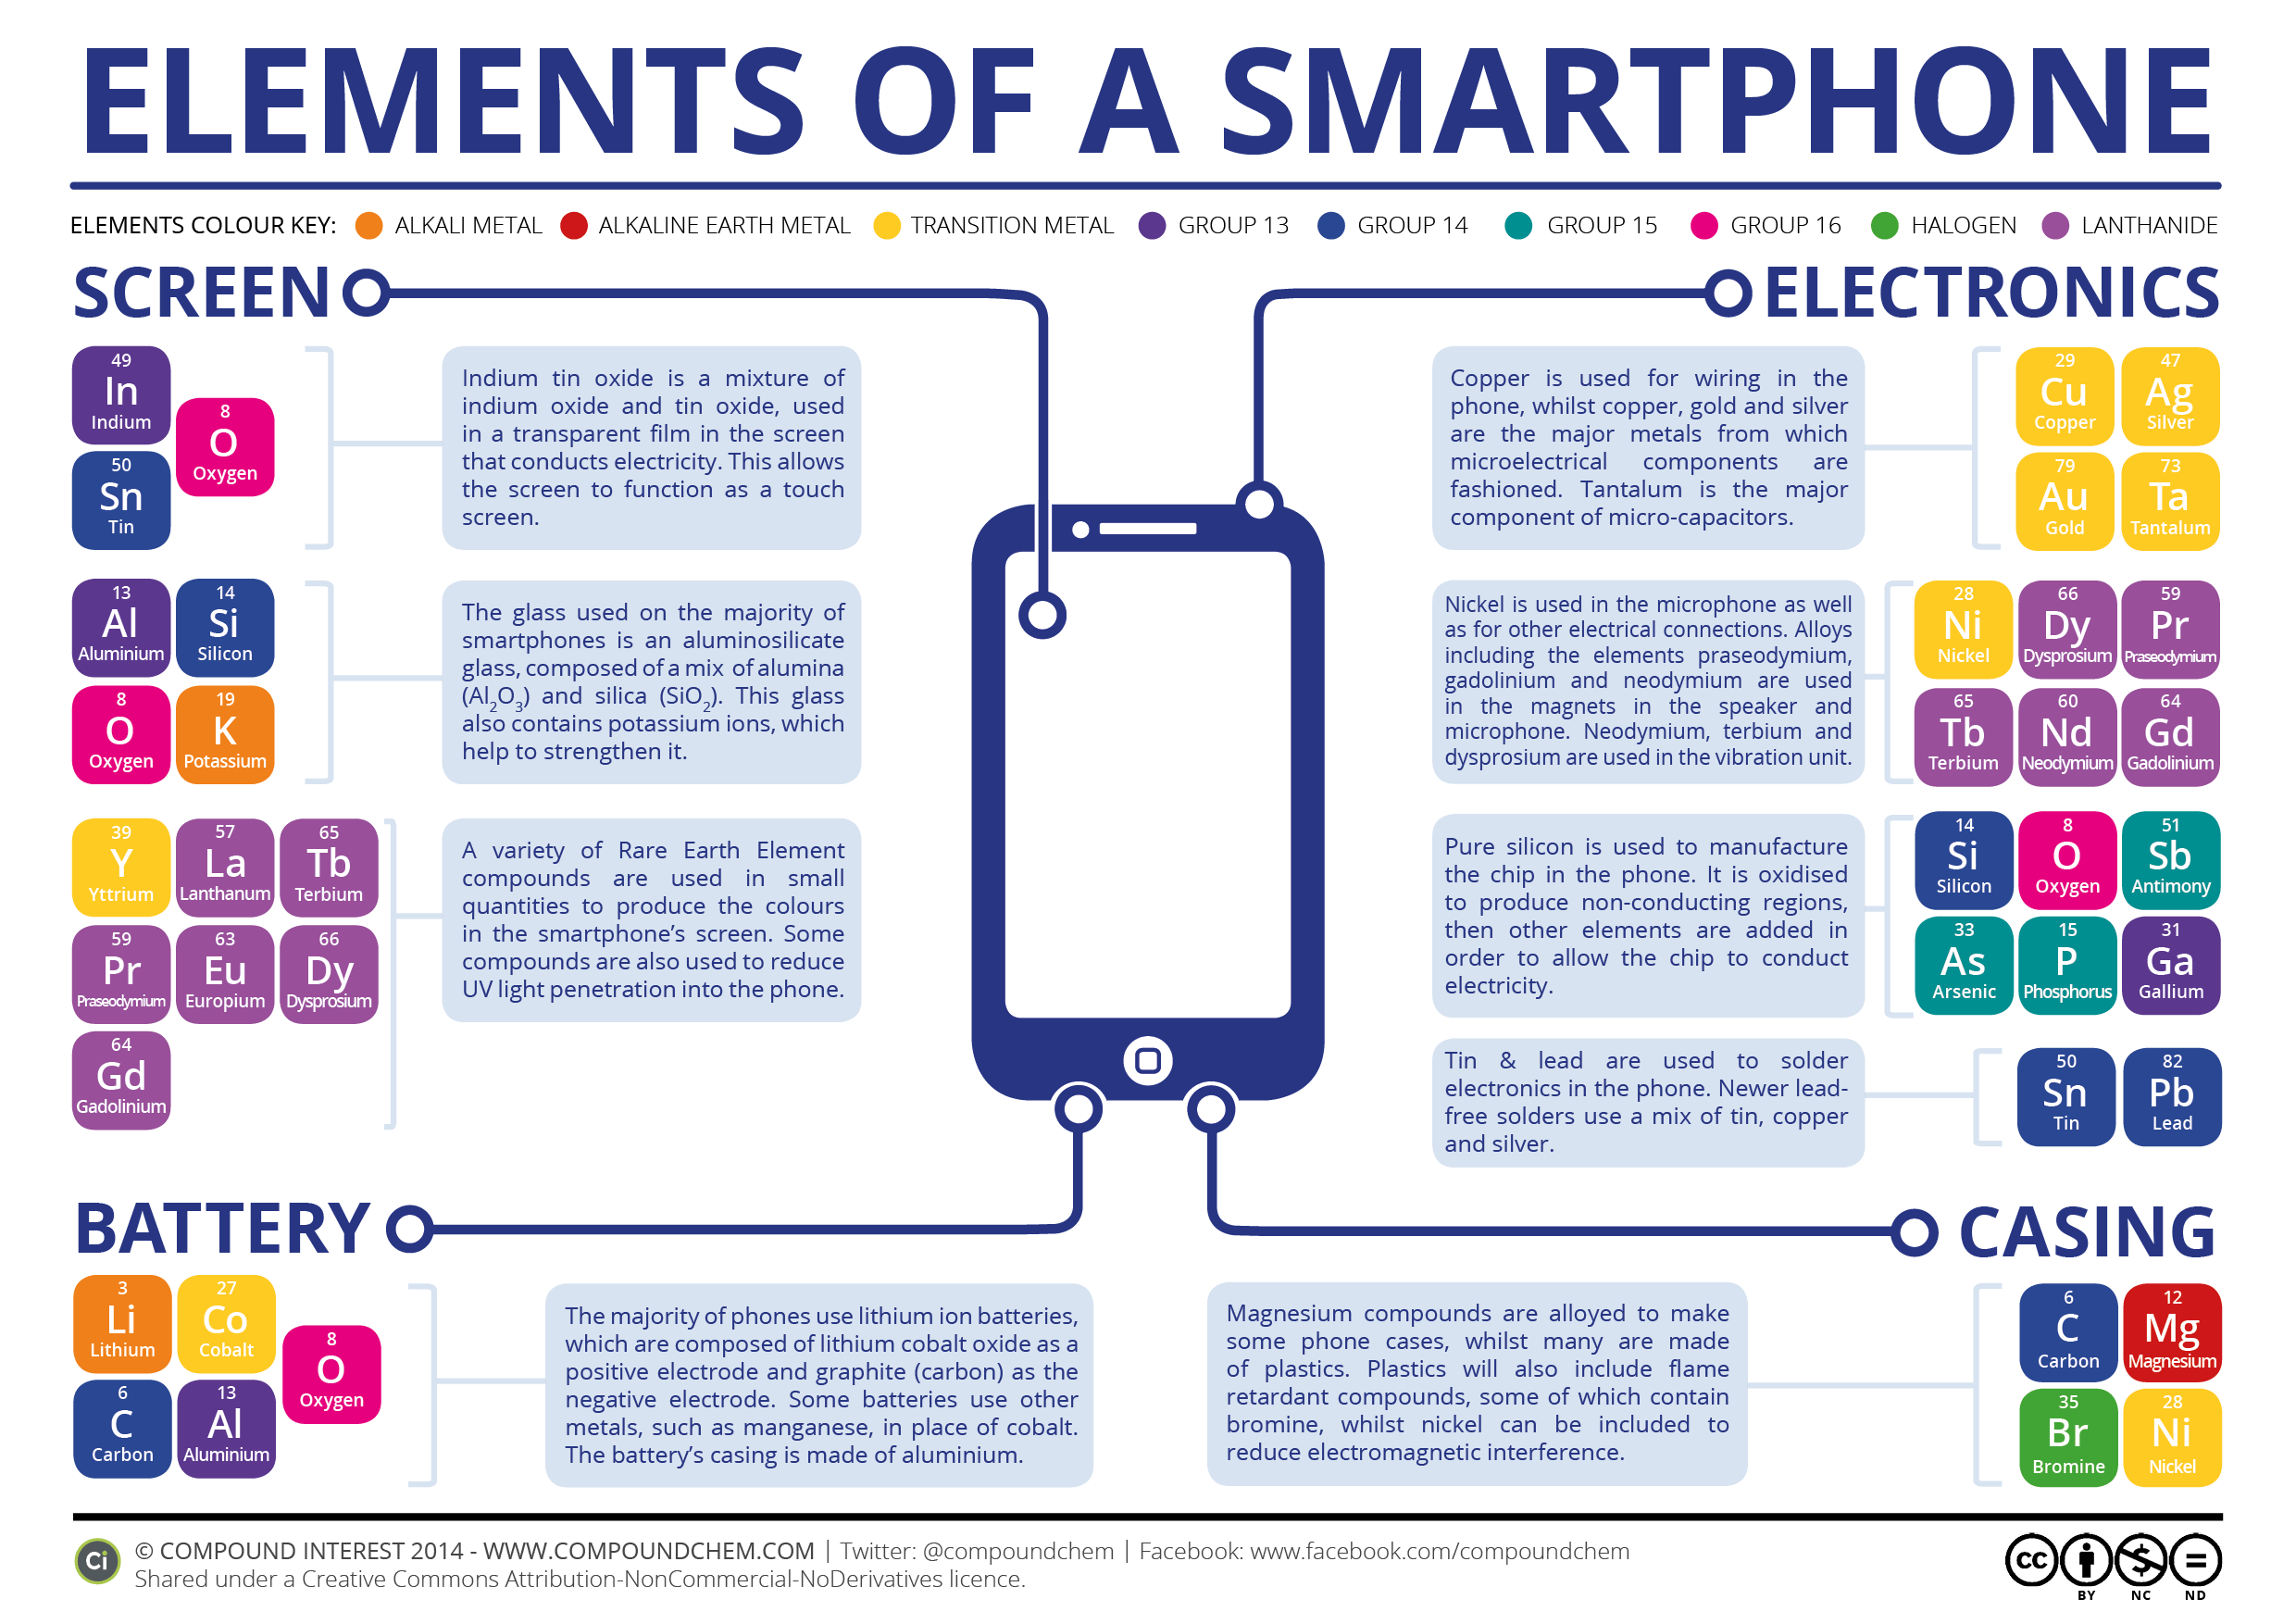
\includegraphics[width=.95 \textwidth]{./images/elements_of_smartphone.png}
    \centering
    \caption{Elements of a smartphone, broken down by its screen, electronics, battery and casing. The official name for Rare Earth Elements (REE) is Lanthanides (denoted by light purple colour) \cite{compoundinterest2014}.}
    \label{ELements_Of_Smartphone}
\end{figure}

A scarce mineral is one that occurs in low abundance or is geologically scarce. Often these are ``hitch-hikers", mined along with more abundant minerals. Examples of these scarce minerals and metals include cobalt (battery), indium (touch screen), tantalum (micro-capacitors) and rare earth elements (colours in screen, magents in speaker \& microphone, vibration unit) \cite{peiro2013material, compoundinterest2014}. In contrast, critical metals are not necessarily scarce; instead they have a high economic importance and a high risk associated with their supply. This supply risk is a combination of many factors, including substitutability, end-of-life recycling rates (see Section \ref{SECTION_END_OF_LIFE_EMISSIONS}), and a high geographical concentration of production in countries with poor governance \cite{eu2014criticalmaterials}.

The supply of rare earth metals ($>90\%$) are almost completely controlled by China \cite{schulz2018critical, physorg2012scarcemetals}, with 31\% just in the town of Bayan Obo. As well, China contains the vast majority of the world's reserves of indium which is essential to the production of screens \cite{reller2009mobile, eu2014criticalmaterials}. For the batteries, the majority of mobile devices use lithium batteries. Over 80\% of the world's lithium deposits are found in Chile, Argentina and Bolivia \cite{reller2009mobile}. Tantalum is the major component of micro-capacitors and four fifths of the world's supply is contained in Africa, of which 80\% is in the Democratic Republic of Congo (DRC) \cite{nzongola2002congo, montague2002stolen}. The DRC also supplies just over half of the world's supply of cobalt \cite{eu2014criticalmaterials}, a component essential for modern batteries.

Although substitutes may be found for these materials in the future, they are currently essential for the production of ICT devices and so the potential for geopolitical and economic disruptions to these reservoirs is non-trivial.


%%%%%%%%%%%%%%%%%%%% Environmental Impact %%%%%%%%%%%%%%%%%%%%%%%%%%%%%%
\subsubsection{Environmental Impact}
The five stages in the life of a mine are \cite{hartman2002introductory}
\begin{enumerate}
    \item \textbf{Prospecting}: searching for ores or other valuable minerals. This is typically performed by direct (physical geologic studies, aerial photography, satellite) and indirect (geophysics, geochemistry, geobotany) prospecting methods 
    \item \textbf{Exploration}: determining the extent and value of the mineral deposit. From here a feasibility study is created in order to determine whether to abandon or develop the mine.
    
    \item \textbf{Development}: opening a mineral deposit for exploitation. Preliminary development work typically consists of acquiring water and mineral rights, buying surface lands, arranging for financing, permit applications, and preparing an environmental impact statement (EIS). Construction of access roads, mineral transport systems, mineral processing facilities, waste disposal areas, offices, and other support facilities is then done. Depending on whether the minerals are to be mined at the surface or underground, the appropriate excavation method is performed. In surface mining, you must first strip the overburden, which is the waste material (soil, rocks, and living organisms) overlying the desired mineral product. Typical stripping ratios (ratio of waste rock removed to ore recovered) vary between materials and mining sites. For underground mining, these are generally much more complex and expensive; they consist of a carefully planned layout of access openings for mining. Surface mining is the dominant exploitation method worldwide. Almost all non-metalic minerals ($>95\%$), most metallic minerals ($>90\%$) and the majority of coal ($>60\%$) are mined by surface methods \cite{ramani2012surface}. 
    
    \item \textbf{Exploitation/Production}: the recovery of the minerals from the earth in quantity and the processing of them to separate the economically valuable minerals from their ores. For surface mining, aqueous methods and mechanical excavation methods including open pit, strip mining, and mountaintop-removal mining are typically employed \cite{lima2016legacy}; for underground mining, unsupported, supported and caving are used. In the ore processing phase, the valuable minerals are separated from the ore to yield a higher grade product (i.e. the higher the desired ore grade, the more waste produced). This results in a multitude of wastes, including contaminated mine water, tailings (a fine-grained mineral sand waste) and a variety of chemicals. With a few exceptions, the environmental impacts of metals are dominated by this purification and refining stage \cite{nuss2014life}.
    
    \item \textbf{Reclamation}: closure and restoration of the mining site. The best time to begin the reclamation process is before the first excavations are initiated so that the overall cost of mining plus reclamation is minimized (rather than just the cost of mining). One concern that needs to be addressed is the removal of office buildings, processing facilities, transportation equipment, utilities and other surface structures and the sealing of openings. The other chief concern is the restoration of the land surface, water quality and waste disposal areas. These goals tend to range from the avoidance of exposure to pollutants (remediation) to the full recovery of the original ecosystem (restoration). Unfortunately, restoration is typically unachievable, due to the mining site's altered hydrology, habitat fragmentation, contamination, climate change, and prohibitive costs \cite{lima2016legacy}.
\end{enumerate}

%Of the 30 billion tonnes of ore and waste materials mined each year, surface mining is responsible for 25 billion tonnes \cite{ramani2012surface}

One of the legacies of surfacing mining is the waste left behind. The extraction of 12 billion tonnes of ore is associated with the extraction of 19 billion tonnes of waste \cite{copco2007mining}. In the development stage, a large volume of waste rock needs to be excavated to reach the ore body (the amount of which depends on the stripping ratio). This waste rock is often stored nearby in piles or heaps. Since the composition of them varies, the elements of them leached into the environment also varies. Some elements are highly toxic even in small concentrations (for example, mercury), while others are less toxic but still pose a risk in higher concentrations (copper and zinc) \cite{geointro}.

In the exploitation stage, the tailings waste cannot be remediated and so they are stored in a slurry form and permanently contained behind a tailings dam to protect the surrounding environment. These tailings damns are some of the largest structures built by geotechnical engineers \cite{lyu2019comprehensive}. For reference, the Baotou tailings dam in Bayan Obo covers 11.5 km$^2$ and contains 150 million tonnes of tailings \cite{pan2016investigating}. In the reported 18,000 mines worldwide, the failure rate in the past one hundred years is approximately 1.2\%, which is two orders of magnitude greater than the 0.01\% failure rate of conventional water retention dams \cite{icold2001tailings}. A comprehensive review of over 300 tailing dam failures worldwide found that the major causes were seepage (21.6\%), foundation failure (17.3\%), overtopping (20.6\%), earthquake (17.0\%) and other (23.5\%). Although many accidents are related to natural events, such as heavy rain and earthquakes, each failure also involved engineering and human factors which could have been avoided \cite{lyu2019comprehensive}. When these failures occur they have a significant negative impact  on the ecosystems and human settlements downstream \cite{hudson2003impact}. Another issue that is more commonplace is the long-term leaching of contaminants of these tailings into surrounding water and land systems \cite{guo2013leaching}.

Using data back to the 1800s, we see an exponentially increasing trend for mining production, an exponentially increasing trend for waste rock and a gradual declining trend of ore grades. These ore grades are unlikely to ever increase in the future; in the case of gold, its ore grade is expected to decrease by half in the near future \cite{mudd2007sustainability}. An in-depth discussion of the LCA of specific metals is conducted in \cite{nuss2014life}. In their periodic table of global warming potentials (GWPs), the GWP per kilogram of each element\footnote{For reference, carbon dioxide has a GWP of 1} is 12,500 for gold, 3,880 for palladium, 260 for tantalum, 196 for silver, 102 for indium, 17.1 for tin and 12.6 for the REE tungsten.

%removal of the surface cover over the deposit, the changes to the original topography, the effects on soil and hydrologic conditions, the issues of mining and processing wastes, and the effect on the future economic potential of the mined areas and communities \cite{ramani2012surface}

%%%%%%%%%%%%%%%%%%%%%% Rare Earth Elements %%%%%%%%%%%%%%%%%%%%%%%%%%%%%
\subsubsection{Rare Earth Elements}
The global demand for rare earth elements---used in ICT devices, modern military equipment, and green technologies such as wind turbines, solar panels and hybrid vehicles---is continually increasing, resulting in a rapid growth of REE production and consumption. In addition to the challenges already mentioned, REE often ``hitch-hike" with radioactive elements (for example, thorium, uranium and radium) due to their similar chemical and physical attributes. The result is radioactive tailings and radioactive enrichment around REE mining and processing sites \cite{huang2016protecting} that may lead to growth inhibition, cytogenetic effects, and organ‐specific toxicity to abiotic and biotic systems \cite{pagano2015health, zhang2000chronic}.

There are over 1,000 identified REE deposits worldwide; however, only a few of them are being actively mined. In 2011, China produced approximately 95\% of REE materials, with the Bayan Obo mine in Northern China being the largest \cite{huang2016protecting}. Known as the ``death village", the surrounding village of Dalahai have experienced widespread intoxication of the farmland, animals and humans, including respiratory illnesses, cardiovascular disease, leukemia and cancer as a result of the mine \cite{huang2016protecting, eja2020bayanobo, dailymail2011bayanobo}. The potential geopolitical implications of this REE monopoly have been felt and is a source of concern \cite{gulley2018china, zhang2015did}, especially in the aftermath of China's sudden suspension of REE to Japan over a border dispute in 2010 \cite{ting2013rare} and now in 2021 as China explores limiting the export of REE to the United States of America (USA) that are crucial for their military \cite{financialtimes2021REE}.


%%%%%%%%%%%%%%%%%%%%%% Conflict Minerals %%%%%%%%%%%%%%%%%%%%%%%%%%%%%%%
\subsubsection{Conflict Minerals}
Conflict minerals are minerals that originate from the DRC or adjoining states and are processed into tin, tungsten, tantalum and gold (3TG) \cite{fitzpatrick2015conflict}, all of which are used in smartphones \cite{compoundinterest2014}. The Second Congo War (or Africa's First World War) was a devastating 6-year conflict involving at least six nations in the region. Characterized by extreme violence, mass population displacements, widespread rape and a collapse of public health services, the conflict resulted in the deaths of approximately 3.9 million people from 1998 to 2004 \cite{coghlan2006mortality}. %Despite being the largest humanitarian disaster in recent decades, there has been little response from the international community
Although the war has officially ended, it has since given way to a lower-intensity conflict in the eastern provinces of the DRC that continues to take a toll on the people living in the region \cite{coghlan2009update, cfr2021congoconflict}

Although a complex conflict with many narratives and underlying systematic structures outside the scope of this paper\footnote{As due diligence, we thought it imperative to mention the importance of not exclusively focusing on one cause of and one solution to the violence in the DRC. By focusing only on this single narrative, this has diverted attention from essential policy actions, the fight against corruption and the reform of the state administration; inadvertently this has exacerbated the very violence that proponents of this narrative were trying to reform \cite{autesserre2012dangerous}. Due to the scope of this paper, however, we will not be going into this further and we have instead given the reader an assortment of excellent resources that do.}
\cite{autesserre2012dangerous, alorse2015assessing, grant2015new}, one narrative we will focus on is the illegal exploitation of mineral resources that funds the conflict and perpetuates the violence (also referred to as the resource curse).

Four fifths of the world's supply of tantalum is contained in Africa, of which 80\% is in the DRC \cite{nzongola2002congo, montague2002stolen}. Despite 110 years of mineral extraction (untapped deposits are estimated to be worth \$24 trillion USD \cite{cfr2021congoconflict}), the wealth has not been used to better the citizens of the DRC; rather it has gone to the country's rulers and their political and business partners in the international community \cite{nzongola2002congo}. According to the United Nations' 2020 Human Development Index, the DRC ranks 175 out of 189, with 64\% of their population living in poverty \cite{unitednations2020hdr}.

For the trace mineral tantalum, ICT devices consumed approximately 15\% of global shipments and this total was estimated to increase to 27\% by 2018 \cite{fitzpatrick2015conflict}. For a more in-depth discussion of the tantalum supply chain, please see \cite{mancheri2018resilience}.


%%%%%%%%%%%%%%%%%%%%%% Conflicting Solutions %%%%%%%%%%%%%%%%%%%%%%%%%%%
\subsubsection{Conflicting Solutions}
Solutions to conflict minerals have been difficult due to the complex interactions at play. Policy solutions tend to aim for the goal of certifying minerals as conflict-free or initiatives for conflict-free sourcing. These include the Organisation of Economic Co-Operation and Development (OECD) Due Diligence Guidance \cite{oced2016duediligence}, the United Nations (UN) Guiding Principles on Business and Human Rights \cite{un2011guidingprinciples}, the European Union (EU) Conflict Minerals Regulation \cite{ec2020duediligence} and the industry led Conflict-Free Smelter Program (CFSP) \cite{cfsi2016cfsp}. As well, extractive taxes in Chile \cite{anrc2016chilecasestudy} and Norway \cite{lund2014state} have found success.

At a legislative level, the United States passed a provision of the Dodd-Frank Act act in 2010 to prevent the purchase of conflict minerals by compelling USA companies to audit their supply chains. Although well-intentioned, this unfortunately had unintended consequences. Due to the complex supply chains in the DRC \cite{moran2015global, reller2009mobile}, this has made it difficult for companies to determine if the supply is conflict free which has resulted in many multinational companies no longer buying from the DRC. This caused many miners to lose their jobs and their families to fall deeper into poverty, driving some to join the very armed militia groups the Dodd-Frank Act was attempting to target \cite{cfr2021congoconflict}. For DRC territories with an average number of gold mines, the passing of the Dodd-Frank Act increased the incidence of battles by 44\%, looting by 51\% and violence against civilians by 28\% \cite{stoop2018more}. 

From 2004 to 2014, there has been a 250\% increase in unaccounted production from small scale and artisanal mining \cite{mancheri2018resilience}. Officially, the DRC did not report any export of tantalum in 2013 or 2014. However, the import data from other countires shows 517 tons of tantalum was imported from the DRC. A discrepancy in Rwanda shows that 2,466 tons of tantalum were exported in 2013 but the country only produced 600 tons. This gap in official production numbers likely arises from rebel groups in the DRC smuggling tantalum across the border into Rwanda and Uganda where it is then exported \cite{mancheri2018resilience}.


%%%%%%%%%%%%%%%%%%%%%%%%%%%%%%% Cobalt %%%%%%%%%%%%%%%%%%%%%%%%%%%%%%%%%
\subsubsection{Cobalt}
Although not part of the 3TG minerals in the eastern DRC, the southern region of Katanga supplies 60\% of the world's cobalt---no other country produces more than 6\% \cite{shedd2017cobalt}---which is essential for lithium-ion rechargable batteries in your phone, computer, and electric vehicles. Due to the relative level of peace in Katanga compared to the eastern provinces of the DRC and the mines not being controlled by armed rebel groups, the mines here are not seen as ``conflict minerals". There is however widespread instability, violence and minimal rule of law surrounding the mines \cite{scheele2016cobalt}.

The formal industrial cobalt mines in the DRC are controlled by Congolose state-owned and foreign companies \cite{scheele2016cobalt}, with China having a major influence \cite{gulley2019china}. These companies have been associated with labour rights violations, community conflicts and land grabs \cite{scheele2016cobalt}. Studies have also found that people living within 3 km of industrial mines and smelters have high levels of exposure to cobalt and other trace elements \cite{banza2009high}. In the last three decades, there has been a growth of locals participating in the artisanal and small-scale mining (ASM) sector. Although the share of cobalt from ASM is difficult to determine due to its informal and often illegal nature, an estimated 15-20\% of cobalt in the DRC is extracted this way \cite{al2017cobalt}. Widespread child labour is employed here \cite{andre2014child} and despite the potentially fatal health effects of prolonged exposure to cobalt \cite{nkulu2018sustainability}, adult and child miners often work without basic protective equipment, including gloves, work clothes or masks.  Artisanal miners manually dig their own mines, often extending far underground without any supports and poor ventilation, resulting in the frequent collapse of unsupported tunnels \cite{al2017cobalt, amnesty2016drc}. Once extracted, the ores are sold to traders who then sell it to Chinese, Indian, or Lebanese companies who then export them to cobalt refining countries including China, Belium, Finland and Canada \cite{al2017cobalt}.


%%%%%%%%%%%%%%%%%%%%%%%%%%%%%%%%%%%%%%%%%%%%%%%%%%%%%%%%%%%%%%%%%%%%%%%%
%%%%%%%%%%%%%%%%%%%%%%%%%%%% Production %%%%%%%%%%%%%%%%%%%%%%%%%%%%%%%%
\cleardoublepage
\subsection{Production} \label{SECTION_PRODUCTION}
For an ICT device, you typically have the following basic components: a central processing unit (CPU), memory (for example, random access memory (RAM)), circuit board (including the motherboard), storage (hard disk, and solid-state drives (SSD)), network connection, battery, and input/output devices \cite{bourgeois2014information}.

For the CPU, you need a semiconductor microchip which consists of a highly purified silicone wafer (to be of Electronic Grade Silicon, you may only have 1 alien atom for every billion silicon atoms \cite{intel2011makingachip}). Although this high purity is integral to modern computing efficiency, the production of silicone wafers requires 160 times the energy required for typical industrial grade silicon \cite{williams20021}. Next comes the fabrication of chips on a silicon wafer that creates a series of patterned layers of various materials. This fabrication stage consists of hundreds of precisely controlled steps, including ion implantation, high-k dielectric deposition, photo lithography, etching, metal deposition, and metal layering. Finally, these wafers are tested, sliced into dies and then assembled with a heatspreader (a thermal interface that keeps the processor cool during operation) to form the completed processor \cite{intel2011makingachip}. A diagram of this process is summarized in Figure \ref{production_chip}. To produce a single 2-gram 32MB DRAM chip, the process requires approximately 1,600g of fossil fuels, 72g of chemical inputs and 32,000g (32L) of water. The fossil fuels used in production total 600 times the mass of the final product; in comparison, automobiles and refrigerators have a factor of  1-2 \cite{williams20021}. Although these new methods yield more precise small-scale devices, performing thermal oxidative processes to produce thin layers of oxidized silicone has resulted in a large increase in energy demand to produce semi-conductor chips  \cite{gutowski2009thermodynamic}.

\begin{figure}[h]
    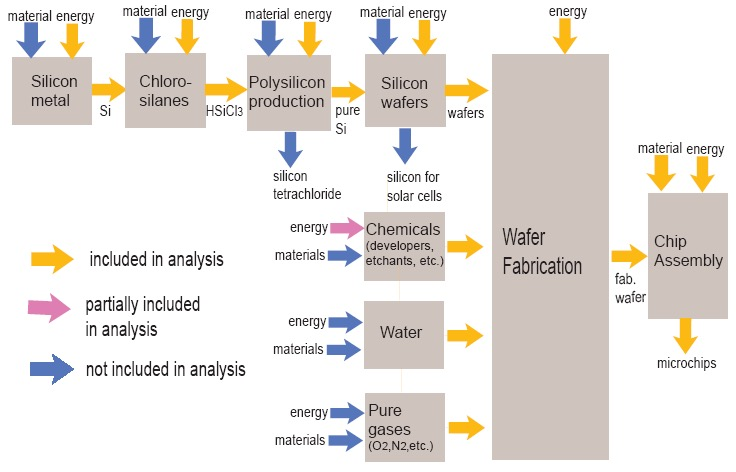
\includegraphics[width=.9 \textwidth]{./images/production_chip.jpg}
    \centering
    \caption{Network of manufacturing processes in chip manufacturing \cite{williams2004environmental}.}
    \label{production_chip}
\end{figure}

In general most greenhouse gas emissions come from the production stage, specifically during the manufacturing of the printed circuit board. As well, smaller devices, smaller screens, and devices with less memory tend to have less embodied greenhouse gas emissions \cite{louis2020sources, teehan2013comparing}. Overall embodied greenhouse gas emissions for newer products are 50-60\% lower than corresponding older products with similar functionality. This decrease can largely be attributed to a reduction in total mass and a proportional decrease in integrated circuit content \cite{teehan2013comparing}. Although we are producing more efficient devices, our demand for what they can do has also increased. Since the 1960s, our processing power has exponentially grown with a doubling time of almost 2 years, as observed by Moore's Law \cite{schaller1997moore}.


%%%%%%%%%%%%%%%%%%%%%%%%%%%%%%%%%%%%%%%%%%%%%%%%%%%%%%%%%%%%%%%%%%%%%%%%
%%%%%%%%%%%%%%%%%% Resonsibility of Emissions %%%%%%%%%%%%%%%%%%%%%%%%%%
\subsection{Responsibility of Emissions}\label{SECTION_RESPONSIBILITY_OF_EMISSIONS}
The international community takes a production-based approach to measuring a country's emissions: a country is responsible for the emissions associated with the extraction of raw materials, production of goods and disposal of waste within their borders. This system forms the basis of the United Nations Framework Convention on Climate Change (UNFCCC) international carbon accounting systems and efforts to mitigate carbon emissions, including the Kyoto Protocol and the Paris Agreement \cite{unfccc2009kyoto, unfccc2015paris}. This accounting decision means a country's emission reduction commitments do not include emissions attributed to their imports---essentially, countries are allowed to export their emissions. This has coincided with a shift of energy intensive industries from developed to developing countries, which often are less energy efficient. For example, 23\% of China's total CO$_2$ emissions in 2004 came from its net exports (Figure \ref{emissions_China_export}) \cite{wang2007owns}.

\begin{figure}[h]
    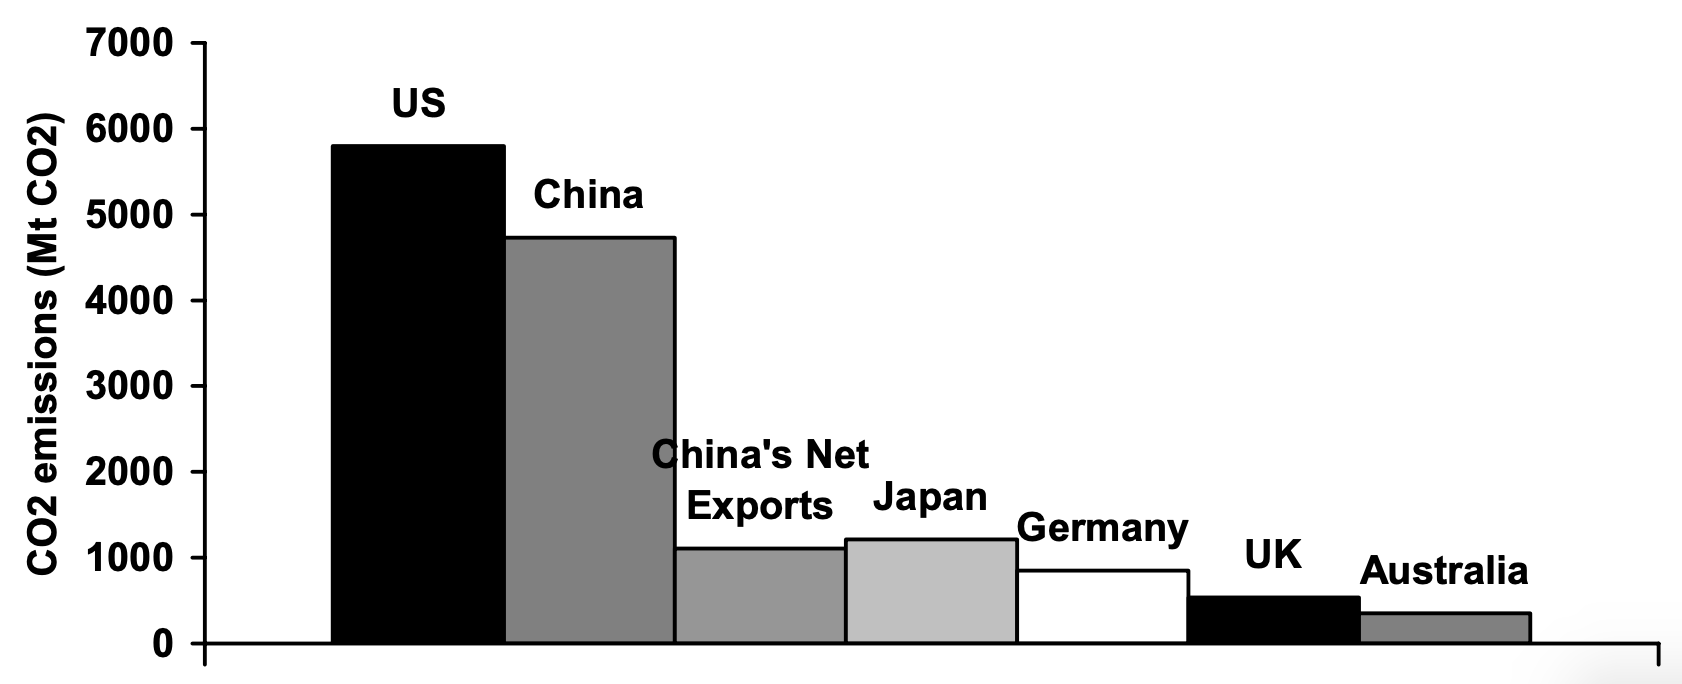
\includegraphics[width=.9 \textwidth]{./images/emissions_China_export.png}
    \centering
    \caption{CO$_2$ emissions from China's net exports in 2004 in comparison with selected national emissions figures \cite{wang2007owns}.}
    \label{emissions_China_export}
\end{figure}

By measuring emissions based on production, rather than consumption, it raises the issues of equity: who is responsible for the emissions? Should responsibility for
emissions be allocated to countries that \textit{produce} goods and services or to the countries that \textit{consume} the products and services? Critiques and potential improvements to this metric have been discussed \cite{tukker2020consumption, wang2007owns} and we recommend the reader to dive into them further if interested. Although international accounting methodologies is beyond the scope of the paper, the majority of ICT emissions come from its production emissions \cite{hertwich2011greenhouse} and so we thought it important to briefly mention.


%%%%%%%%%%%%%%%%%%%%%%%%%%%%%%%%%%%%%%%%%%%%%%%%%%%%%%%%%%%%%%%%%%%%%%%%
%%%%%%%%%%%%%%%%%%%%%%%%%%% Distribution %%%%%%%%%%%%%%%%%%%%%%%%%%%%%%%
%%%%%%%%%%%%%%%%%%%%%%%%%%%%%%%%%%%%%%%%%%%%%%%%%%%%%%%%%%%%%%%%%%%%%%%%
\cleardoublepage
\section{Distribution}
Once an ICT device is manufactured, it must be packaged and transported either to stores or directly to customers. Since there is not much in the distribution phase that is ICT specific, we will give a brief background and refer out to appropriate resources.

%%%%%%%%%%%%%%%%%%%%%%%%%%%%%%%%%%%%%%%%%%%%%%%%%%%%%%%%%%%%%%%%%%%%%%%%
%%%%%%%%%%%%%%%%%%%%%%%%%%% Packaging %%%%%%%%%%%%%%%%%%%%%%%%%%%%%%%%%%
\subsection{The Packaging Nightmare}
During a product's journey from manufacturer to customer, the product must be protected from dirt and shocks and contained. There is also an increasing demand for other packaging requirements, such as making the product easier to store and effectively displaying and promoting the product \cite{rundh2005multi}. To meet these demands, an entire field has emerged to design the most suitable packaging: cardboard boxes, glass jars, plastic bags, plastic film, plastic bottles, aluminum wrappers, and expanded polystyrene, to name a few. Packaging has a particularly short lifespan; it becomes waste as soon as its contents reach its destination. 
%One of the most prolific packaging is the plastic bag, of which approximately 500,000,000,000 are distributed a year worldwide. It has a very limited lifespan, however. It takes 1 second to manufacture, 20 minutes to use and approximately 100-400 years to degrade naturally.
While this limited lifespan has been a boon for the packaging sector, it has become a serious challenge for waste management \cite{bournay2006vital}. We will speak extensively in Section \ref{SECTION_END_OF_LIFE_EMISSIONS} about the challenges of the e-waste generated from ICT, but it is worth mentioning that packaging waste constitutes a large proportion of household waste. In the case of some countries it is the majority (Figure \ref{packaging_waste}). 

\begin{figure}[h]
    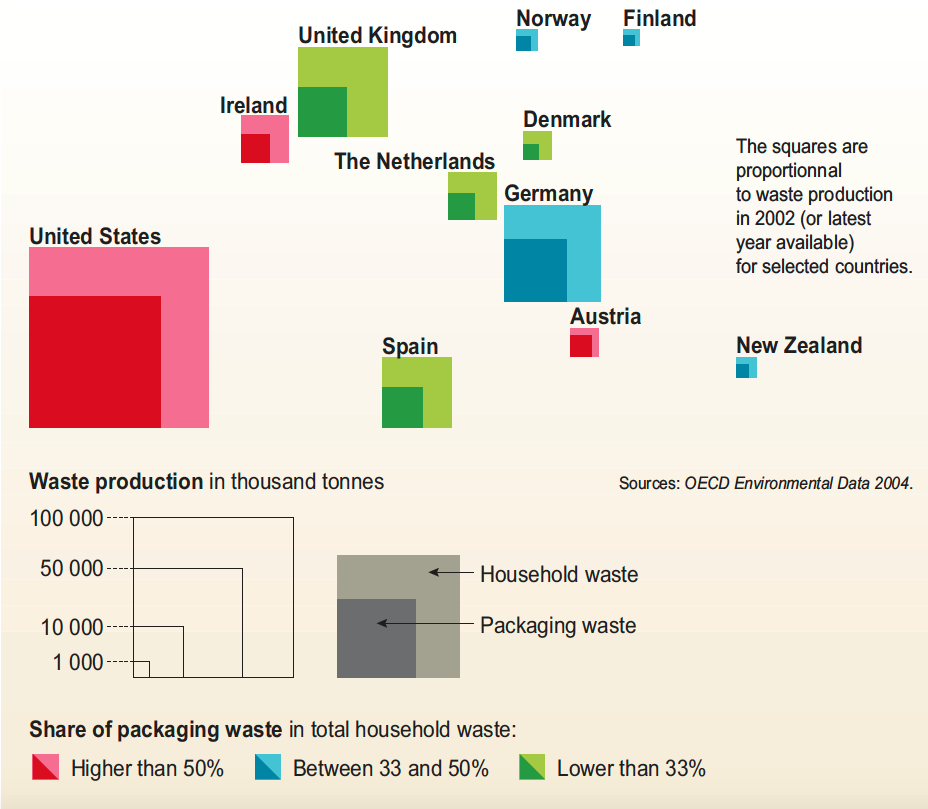
\includegraphics[width=.85 \textwidth]{./images/packaging_waste.png}
    \centering
    \caption{The amount of household waste produced for selected countries in 2002. The proportion of waste that comes from packaging is also depicted \cite{bournay2006vital}.}
    \label{packaging_waste}
\end{figure}

In addition to the large quantity of packaging waste, the recycling rates of different packaging materials vary from 20\% for plastics to 70\% for paper \cite{bournay2006vital}. Although there has been some movement towards more environmentally friendly packaging \cite{min1997green, cinelli2019cosmetic, chiellini2008environmentally, moustafa2019eco}, the literature is quite sparse. Having more recyclable packaging is important but it does not address the systematic problem of overpackaging, lack of reusability and sales packaging. For a good overview of the challenges faced and a LCA on packaging, please see \cite{lee2005design}.


%%%%%%%%%%%%%%%%%%%%%%%%%%%%%%%%%%%%%%%%%%%%%%%%%%%%%%%%%%%%%%%%%%%%%%%%
%%%%%%%%%%%%%%%%%%%%%%% Transportation %%%%%%%%%%%%%%%%%%%%%%%%%%%%%%%%%
\subsection{Transportation}
Despite most of the design phases remaining in the United States, since the 1990s the actual production of computers and its components has shifted from the United States to the Asia-Pacific region \cite{kraemer1998globalization}. This has resulted in the largest interrgional export of embodied emissions from computers originating from China and being shipped to the United States, the European Union and Japan (Figure \ref{transport_global_computers}). Although there are economic incentives for this, the emissions associated with this global transportation are substantial. 
Statistics on the emission associated with shipping just ICT products could not be found; however, the fuel consumption for the 2001 internationally registered fleets (cargo vessels, other commercial vessels and military vessels) was estimated to be 289 million tonnes (289,000,000,000 kg) \cite{corbett2003updated}.

\begin{figure}[h]
    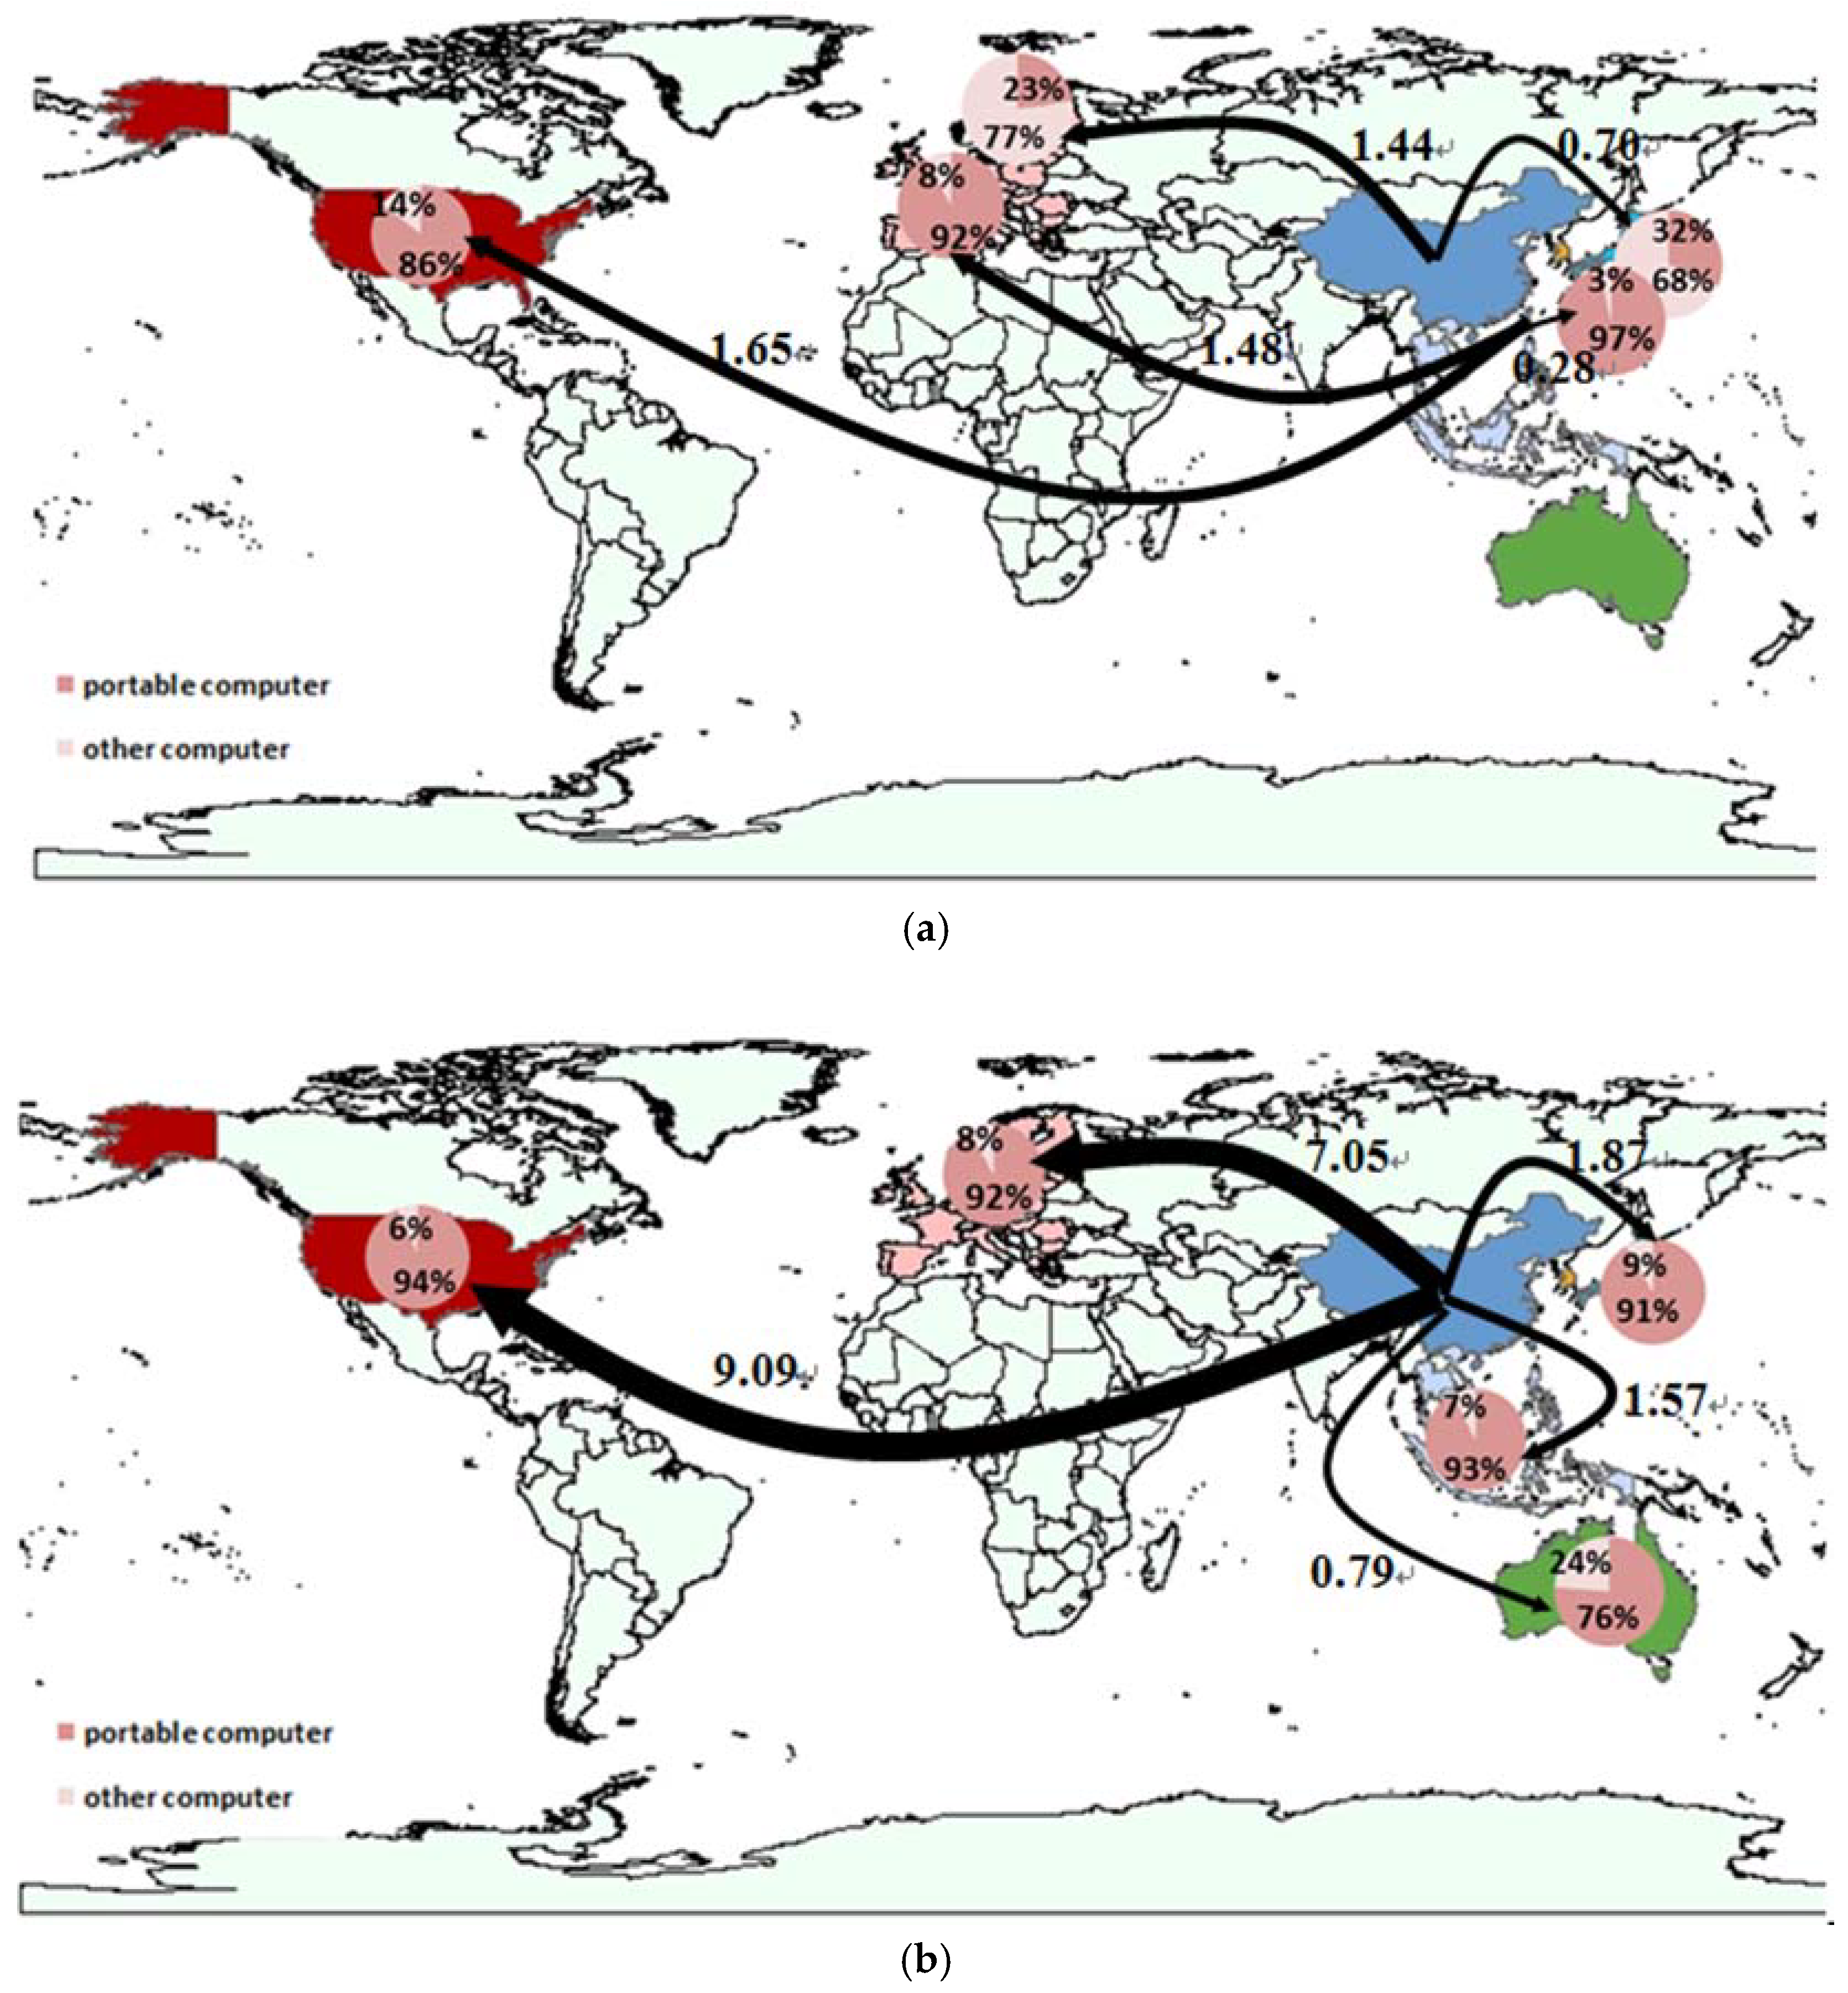
\includegraphics[width=.85 \textwidth]{./images/transport_global_computers.png}
    \centering
    \caption{\textit{Top 5 largest interregional flows of emissions (Mt of CO$_2$-eq) embodied in trade of computers (aggregated to portable computers and other computers) in 2002 (\textbf{a}) and 2013 (\textbf{b})} \cite{lee2018greenhouse}.}
    \label{transport_global_computers}
\end{figure}

From here a good needs to arrive in a consumer's hand either by a trip to a traditional brick-and-mortar store or by online shopping. There are many factors at play here which vary greatly across global demographics, geography, behaviours, transportation method used, and the speed of deliveries. Since this is not ICT specific we will not be doing an in-depth discussion. If you are interesting in this aspect of the LCA, \cite{carling2015measuring, jaller2020evaluating, brown2014carbon} provide a fruitful discussion of the nuances, challenges and limitations of evaluating online and in-store shopping.


%%%%%%%%%%%%%%%%%%%%%%%%%%%%%%%%%%%%%%%%%%%%%%%%%%%%%%%%%%%%%%%%%%%%%%%%
%%%%%%%%%%%%%%%%%%%%%%%%%%% Usage Emissions %%%%%%%%%%%%%%%%%%%%%%%%%%%%
%%%%%%%%%%%%%%%%%%%%%%%%%%%%%%%%%%%%%%%%%%%%%%%%%%%%%%%%%%%%%%%%%%%%%%%%
\cleardoublepage
\section{Usage Emissions} \label{SECTION_USAGE_EMISSION}

%%%%%%%%%%%%%%%%%%%%%%%%%%%%%%%%%%%%%%%%%%%%%%%%%%%%%%%%%%%%%%%%%%%%%%%%
%%%%%%%%%%%%%%%%%%%%%%%%% Energy Consumption %%%%%%%%%%%%%%%%%%%%%%%%%%%
\subsection{Operation}
Although embodied emissions tend to be the dominant component for ICT devices, they still emit a substantial amount during their usage phase. In the case of data centers, the bulk of their emissions come from their usage phase \cite{andrae2015global, malmodin2014life, irishtimes2016datacentre}. By 2030 the expected case scenario for ICT electricity consumption is expected to hit over 8,000 TWh/year (Figure \ref{Global_Energy_ICT_components}), which represents 21\% of the global electricity consumption (Figure \ref{Global_Energy_ICT_share}). The largest components of this growth is projected to come from data centers and fixed access networks (FAN), which consist of fixed access wired and fixed access Wireless Fidelity (Wi-Fi). Interestingly, the actual usage of devices by consumers (desktops, monitors, laptops, phones, tablets, televisions, gaming consoles and other television peripherals) has been fairly stable and is projected to decline. This decline is mostly attributed to the substantial shift of electricity usage from consumer devices onto the networks and data centers \cite{andrae2015global}.

\begin{figure}[h]
    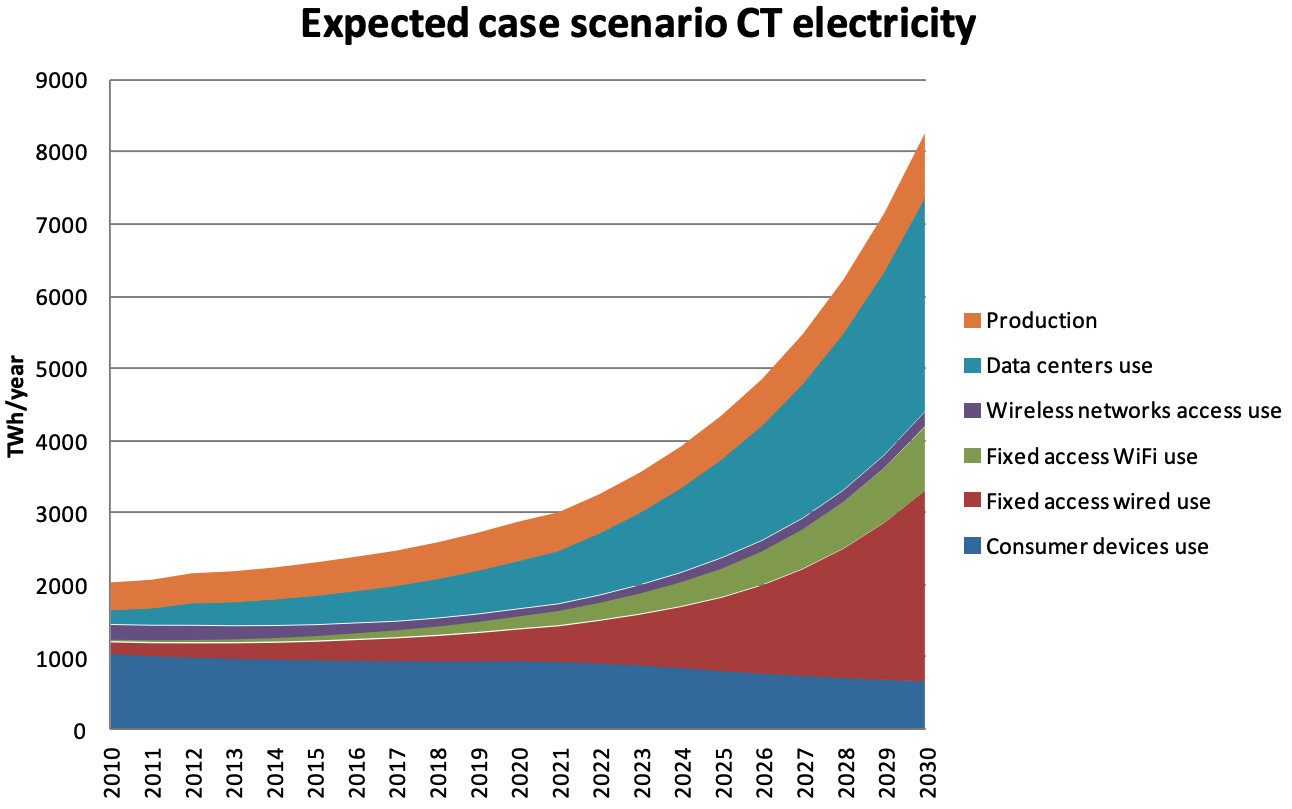
\includegraphics[width=.8 \textwidth]{./images/Global_Energy_ICT_components.png}
    \centering
    \caption{Trends per communication technology (CT) category for expected-case global electricity usage from 2010–2030. The fixed access network (FAN) usage is further broken down into the fixed access wired (red) and fixed access Wi-Fi (green) data traffic. The wireless access networks (WAN, purple) is based on the annual growth of voice traffic and mobile data traffic \cite{andrae2015global}.}
    \label{Global_Energy_ICT_components}
\end{figure}

\begin{figure}[h]
    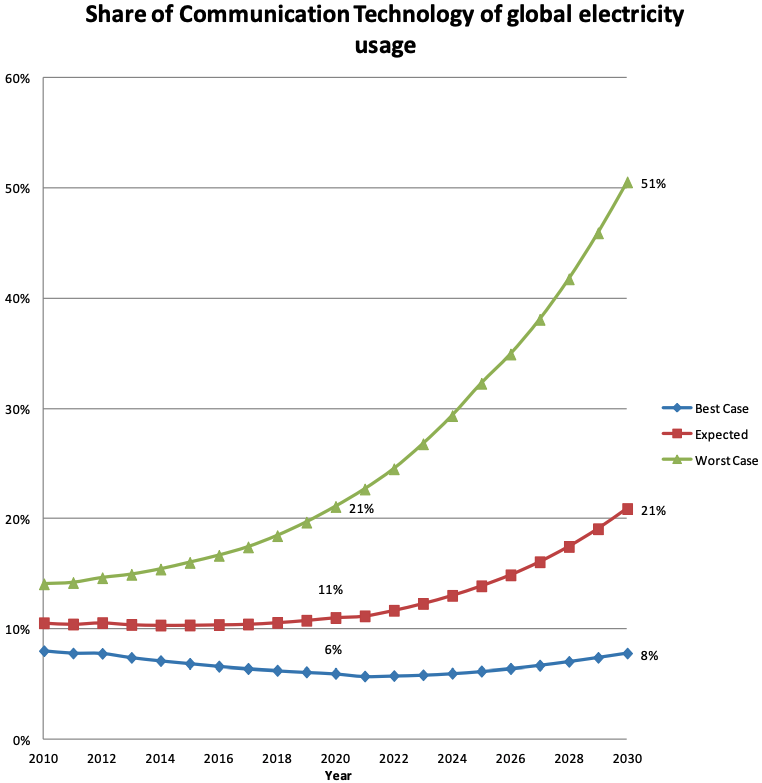
\includegraphics[width=.7 \textwidth]{./images/Global_Energy_ICT_share.png}
    \centering
    \caption{Share of communication technology of global electricity usage 2010–2030 \cite{andrae2015global}.}
    \label{Global_Energy_ICT_share}
\end{figure}

Although many ICT devices are now more energy efficient (for example, television panels have now transitioned to Light Emitting Display (LED) based displays \cite{park2013efficiency}), some newer models use substantially more energy. In November 2020, both Sony and Microsoft released their next-generation home consoles---the Playstation 5 (PS5), the Xbox Series X and the Xbox Series S---which were their most successful launches ever for both companies \cite{cnet2020gamingconsoles}. While they give an unprecedented gaming experience of speed, power, and graphics, they are also the most energy-intensive gaming consoles ever made (Figure \ref{usage_gaming_consoles}). For an in-depth life cycle analysis of gaming consoles, please see \cite{aslan2020climate}.

\begin{figure}[h]
    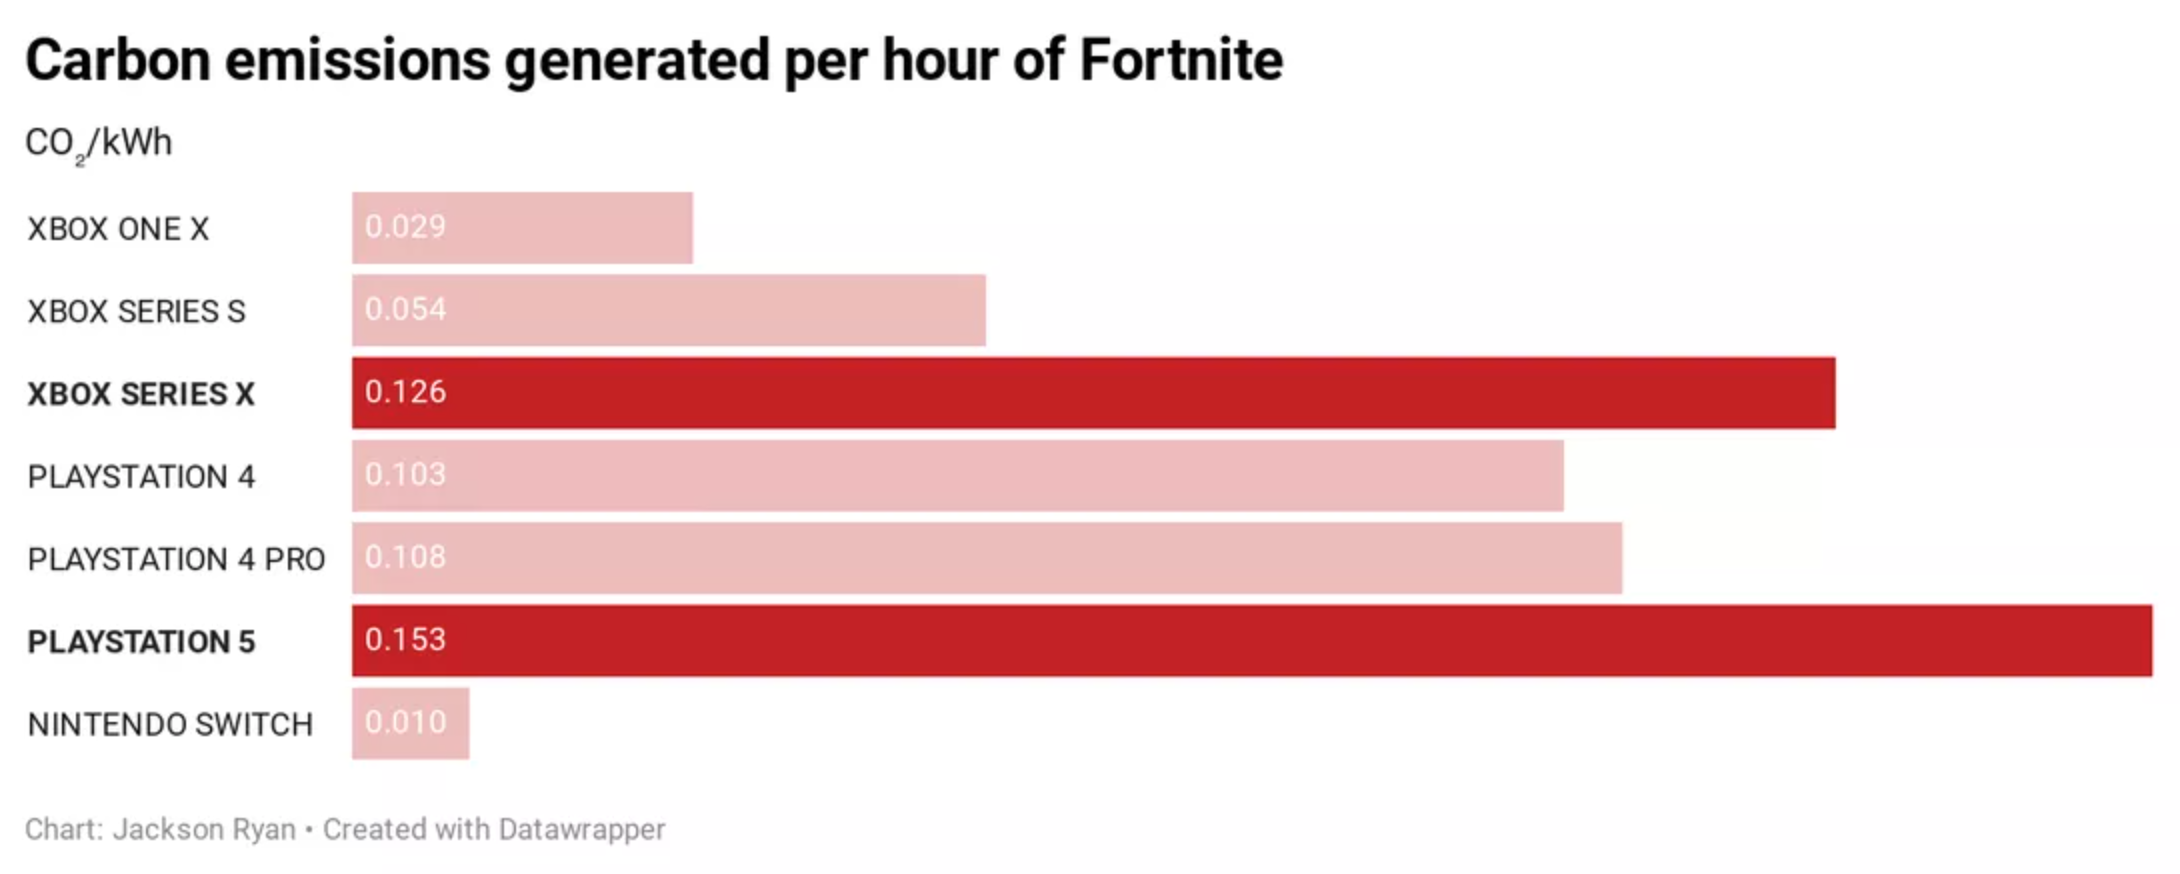
\includegraphics[width=.9 \textwidth]{./images/usage_gaming_consoles.png}
    \centering
    \caption{Comparison of the energy consumption for the newest generation (Playstation 5, Xbox Series X and Xbox Series S) versus the older generations of gaming consoles for a popular game. Note that the new Xbox Series S is the more affordable and less powerful alternative to the Xbox Series X \cite{cnet2020gamingconsoles}.}
    \label{usage_gaming_consoles}
\end{figure}


%%%%%%%%%%%%%%%%%%%%%%%%% Orwellian Energy %%%%%%%%%%%%%%%%%%%%%%%%%%%%%
\cleardoublepage
\subsubsection{Some Energy are More Equal Than Others}
While it is important to measure how much energy a device actually consumes, it is also crucial to examine how your energy is generated. Depending on whether your energy resources are coming from fossil fuels (coal, oil and natural gas), uranium, renewables (solar, wind, hydro), waste (for example, waste-to-energy incineration facilities), and/or biomass fuels, the environmental impacts will vary \cite{dincer2000renewable}. Even within a certain category of energy, there is substantial variation \cite{boyle2004renewable}.

A good illustration of this is a study conducted on the operational energy usage of Sweden's ICT network for a single year \cite{malmodin2014life}. In Figure \ref{usage_sweden_global_mix}, we see the carbon footprint of the extended Swedish ICT network is substantially less if computed using Sweden's energy mix (B) versus the same network being powered by the less clean global average electricity mix (C).

\begin{figure}[h]
    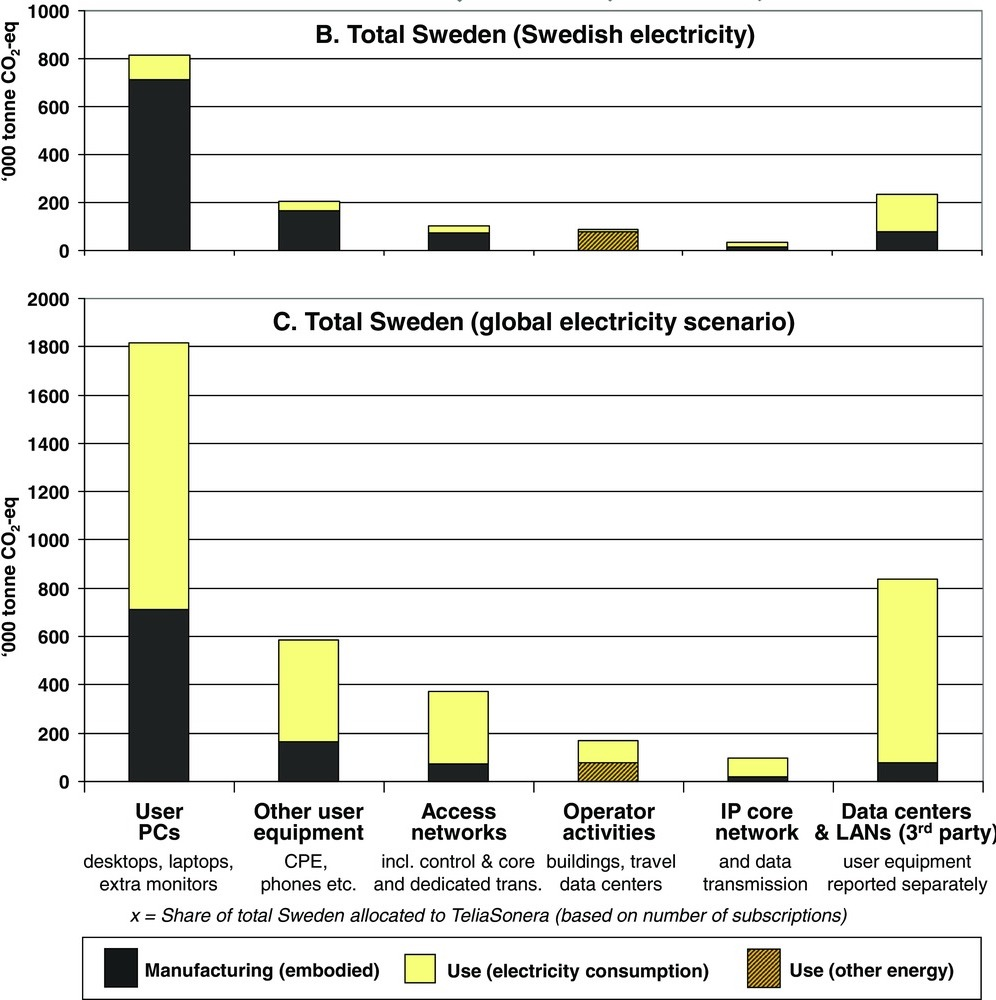
\includegraphics[width=.76 \textwidth]{./images/usage_sweden_global_mix.jpeg}
    \centering
    \caption{Carbon footprint of \textbf{(B)} the Swedish ICT extended network using the Swedish energy mix; and \textbf{(C)} the Swedish ICT extended network using a global energy mix. The carbon footprint is measured in units of carbon dioxide equivalent (CO$_2$-eq). Other acronyms used include Internet Protocol (IP), local area network (LAN) and customer premises equipment (CPE) \cite{malmodin2014life}.}
    \label{usage_sweden_global_mix}
\end{figure}

Although beyond the scope of this paper, if you are interested in the feasibility of providing all worldwide energy from wind, water, and solar (WWS) renewables, please see the two part series of \cite{jacobson2011providing, delucchi2011providing}. Interestingly, barriers to covert all power worldwide to WWS renewables are primarily social and political, not technological or even economic.


%%%%%%%%%%%%%%%%%%%%%%%%%%%%%%%%%%%%%%%%%%%%%%%%%%%%%%%%%%%%%%%%%%%%%%%%
%%%%%%%%%%%%%%%%%%%%%%%%% Lifespan of ICT  %%%%%%%%%%%%%%%%%%%%%%%%%%%%%
\subsection{The Lifespan of an ICT Device}
% Gadget Today, Garbage Tomorrow
So far we have examined the embodied emissions and the complex geopolitical implications of producing your device, the emissions to get the product into your hand and the energy consumed for the usage of your ICT device. Another important factor of the ICT footprint is how long we can use an ICT device before it truly is trash. A longer lifespan would reduce the total embodied and end-of-life emissions for the global ICT sector; a shorter lifespan means more raw materials are required, more devices must be manufactured and more devices must be disposed of or recycled. 

Unfortunately people often upgrade their ICT devices before their actual lifespan (Figure \ref{estimated_lifespan_ICT}). Despite mobile phones being designed to last at least 7 years, the average American changes their mobile phone every year while the average European does so every 18 months \cite{bournay2006vital, webfx2016lifespanICT}. These ex-marvels of technology are still functioning but they are often pre-maturely disposed of or lying around unused. Sometimes the discrepancy between actual versus theoretical lifespan arises from unforeseen circumstances that a company did not anticipate. But more often it is due to a deliberate effort by companies to ``[instill] in the buyer the desire to own something a little newer, a little better, a little sooner than necessary" \cite{stevens1960planned}.

\begin{figure}[h]
    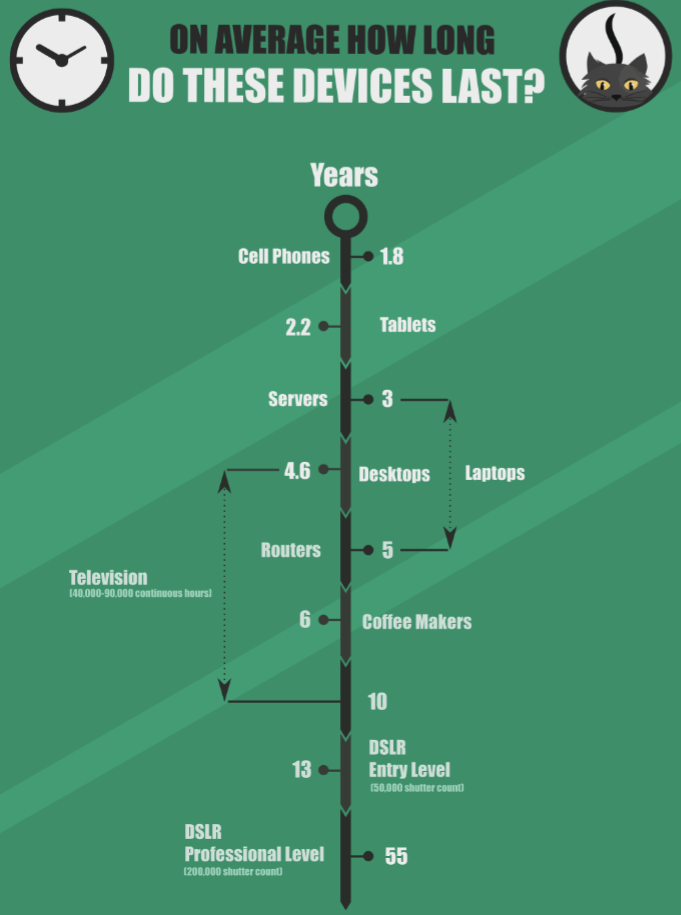
\includegraphics[width=.7 \textwidth]{./images/lifespan_ICT_US.png}
    \centering
    \caption{The estimated lifespan of common electrical and ICT devices in the United States of America \cite{webfx2016lifespanICT}.}
    \label{estimated_lifespan_ICT}
\end{figure}


%%%%%%%%%%%%%%%%%%%%%%%% Planned Obsolescence %%%%%%%%%%%%%%%%%%%%%%%%%%
\subsubsection{Planned Obsolescence} \label{SECTION_PLANNED_OBSOLESCCENCE}
Planned obsolescence is the production of goods with uneconomically short useful lives so that customers will have to make repeat purchases
\cite{bulow1986economic}. This is neither a new phenomena nor one only within the high technology industry: firms have an economic incentive to introduce new products that make their old products obsolete in order to stimulate replacement buying by consumers. This can be achieved through a number of \textit{physical obsolescence} mechanisms: limited functional life design (``death dating"), designing for limited repair (lack of affordable repair options or access to replacement parts), and design aesthetics that lead to reduced satisfaction (for example, a pristine and polished initial appearance that with everyday use will quickly become damaged, engendering user dissatisfaction and premature disposal) \cite{guiltinan2009creative}. A classic example of this mechanism is Apple product batteries: they are not removable by a customer and have a purposefully short lifespan. Since the product can only be fixed by Apple, they can charge sufficiently high repair prices so that it makes more sense for a customer to buy a new product instead of replacing the battery \cite{keeble2013culture}.

Even faster replacement can be achieved by fostering \textit{technological obsolescence}. This is achieved by designing a functional enhancement that adds or upgrades product features. Sometimes these are revolutionary (for example, adding a camera feature to a cell phone), but often they are the near constant progression of technology (making new laptops with increased memory or reduced weight) \cite{guiltinan2009creative}. This is a common practice amongst mobile phone companies, whom typically release a new model or updated model every year. It also coincides with the year or two update of a mobile phone contract, which allows people to get the latest phone on the market. There is a large psychological aspect to this phenomenon, which is covered in depth in \cite{keeble2013culture}. 

With \textit{style obsolescence}, a product becomes less fashionable and unwanted when a newer trend comes out. Consumers here are motivated by aesthetic considerations or by the implications in relation to their identity construction. Often the product is functional and working in every way other than aesthetics but since the product is no longer `in style' it will be replaced. Another technique of planned obsolescence is \textit{postponement obsolescence}. A company has technology that can be added to all of their products, but instead they choose to add only the best technology to their flagship product while the cheaper models have their second rate technology. Within a few years the flagship models will have even newer technology and so the the lower end models will typically have the flagship model's technology from years past \cite{keeble2013culture}.

In contrast, durable goods producers face a challenge in maintaining a high rate of sales growth: the more reliable and long-lasting the product, the longer the repeat purchase cycle and the slower the rate of sales growth. Durability also causes a greater competition between new and used versions. This creates an opportunity for a used market which will cause a decrease in price of the next generation of replacement products \cite{guiltinan2009creative}. In many places, the cost of product disposal is externalized to the community and so it is not a real cost to the producer. We could ask firms to voluntarily pay for their disposal or to reduce the rate at which new product improvements are brought to market, but this would be akin to requesting unilateral competitive disarmament \cite{guiltinan2009creative}. The literature on this social dilemma and public policy initiatives for planned obsolescence of ICT devices was rather sparse, but we will briefly discuss the growing global movement for citizens to have the right to repair their products.


%%%%%%%%%%%%%%%%%%%%%%% Right to Repair %%%%%%%%%%%%%%%%%%%%%%%%%%%%%%%%
\subsubsection{The Right To Repair}\label{SECTION_RIGHT_TO_REPAIR}
A straightforward way to extend an ICT device's life is to maintain, repair or refurbish it \cite{zerowastecanada2017hierarchy}. Unfortunately, this is not always an option for consumers. As of 2021 in the European Union, four types of electrical appliances (displays, washing machines, dishwashers and fridges) have to be made more easily repairable and longer-lasting. Although a major step forward towards a universal Right to Repair, there are still many holes: this has a limited scope (no smartphones or laptops), it has restricted access of certain spare parts and repair manuals to professional repairers, a long delivery time of spare parts, and there is no requirement for manufactures to update software throughout the lifetime of a product \cite{EUrighttorepair2021}.

Despite strong support amongst Canadians, a bill that would give consumers the right to repair their ICT devices, appliances, and vehicles was voted down in 2019 \cite{CArighttorepair2020fail}. In 2021 a national bill has been introduced; it is not a true Right to Repair but instead a first step. At the time of writing, its fate is promising but it faces strong opposition from many companies, including John Deere (farm and construction equipment) and Apple \cite{CArighttorepair2021national}.


%%%%%%%%%%%%%%%%%%%%%%%%%%%%%%%%%%%%%%%%%%%%%%%%%%%%%%%%%%%%%%%%%%%%%%%%
%%%%%%%%%%%%%%%%%%%%%%% End-Of-Life Emissions %%%%%%%%%%%%%%%%%%%%%%%%%%
%%%%%%%%%%%%%%%%%%%%%%%%%%%%%%%%%%%%%%%%%%%%%%%%%%%%%%%%%%%%%%%%%%%%%%%%
\cleardoublepage
\section{End of Life Emissions} \label{SECTION_END_OF_LIFE_EMISSIONS}
 \begin{fquote}[Case Study from Heftingsdalen, Norway][Vital Waste Graphics 2 \cite{bournay2006vital}]
 For consumers, waste disappears the moment their bin is emptied. They see us as a sort of cemetery for the consumer society. They completely disregard the concept of waste and what it becomes. Nor do they have much idea of the many ways waste may be processed. Nothing disappears. It all becomes something else, which inevitably impacts on our environment and way of life...Five years ago waste processing plants represented a fairly effective, sustainable solution, now they are a crisis response.
 \end{fquote}


E-waste\footnote{E-waste is also known as Waste Electrical and Electronic Equipment (WEEE), a term mostly used in Europe. The e-waste statistics used in this section include ICT devices as well as other electronic and electrical equipment (e.g., basic kitchen appliances, toys, lamps, and tools for music).} are the electrical and electronic equipment (EEE) and its components that have been discarded as waste without any intention of reuse (Figure \ref{e-waste}). In 2019, the world generated an astounding 53.6 Mt\footnote{1 metric megaton (Mt) is equivalent to 1,000,000,000 kilogram (kg).} of e-waste, which averages to 7.3 kg per person). And this number is projected to increase with a doubling time of 16 years: by 2030, the world is projected to create 74.7 Mt of e-waste. This growth is not distributed equally, however. Although Asia generated the most amount of e-waste, per capita Europe is the highest with each citizen producing an average of 16.2 kg of e-waste. This is followed by similar levels in Oceania (16.1 kg per capita) and the Americas\footnote{Within certain regions, there is even more variation. For example, Northern America (Canada and the USA) produce 20.9 kg per capita and have a recycling rate of 15\%, whereas Central America (Mexico, Guatemala, Costa Rica) only produce 8.3 kg per capita with a recycling rate of 3\%.} (13.3 kg per capita). Asia and Africa have by far the lowest, with 5.6 and 2.5 kg per capita, respectively. For a comprehensive breakdown of global and regional e-waste statistics, legislation and health impacts, please see \cite{forti2020global}.

\begin{figure}[h]
    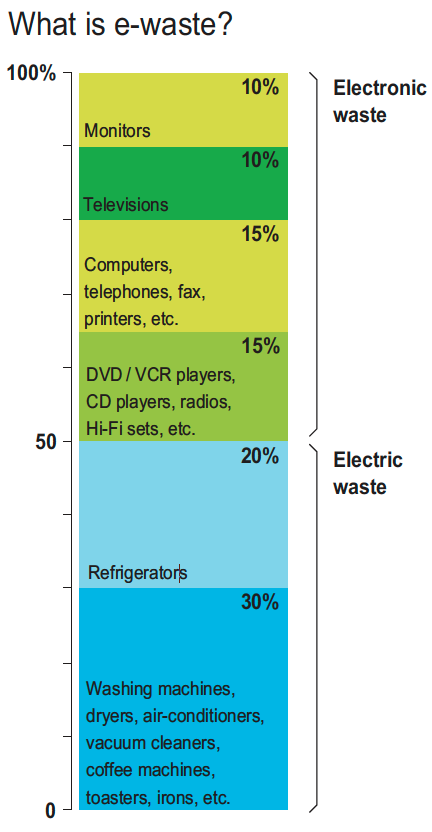
\includegraphics[width=.35 \textwidth]{./images/e-waste.png}
    \centering
    \caption{Components of e-waste. Additional categories not included in this infographic include: lighting equipment (fluorescent tubes); toys, sports and recreational equipment; electric and electronic tools (drills, sewing machines, lawn mowers, etc); surveillance and control equipment; medical instruments; and automatic ticket machines \cite{bournay2006vital}.}
    \label{e-waste}
\end{figure}

The major factors enabling this increased consumption of ICT devices globally are higher levels of disposable income, growing urbanization and mobility, and further industrialization (Section \ref{SECTION_WIDESPREAD_ADOPTION_OF_ICT}). In addition to this higher consumption rates of ICT devices, shorter product life cycles (Section \ref{SECTION_PLANNED_OBSOLESCCENCE}) and few repair options (Section \ref{SECTION_RIGHT_TO_REPAIR}) means that more of these devices are becoming e-waste sooner (Figure \ref{Global_e_waste_stats}). Since we discussed these factors contributing to e-waste in previous sections, please refer back to them if you require a refresher.

Much of this waste is classified as hazardous due to its component metals (Section \ref{SECTION_ACQUISITION_RAW_MATERIALS}), the use of brominanted flame retardants (BFRs) to improve fire safety, and the compounds generated or used during the recycling process \cite{williams2011environmental, forti2020global}. In addition to the valuable metals of copper, gold, and silver in an ICT device, you also have an assortment of hazardous metals including lead (soldering), antimony and arsenic (chip) \cite{compoundinterest2014, williams2011environmental}, mercury (background lights of older displays and televisions) \cite{balde2018waste}, cadmium (rechargeable batteries)  \cite{williams2011environmental, forti2020global} and lithium (lithium batteries) \cite{compoundinterest2014, kumar2017waste}.

\begin{figure}[h]
    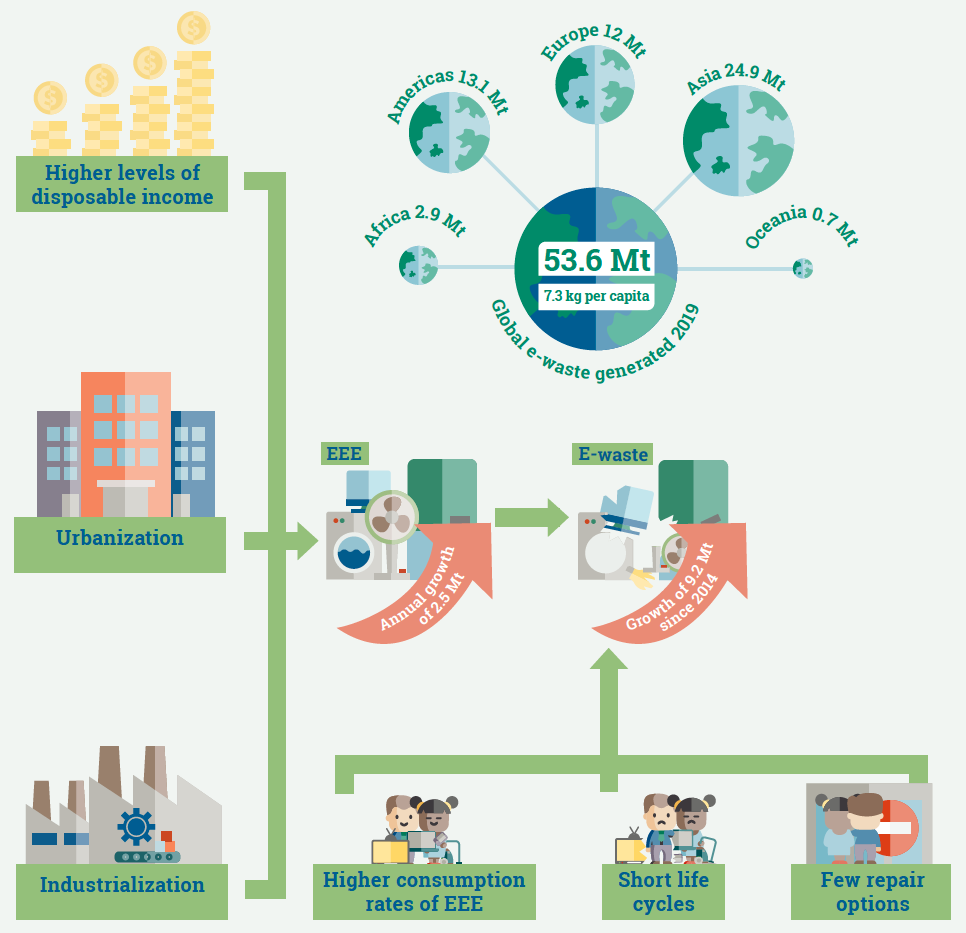
\includegraphics[width=.8 \textwidth]{./images/e-waste_global.png}
    \centering
    \caption{Global production of e-waste broken down by regions, as well as the major contributing factors for the growth of the electrical and electronic equipment (EEE) consumption and the growth of its subsequent e-waste \cite{forti2020global}.}
    \label{Global_e_waste_stats}
\end{figure}


%%%%%%%%%%%%%%%%%%%%%%%%%%%%%%%%%%%%%%%%%%%%%%%%%%%%%%%%%%%%%%%%%%%%%%%%
%%%%%%%%%%%%%%%%%%%%%%%%%%%%% Disposal %%%%%%%%%%%%%%%%%%%%%%%%%%%%%%%%%
\subsection{Disposal}
Not all discarded ICT devices will end up in recycling centres. The fate of 82.6\% (44.3 Mt) of generated e-waste in 2019 is unknown: we know neither its whereabouts nor do we know its environmental impacts. This is troubling because many abandoned devices contain hazardous elements that may leach into the environment \cite{forti2020global}. Mercury can enter the food chain and accumulate in living organisms, resulting in damage to the central nervous system, thyroid, kidneys, lungs, immune system and irreversibly brain damage \cite{balde2018waste}. Unfortunately, this improper management of e-waste results in a sizeable amount of raw materials not being recovered \cite{forti2020global}. These lost raw materials in e-waste cannot be used to substitute primary raw materials and so we require even more extraction and refinement of virgin material deposits (Section \ref{SECTION_ACQUISITION_RAW_MATERIALS}).


%%%%%%%%%%%%%%%%%%%%%%%%%%%%%%%%%%%%%%%%%%%%%%%%%%%%%%%%%%%%%%%%%%%%%%%%
%%%%%%%%%%%%%%%%%%%%%%%%%%%%% Recycling %%%%%%%%%%%%%%%%%%%%%%%%%%%%%%%%
\subsection{Recycling}
Although the majority of e-waste is unaccounted for, globally we collected and recycled 17.4\% of e-waste in 2019. Similar to the generation of e-waste, the recycling rates are not evenly distributed across the globe. In 2019, Europe had the highest rate at 42.5\%, followed by Asia (11.7\%), the Americas (9.4\%), Oceania (8.8\%), and Africa (0.9\%) \cite{forti2020global}.

% Part 1: Recycling Rates
\subsubsection{How Recyclable are My Recyclables?}
Let's say you are one of the lucky ICT devices that does make it to a (formal or informal) recycling center. Even if an ICT device is recycled, there is a significant variation between the recycling rates of each metal (Figure \ref{Recycling_Rates_Smartphone}). In the case of rare earth elements, you have a less than 1\% recycling rate; often it is not economically possible to retrieve these trace metals because the amounts used are so small \cite{physorg2012scarcemetals, habib2015tracking}. And so we risk irretrievable dissipation of these already scarce elements into the biosphere, rendering them impossible for reuse \cite{reller2009mobile}. Although the scarce metal cobalt has a $>50\%$ recycling rate, the remaining scarce metals of indium, tantalum and all of the rare earth elements have a $<1\%$ recycling rate \cite{compoundinterest2014}. Within 1 tonne\footnote{1 tonne is equivalent to 1,000 kilograms or 1,000,000 grams.} of mobiles phones, there are 280 grams of gold \cite{forti2020global} (in comparison, the gold ore grade is approximately 5 grams of gold per 1 tonne of ore) \cite{mudd2007sustainability}. Since newer phones are being manufactured with less gold, they require less raw materials. Unfortunately they are now less profitable to recycle and so the gold contained within them is often not recovered \cite{geyer2010economics}. For the plastic components, the outlook is not much better. Of the seven billion tonnes of plastic waste that humanity has generated so far, an estimated 10\% were recycled and 14\% were incinerated, while the remaining 76\% are either in landfills, dumps, or the natural environment \cite{geyer2020production}. These poor recycling rates unfortunately puts additional stress on supply chains.

\begin{figure}[h]
    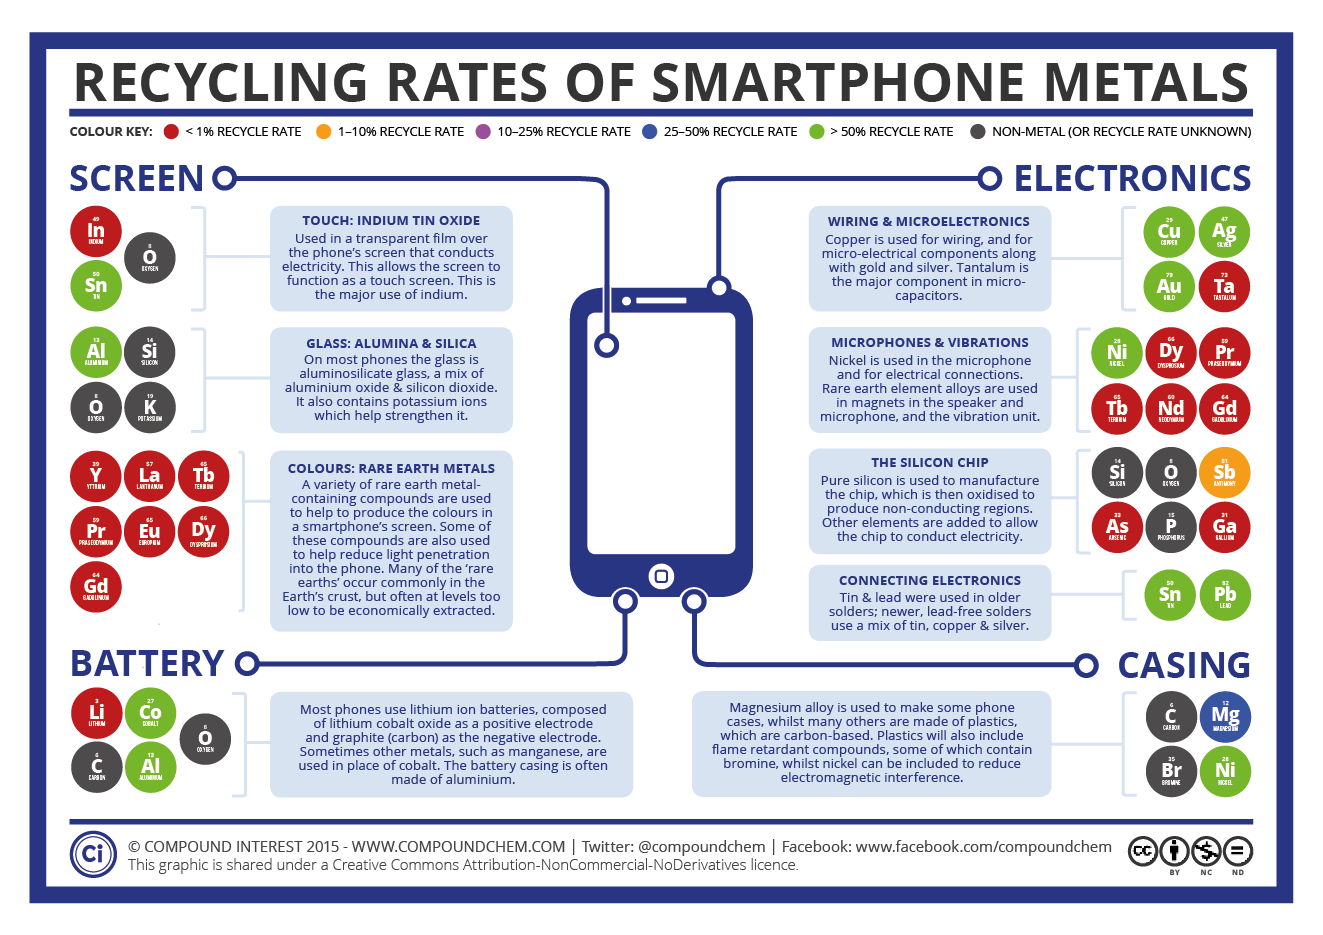
\includegraphics[width=1 \textwidth]{./images/recycling_rates_of_smartphone.png}
    \centering
    \caption{Recycling rates of a smartphone, broken down by its screen, electronics, battery and casing \cite{compoundinterest2014}.}
    \label{Recycling_Rates_Smartphone}
\end{figure}

Let's say you are also one of the lucky percentages that did get recycled. There is still another obstacle you may face on your path to being truly recyclable: the vast majority of recycling today is actually downcycling. When a material is recycled, they are often mixed with other materials to produce a hybrid of lower quality therefore making them suitable only for applications of lower value. Rather than creating a circular cradle-to-grave dynamic, their trip to the landfill has only been slowed. This is problematic for metals since the rare earth elements and valuable minerals are blended in the recycling process, thus making their discrete value lost forever \cite{braungart2007cradle}. Downcycling is also problematic for plastics which make up approximately 50\% of a smartphone, most of which is contained in the case and circuit boards \cite{bournay2006vital}.

When recycling, it is often difficult to separate the hazardous wastes from the valuable material. An example of this are the brominanted flame retardants found in the outer casings of computers, circuit boards, wires and cables in order to improve fire safety \cite{williams2011environmental, forti2020global}. When this e-waste is recycled into waste plastic it can then be used in lower grade applications, including plastic kitchen equipment. Despite European legislation prohibiting BFRs in food contact articles, studies have shown that BFRs are present in black thermos cups and black plastic kitchen utensils \cite{samsonek2013occurrence}.


%%%%%%%%%%%%%%%%%%%%%% Waste Colonialism %%%%%%%%%%%%%%%%%%%%%%%%%%%%%%%
\subsubsection{Not in My Backyard}
% This also got me thinking about waste colonialism —it’s a concept that describes the transboundary movement of waste largely overseas transferring waste and its burdens from high GDP nations to low GDP nations -- not only does the Global North place the blame on marginalized individuals but also the burdens

Unwanted ICT products may still be refurbished and reused and so they are often shipped from higher income countries to lower income countries, which may or many not have a fully developed e-waste management infrastructure. Although some ICT devices extend their life cycle this way, a sizeable amount of e-waste generated is illegally shipped under this guise \cite{forti2020global}. %Despite having e-waste recycling infrastructure, high-income countries export a sizeable portion to developing countries. 

The 1970s and 1980s saw a rise of environmental regulations to properly handle hazardous wastes in developed countries, resulting in a higher cost for e-waste disposal. In developing countries  there are fewer safety regulations, lower cost of labour and a strong demand for raw materials in transitioning economies. Since developed countries could no longer dump their unwanted hazardous materials in a local landfill, it became more economical for them to load these wastes onto ships and trains, transport them beyond their regulated jurisdictions and dump them in another backyard for a fee. The result was a massive trans-boundary flow of e-waste from developed countries to developing countries such as China, India and Pakistan  \cite{sthiannopkao2013handling, zhang2012waste}.

In response to this digital dumping situation, the 1992 Basel Convention on Transboundary of Movement of Hazardous Waste and their Disposal banned this toxic trade of hazardous wastes, including e-waste \cite{baselconvention2011}. Although a comprehensive agreement that charged countries to be responsible for the safe disposal of the hazardous wastes they produced, it did not extend to functioning second-hand goods \cite{sthiannopkao2013handling}. Despite China\footnote{Upon resuming sovereignty of Hong Kong, the Basel Convention also applied to the Hong Kong Special Administrative Region.} ratifying the Basel Convention in 1991 \cite{baselconvention2011ratify}, the illegal smuggling of e-waste continued to pour in. The New Territories region of Hong Kong is a major e-waste trafficking port; from here it is then smuggled across to mainland China \cite{ban2018carecyclingexport}. To stop the illegal export of waste from other countries, China began enforcing strict border controls in 2013 (Operation Green Fence) and even stricter measures in 2017 (National Sword). Although it successfully reduced the illegal waste accepted at the Chinese border, it had unfortunate cascading effects. Rather than developed countries reducing or processing all of their waste, the problem has been shifted to yet another backyard \cite{financialtimes2018nationalsword}. Much of the rejected waste has ended up in other Southeast Asian countries and Pakistan (Figure \ref{e-waste_china_import}), many of whom lack the infrastructure to manage their own waste, much less the additional waste from the developed world \cite{ban2018carecyclingexport, brooks2018chinese}.

\begin{figure}[h]
    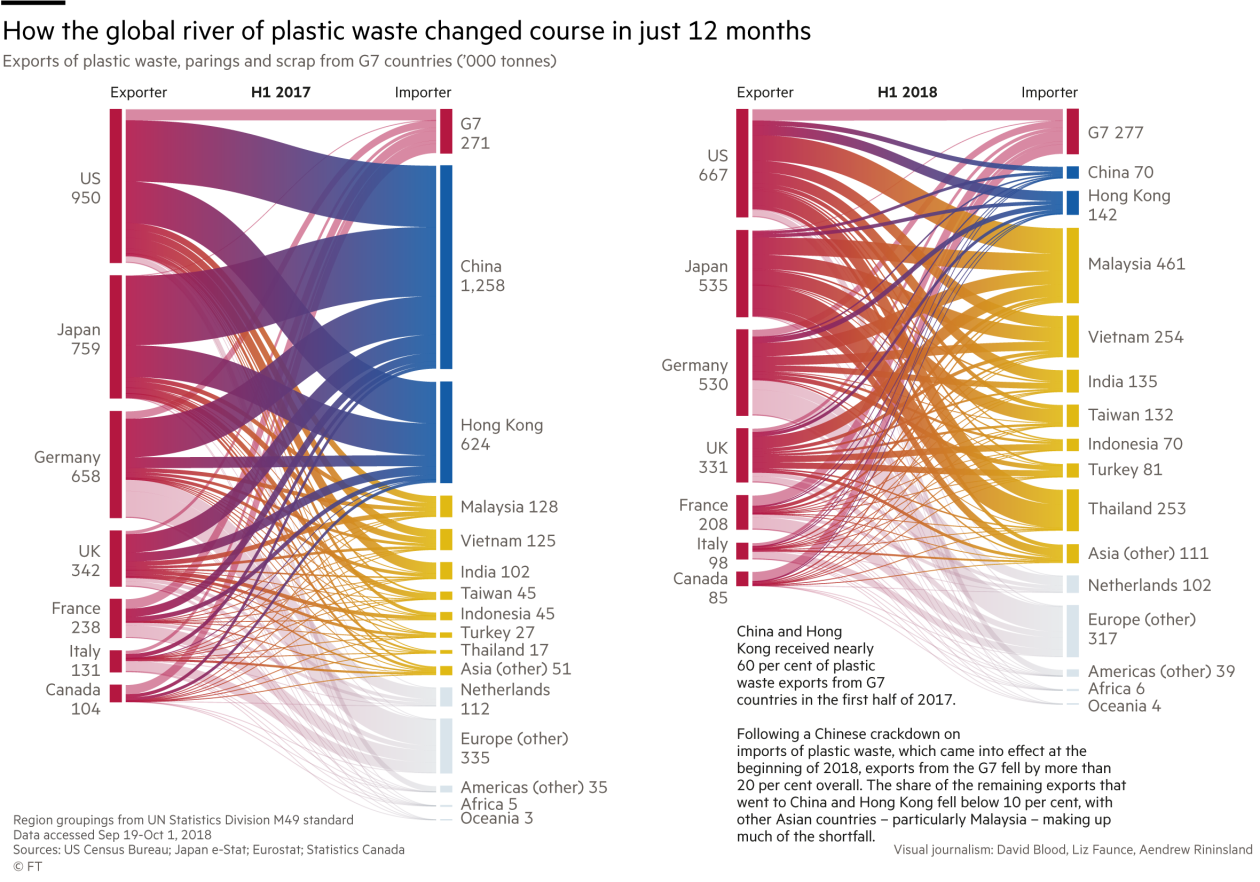
\includegraphics[width=.9 \textwidth]{./images/e-waste_china_import.png}
    \centering
    \caption{\textit{The import and export of plastic waste from G7 countries before and after China's National Sword \cite{financialtimes2018nationalsword}.}}
    \label{e-waste_china_import}
\end{figure}

A 2016 study using Global Positioning System (GPS) trackers found that 34\% of the USA's e-waste were exported, with the majority going to Hong Kong (Figure \ref{US_export_e-waste}) \cite{ban2016usrecyclingexport}. A similar 2018 study in Canada found a 16\% export rate of recyclers \cite{ban2018carecyclingexport}. Although better, it is still concerning since Canada has a legal obligation under the Basel Convention, while the USA does not \cite{baselconvention2011ratify}. 

\begin{figure}[h]
    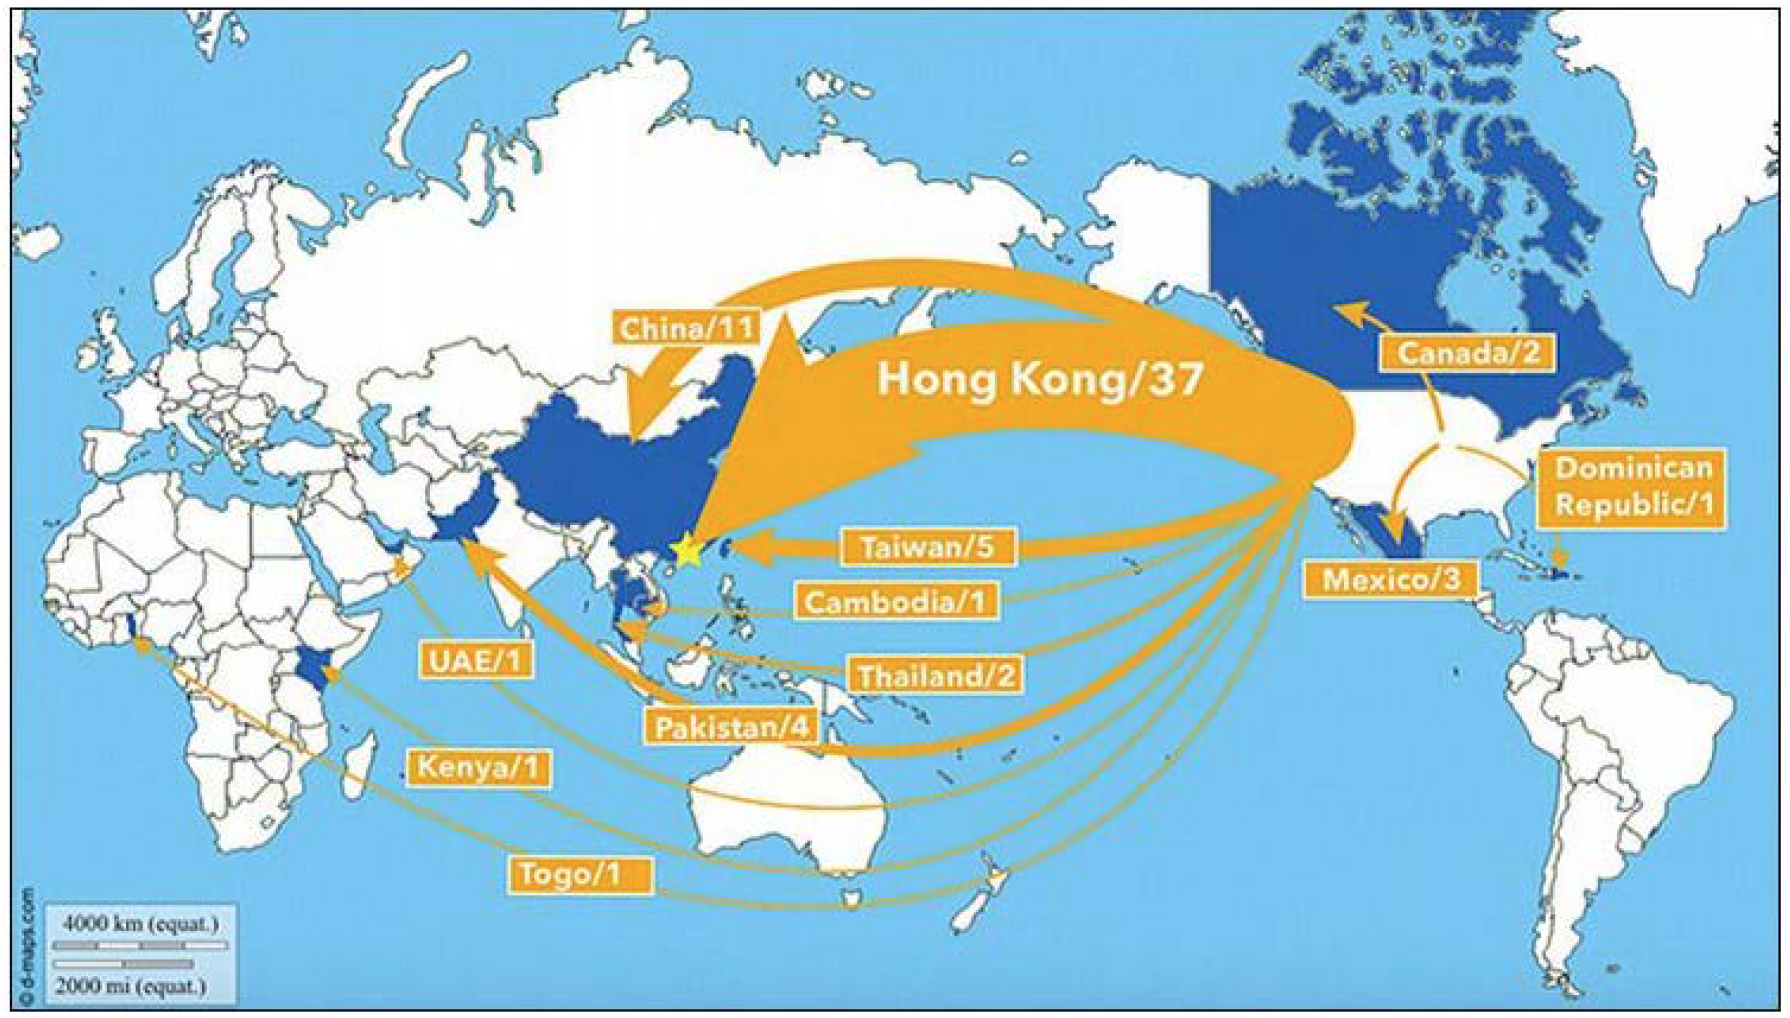
\includegraphics[width=.8 \textwidth]{./images/US_export_e-waste.png}
    \centering
    \caption{A map showing the destinations of the electronic products tagged with trackers in the e-Trash Transparency Project \cite{ban2016usrecyclingexport}.}
    \label{US_export_e-waste}
\end{figure}

When we throw our waste ``away", away becomes ``here" for someone else. A framework for viewing this transboundary movement is \textit{waste colonialism}: developed nations use their dominance (or hegemonic power) to exploit the land of developing nations for waste disposal. Blame is then attributed to developing nations' poorer waste disposal systems and international emissions accounting reinforces this by allowing developed nations to export their e-waste emissions (Section \ref{SECTION_RESPONSIBILITY_OF_EMISSIONS}). Consequences of waste pollution disproportionately impact those who are least responsible for the pollution and who are least able to mitigate the effects \cite{liboiron2018plastic, pratt2010decreasing}.


%%%%%%%%%%%%%%%%%%%%%%%%%%% Formal Recycling %%%%%%%%%%%%%%%%%%%%%%%%%%%
\cleardoublepage
\subsubsection{The Formal Recycling Sector}

The formal recycling sector is typically established by national e-waste legislation. E-waste is collected by designated organizations, producers, or the government (often through retailers, collection points or pick-up services) and it is taken to specialized treatment facilities \cite{forti2020global}. In the first step, hazardous materials are separated from electronic devices, which are further dismantled into their plastic, glass, wires and electrical components. During the end-processing stage, the wires and electronics are sent to a smelter to recover the valuable metals which are then purified in refineries \cite{kumar2017waste}. Meanwhile the plastic components are melted down for re-use in lesser applications, in a process known as downcycling \cite{braungart2007cradle}. Wastes from this process are either incinerated or held in controlled landfills. This formal recycling process should be performed in accordance to the country's e-waste legislation, which typically mandates the proper handling of hazardous wastes and protection of the health of workers and the environment \cite{forti2020global}. Despite these health and safety regulations, damage to the environment, the health of the workers and surrounding populations are still an issue (Section \ref{SECTION_RECYCLE_ENVR_IMPACTS}).

Although higher-income countries tend to have a waste recycling infrastructure, around 8\% of e-waste still ends up in waste bins and is subsequently incinerated or placed in landfills. Consequently this e-waste is treated like regular mixed household wastes. These are typically incinerated or landfilled without material recycling or the safe handling of hazardous elements \cite{forti2020global}. 


%%%%%%%%%%%%%%%%%%%%%%% Informal Recycling %%%%%%%%%%%%%%%%%%%%%%%%%%%%%
\subsubsection{The Informal Recycling Sector}
Since many middle- and low-income countries have an e-waste management infrastructure that is not fully developed or entirely absent, e-waste is often managed by the informal sector. The informal sector is typically characterized by small-scale, labour-intensive, low-technology recycling that is unregulated and unregistered. It is often carried out by poor and marginalised social groups who must resort to scavenging and waste picking in order to generate income---sometimes for everyday survival. Although informal recycling is typically regarded in a very negative light, %---it is backward, unhygienic and incompatible with modern waste management systems---
it is a rather efficient recycling system that can improve recycling rates and it provides a livelihood for a major section of the urban poor \cite{wilson2006role, medina2000scavenger}.

The collection phase of used products and e-waste can be identified into at least four main categories: 1) door-to-door buying, bartering or collecting; 2) street waste picking from litter or communal bins before collection; 3) municipal waste collection crews recovering materials from the vehicles on the way to disposal sites; and 4) waste picking from dump sites \cite{wilson2006role}. Once collected, the products are sold to be repaired, refurbished or informally recycled. Within the recycling phase, dismantlers manually break the e-waste into usable components and materials, using simple tools or their bare hands. For components that are no longer functioning but still contain valuable materials, recyclers will burn, leach and melt the e-waste to recover the secondary raw materials \cite{forti2020global}. Since they are encased by a plastic cover, cables are openly burnt to remove the plastic and recover the valuable copper. This is usually done a short distance from where the dismantling is performed due to the toxic smoke generated \cite{akormedi2013working}. Similarly, computer casings are ``cooked" to remove the combustible plastics and to isolate the metals. To release the chips, circuit boards are de-soldered by grilling them over an open fire to melt the lead and plastic. Once released, the chips are placed in open-pit acid baths to leach the gold and other metals. These wastes may then be directly disposed into nearby fields, rivers and irrigation ditches \cite{chan2013review, sthiannopkao2013handling}. This lack of safety regulations and equipment exasperates the challenges of recycling, causing severe damage to the environment and the health of the workers and surrounding populations (Section \ref{SECTION_RECYCLE_ENVR_IMPACTS}).

\begin{figure}[h]
    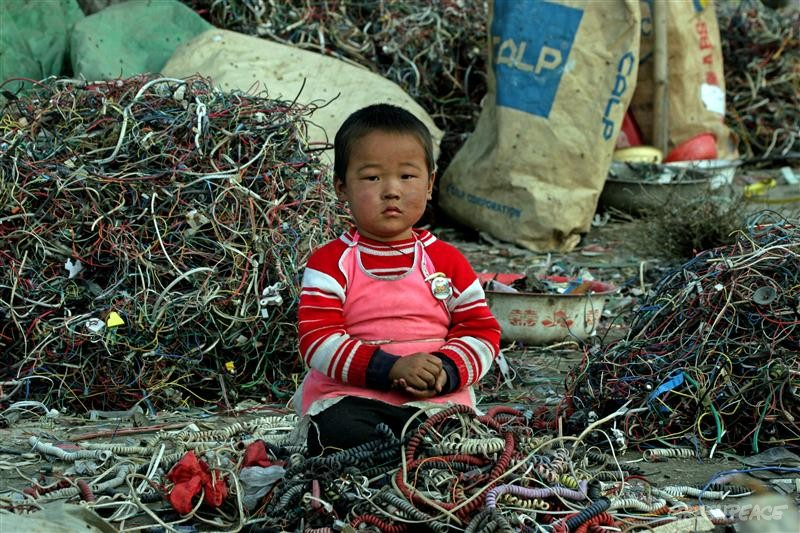
\includegraphics[width=.9 \textwidth]{./images/e-waste_guiyu.png}
    \centering
    \caption{A small child sitting among cables and e-waste in the informal recycling sector in Guiyu, China \cite{greenpeace2005guiyuewaste}.}
    \label{guiyu_e-waste}
\end{figure}

One of the most notorious case studies of informal recycling is the town of Guiyu in southeast China which processed over 20 million tonnes of e-waste in 2004 alone. There were more than 5,500 shops informally employing over 30,000 people, many of whom were children, for an average wage equivalent of US\$1.50 per day \cite{chi2011informal, chan2013review}. Most workers laboured without goggles, proper ventilation or other basic personal protective equipment \cite{sthiannopkao2013handling}. In 2015, China closed down Guiyu's informal sector and forced all e-waste processors in the area to either quit or relocate to the new industrial park. Although a major step for enforcing China's e-waste importation ban and improving the local environmental and human health, e-waste smugglers have simply found new backyards to dump their e-waste to be informally processed. Shortly after, concerns began to arise over the New Territories in Hong Kong being the next Guiyu \cite{ban2018carecyclingexport}.


%%%%%%%%%%%%%%%%%%%  Human & Environmental Impacts %%%%%%%%%%%%%%%%%%%%%
\subsubsection{Environmental \& Human Health}\label{SECTION_RECYCLE_ENVR_IMPACTS}

%%%%%%%% Informal %%%%%%
Many hazardous compounds enter the surrounding ecosystem by direct dumping into water systems, fumes and dust entering the atmosphere and soil, and the leaching of substances from landfills, incinerators and recycling \cite{williams2011environmental}. From here they may enter the water and food systems through the livestock, fish and crops (Figure \ref{e-waste_ecosystem_contamination}). Although workers---especially those without personal protective equipment---have direct exposure, the surrounding community will still be exposed through dietary intake, soil and dust ingestion, inhalation and dernal contact  \cite{williams2011environmental, chan2013review}. Unregulated e-waste recycling has been associated with a myriad of adverse human health effects, including prenatal exposure causing adverse birth outcomes \cite{xu2012birth}, limited or delayed growth and development of children \cite{liu2018thyroid}, decreased learning outcomes \cite{soetrisno2020chronic}, damaged DNA \cite{alabi2012comparative}, changes to cardiovascular regulation \cite{cong2018elevated}, decline in lung function and an increased risk for asthma and chronic obstructive pulmonary disease (COPD) \cite{amoabeng2020effect}, weakened immune systems \cite{zhang2017alteration}, hearing loss \cite{xu2020hearing}, and cancer \cite{davis2019strong}.

\begin{figure}[h]
    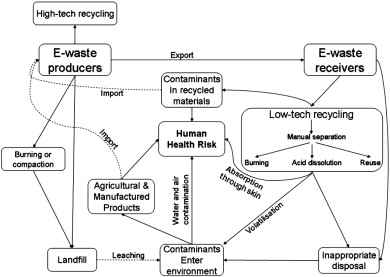
\includegraphics[width=.8 \textwidth]{./images/e-waste_ecosystem_contamination.jpg}
    \centering
    \caption{Exposure routes and behaviour of e-waste toxicants from producers to receivers and ultimately to humans \cite{robinson2009waste}.}
    \label{e-waste_ecosystem_contamination}
\end{figure}

%%%%%%%%% Formal %%%%%%%%%
Although the formal sector has safety regulations and protective equipment for workers, the concentration of hazardous compounds and exposure is still adverse for workers and the surrounding community. In a study of Canadian e-waste workers, certain air concentrations, dust concentrations, and worker exposures in formal indoor facilities exceeded those of informal indoor e-waste facilities in low and middle income countries. Possible explanations included the facilities being contained in a large but enclosed indoor facility (which had minimal natural ventilation) and a lack of operating emission abatement equipment \cite{nguyen2019exposure, nguyen2020can}. Workers performing recycling tasks in Sweden's formal e-waste facilities had significantly higher concentrations of toxic metals including chromium, cobalt, indium, lead, and mercury \cite{julander2014formal}. Community exposure is also a problem for the towns surrounding formal recycling facilities. The Horne smelter in Canada is North America's largest recycler of electronic components and is one of the world's largest producers of copper and other precious metals. To the residents' surprise, it was announced at a 2019 town hall meeting that the lead and arsenic levels in their children were 3.7 times higher than children living in a nearby town. In response, the company owning the smelter has added more domes to manipulate the process within a closed environment instead of outdoors; there was no comment on the impact of this on indoor air concentrations, dust concentrations or worker exposure. According to the federal database of pollutants, the Horne Smelter has released 936,000 kg of arsenic and 2,710,000 kg of lead since 1993 \cite{cbc2019hornesmelter}.

%Children attending school within a 2.5 kilometers radius of a smelter had higher levels of lead within their blood. As well, lead in school-playground dust and lead on children's hands were correlated to the lead in the air \cite{roels1980exposure}.

%%%%%%%%%%%%%%%%%%%%%%%%%%%%%%%%%%%%%%%%%%%%%%%%%%%%%%%%%%%%%%%%%%%%%%%%
%%%%%%%%%%%%%%%%%%%%%%%% Legislative Solutions %%%%%%%%%%%%%%%%%%%%%%%%%
\subsection{Searching for Solutions}

\begin{fquote}[Dr. Max Liboiron][How Plastic Is a Function of Colonialism \cite{liboiron2018plastic}]
Disposability is not the result of the bad behavior of some individuals choosing to buy some things and not others. Consumer choice as a concept makes no sense in many places. In Nain [the most northern Inuit community in Nunatsiavut, Canda], there is one store. There is one kind of ketchup you can buy. There is one type of lettuce. Both are in plastic packaging because the producers assume that there is a place for that packaging to go. It goes into the dump, where it is usually burned so bears aren't attracted to town, and then the scraps blow into the water. There is no way to behave differently. Bag bans don't eliminate the problem. Degradable plastics made of corn would move the problem onto someone else's land. Shipping Nain's plastics to a recycling plant in Vietnam or even elsewhere in Canada produces pollution and plastic leakage on other lands still. Disposable plastics are simply not possible without colonizer access to land.
\end{fquote}


%%%%%%%%%%%%%%%%%%%%%%%%%%%% Rethink %%%%%%%%%%%%%%%%%%%%%%%%%%%%%%%%%%%
\subsubsection*{\textit{Rethink}}
Rather than band-aid solutions that temporarily mask our e-waste problems, we need to take a systematic approach by rethinking our current processes, policies and actions to make meaningful change \cite{zerowastecanada2017hierarchy}. At this highest level of the Zero Waste Hierarchy (Figure \ref{zero_waste_hierarchy}), we need to make fundamental changes to our product designs. For example, we could design our ICT products for disassembly and easy separation, use single rather than composite materials and coatings, and expand product manufacturer's responsibility to include the full life cycle of their products (also known as extended producer responsibility). By providing incentives for manufacturers to design products that are easier to recycle, reuse and have reduced material usage, the environmental impact of a product across its life cycle can be reduced \cite{walls2006extended}.

\begin{figure}[h]
    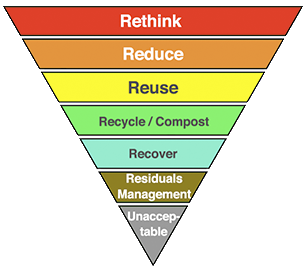
\includegraphics[width=.5\textwidth]{./images/zero_waste_hierarchy_crop.png}
    \centering
    \caption{Canada's Zero Waste Hierarchy \cite{zerowastecanada2017hierarchy}.}
    \label{zero_waste_hierarchy}
\end{figure}

On an individual consumer level, we can also rethink how we choose the ICT devices that we buy. Rather than purchasing ICT devices based on the more typical metrics of initial costs or the latest trends, you could also base your decision on other metrics (circumstances permitting). Other potential factors to consider are the device's embodied emissions, its lifespan, durability, repairability, reusability, or multifunctionality. Not everyone will have the privilege to access or base their decisions on more long-term considerations \cite{boddy2016telling} nor does individual action at the end of the pipeline address the underlying systemic issues. As well, the rise of the conservation movement has a long history baked in privilege, power and racism; this is beyond the scope of the paper but if you are interested we strongly recommend reading further \cite{taylor2016rise, purdy2015environmentalracism}.


An interesting piece of research by \cite{ryen2014community} tried to examine what more green ICT design would look like. By adapting biological ecology models to analyze the dynamic structure and function of the ICT device community, future strategies to encourage more green design and consumption of ICT devices should focus on minimizing the total number of products. One way to achieve this is by maximizing each device's multifunctionality with convergent device design.


%%%%%%%%%%%%%%%%%%%%%%%%%% Reduce & Reuse %%%%%%%%%%%%%%%%%%%%%%%%%%%%%%
\subsubsection*{\textit{Reduce \& Reuse}}
We have previously discussed the proliferation of ICT devices (Section \ref{SECTION_WIDESPREAD_ADOPTION_OF_ICT}), planned obsolescence (Section \ref{SECTION_PLANNED_OBSOLESCCENCE}) and the lack of repair options (Section \ref{SECTION_RIGHT_TO_REPAIR}), so we will not repeat what we have already discussed.


%%%%%%%%%%%%%%%%%%%%%%%%%%%%%% Recycle %%%%%%%%%%%%%%%%%%%%%%%%%%%%%%%%%
\subsubsection*{\textit{Recycle}}
Worldwide only 78 countries had a national e-waste policy, legislation or regulation in 2019. Although this is an improvement from previous years, many regions are struggling with slow regulatory advancements, lack of investment, lack of political motivation and poor enforcement \cite{forti2020global}. Most of these countries have an informal recycling system that is efficient in terms of material recovery, but which is highly damaging to the environment and human health. Rather than scrapping them entirely, developing countries have the opportunity to build upon the existing informal recycling systems or to incorporate them into their formal systems \cite{wilson2006role}.

Recycling infrastructures will vary globally, but there are some universal guiding principles: adequate financing, effective collection and distribution systems, safe facilities for dismantling, safe facilities for separation and purification, extended producer responsibility (EPR) to ensure an effective connection between recyclers and producers, and regulatory oversight \cite{braungart2007cradle, bournay2006vital, forti2020global}.

%%%%%%%%%%%%%%%%%%%%%%%% Concluding Remarks %%%%%%%%%%%%%%%%%%%%%%%%%%%%%
\subsection{Can We Recycle Our ICT Troubles Away?}
Of the 53.6 Mt of e-waste produced in 2019, let us for a moment assume the best case scenario of 100\% recycling. What would that look like? We would only be able to recover 25 Mt of raw materials and so there would still be a sizeable amount of irrecoverable waste. Based on the current demand of raw materials for new EEE, we would still require an additional 14 Mt of virgin raw material to be extracted and refined \cite{forti2020global}. Another important aspect is the transport and energy costs associated with recycling. To recycle a tonne of waste, it is estimated that half the cost is transport-related \cite{bournay2006vital}. Although the energy cost to recycle an ICT device may be less than the energy cost to extract and process the identical amount of virgin raw materials, the energy cost is still high---to recycle a tonne of mobile phones takes approximately 7,500 megajoules \cite{navazo2014material}---especially compared to the energy associated with reusing or repairing your device and not buying a new one.

Clearly recycling is an important part to the ICT sustainability puzzle, but it is much further down the Zero Waste Hierarchy since it does not address the core problem \cite{zerowastecanada2017hierarchy}. We must also address the systematic forces driving the rapid proliferation of ICT devices, the lack of repair options and planned obsolescence.


%%%%%%%%%%%%%%%%%%%%%%%%%%%%%%%%%%%%%%%%%%%%%%%%%%%%%%%%%%%%%%%%%%%%%%%%
%%%%%%%%%%%%%%%%%%%%% Unintended Consequences %%%%%%%%%%%%%%%%%%%%%%%%%%
%%%%%%%%%%%%%%%%%%%%%%%%%%%%%%%%%%%%%%%%%%%%%%%%%%%%%%%%%%%%%%%%%%%%%%%%
\cleardoublepage
\section{Unintended Consequences} \label{UNINTENDED_CONSEQUENCES}
\begin{fquote}[John Naughton][From Gutenberg to Zuckerberg \cite{naughton2012gutenberg}] 
We're in the throes of a revolution. And the strange thing about living through a revolution is that it’s very difficult to see what’s going on. \ldots Since we don’t have the benefit of hindsight, we don’t really know where it's taking us. And one thing we've learned from the history of communications technology is that people tend to over-estimate the short term impact of new technologies—and to underestimate their long-term implications.
\end{fquote}

Although the life cycle assessment seeks to capture all of the potential environmental impacts and resources used throughout a product's entire life cycle, there are still aspects left out. There are many \textit{unintended consequences} of ICT devices beyond just their emissions (Figure \ref{ICT_unintended_consequences}). When an action (or Cause 1) occurs, it triggers a $1^{\text{st}}$ order effect which is a direct intended consequence of ICT. This $1^{\text{st}}$ order effect then becomes Cause 2 and triggers your $2^{\text{nd}}$ order effect which is an immediate consequence of the use of that technology. This $2^{\text{nd}}$ order effect then becomes Cause 3 and triggers your $3^{\text{rd}}$ order effect and so forth. These third order (or higher) effects are considered to be the unintended consequences of the intended proliferation of ICT \cite{merton1936unanticipated}. Examples of systemic unintended consequences triggered by the widespread ICT infrastructure and devices include surveillance capitalism, social media as a tool for social movements, globalization, the sharing economy, and mental health. We will not be able to go into each, so let us briefly explore a few.

\begin{figure}[h]
    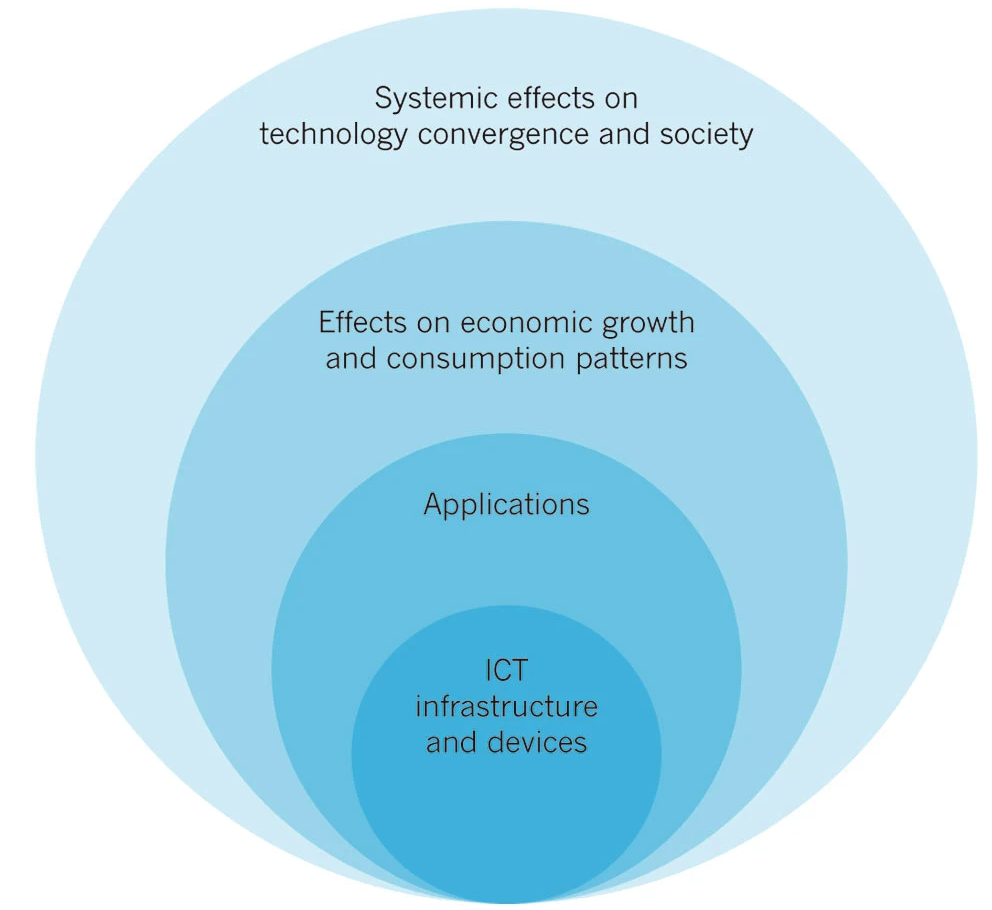
\includegraphics[width=.65 \textwidth]{./images/ICT_unintended_consequences.png}
    \centering
    \caption{Unintended consequences of ICT devices. The inner circle shows direct impacts of ICT equipment and infrastructure. The second circle represents applications of ICTs, such as remote working, machine learning algorithms and social media. The third circle refers to the effects on consumption and expectations caused by economic growth and changes in products. The outer circle represents larger societal and technological changes influenced by ICTs, including globalization, social movements, surveillance capitalism, interference with democratic elections, privacy and agency \cite{williams2011environmental}.}
    \label{ICT_unintended_consequences}
\end{figure}


%%%%%%%%%%%%%%%%%%%%% Surveillance Capitalism %%%%%%%%%%%%%%%%%%%%%%%%%%
\subsection{Surveillance Capitalism}
The rise of big data and advances in computing hardware (notably the graphical processing units (GPUs)) have led to the widespread advances and popularity in machine learning. While there are many beneficial applications to this, it has also ushered in a new era of \textit{surveillance capitalism}. This new economic order utilizes human experience as free raw material for a hidden commercial practice of extraction, prediction and sales \cite{zuboff2019surveillance}. Every day we generate 2.5 quintillion\footnote{1 quntillion bytes is equivalent to $10^{18}$ bytes} bytes of data \cite{forbes2018bigdata}. This consumer data is extracted from each computer mediated transaction, government institutions, emails, surveillance cameras, transportation services, social media, and the Internet of things (anything connected to the Internet from self driving cars to fitbits to smart fridges). A classic example of this is Google. By giving away free products and services, the company is able to harvest even more customer data.

Thanks to the advances in computing hardware, machine learning can now be applied to these enormous datasets to extract valuable customer information and patterns. This has a two-fold purpose: the company can generate revenue primarily by selling customized advertising, while the users get a free service and an “optimal” experience through tailored recommendations and content. In this model, people are no longer consumers (person purchases a product); instead they are users (person uses a product or service which harvests their data) \cite{zuboff2019surveillance}. While economical for many businesses, there are significant unintended consequences. By effectively monetizing likes, shares and time spent on a service, a global architecture of behavioural modifications has arisen through seeking behavioural certainty, predicting and manipulating behaviour, selling products and services and manipulating public opinion \cite{landwehr2019high}. This automated manipulation of behavior has resulted in addiction and a decline in mental health \cite{shakya2017association}, the undermining of the democratic process \cite{vaidhyanathan2018antisocial} and consumerism with its attendant environmental costs.

However, this increased surveillance and communication data presents a trade-off. On one hand, the data has helped both scientists, responders, and everyday citizens in the wake of natural disasters \cite{CNBC2020twitterclimatechange, moore2020using}. By augmenting existing emergency response structures, social media platforms have become an invaluable medium for communicating disaster preparation, food-security and recovery issues during these events \cite{moore2020using, CNBC2020twitterclimatechange, niles2019social}. On the other hand, this economic model has also led to a loss of privacy and supports surveillance conducted by both corporations and the state \cite{landwehr2019high}. Although protesters are using social media to spread, organize and document information, law enforcement agencies and the state are using social media data to track down protesters for prosecution \cite{owen2017monitoring}. This was evident in the 2020 George Floyd protests in the United States \cite{businessinsider2020georgefloyd}. 


% %%%%%%%%%%%%%%%%%%%%% Mental Health %%%%%%%%%%%%%%%%%%%%%%%%%%
% \subsection{Mental Health — From Persuasion to Addiction}
% Lecture 8

% In recent years we have seen a steep increase in social media usage (Figure \ref{Social_Media_Usage}).

% \begin{figure}[h]
%     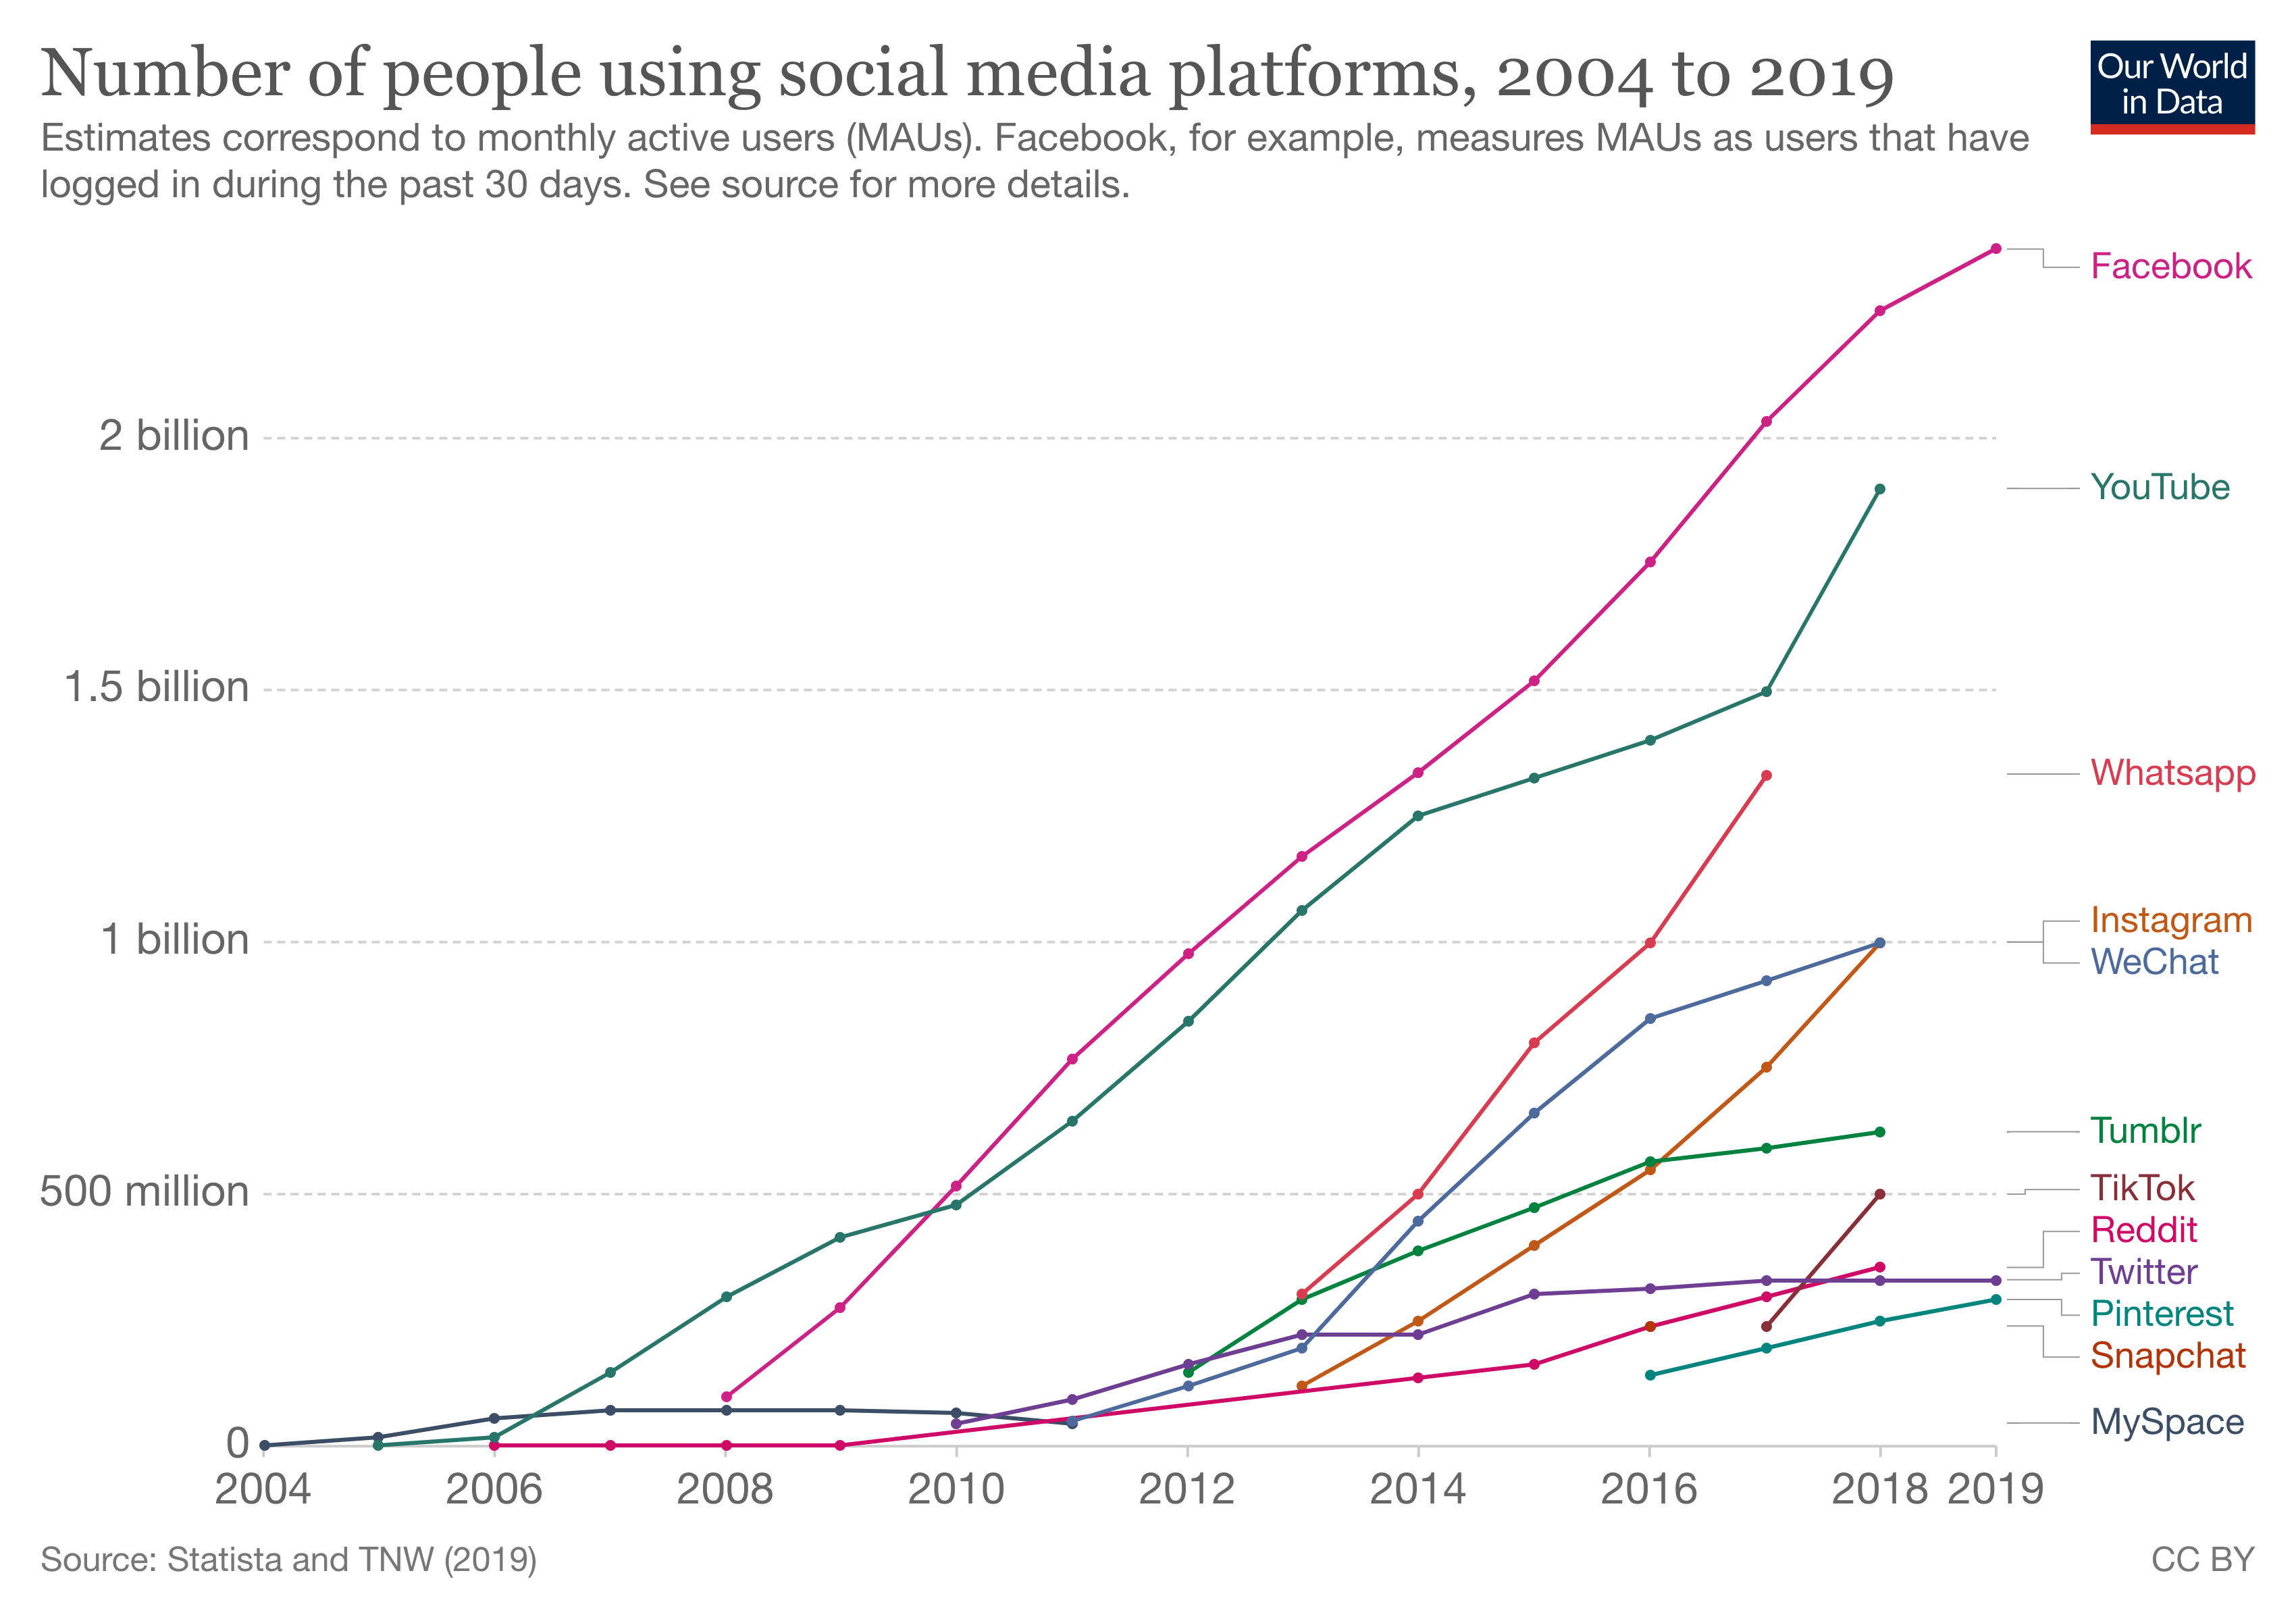
\includegraphics[width=.9 \textwidth]{./images/users-by-social-media-platform.png}
%     \centering
%     \caption{\textit{Number of people using social media platforms from 2004 to 2018 \cite{owidinternet}.}}
%     \label{Social_Media_Usage}
% \end{figure}


%%%%%%%%%%%%%%%%% Social Media & Social Movements %%%%%%%%%%%%%%%%%%%%%%
\subsection{Social Media as a Tool For Social Movements}
The media, including print, radio, television, and social media, have the ability to manipulate the capacity of citizen’s engagement in the public sphere \cite{lopes2014impact}. Social media is an unprecedented tool for generating new ways of interaction: not only are people able to view and use information, but they are able to directly express and discuss their thoughts and ideas on an interactive platform. Social media has taken off and there has been a steep increase in social media usage in recent years (Figure \ref{Social_Media_Usage}). While traditional forms of activism are still present, there has been a distinct shift towards using social media platforms with approximately 40\% of Americans engaging with social-political issues on digital platforms \cite{rainie2012social}. Users with higher levels of social media usage and a social network that includes individuals who support or participate in social movements tend to have a higher interest in participating in social movements \cite{hwang2015social}. As well, social media is a statistically significant predictor of protest activity \cite{lopes2014impact}. 

\begin{figure}[h]
    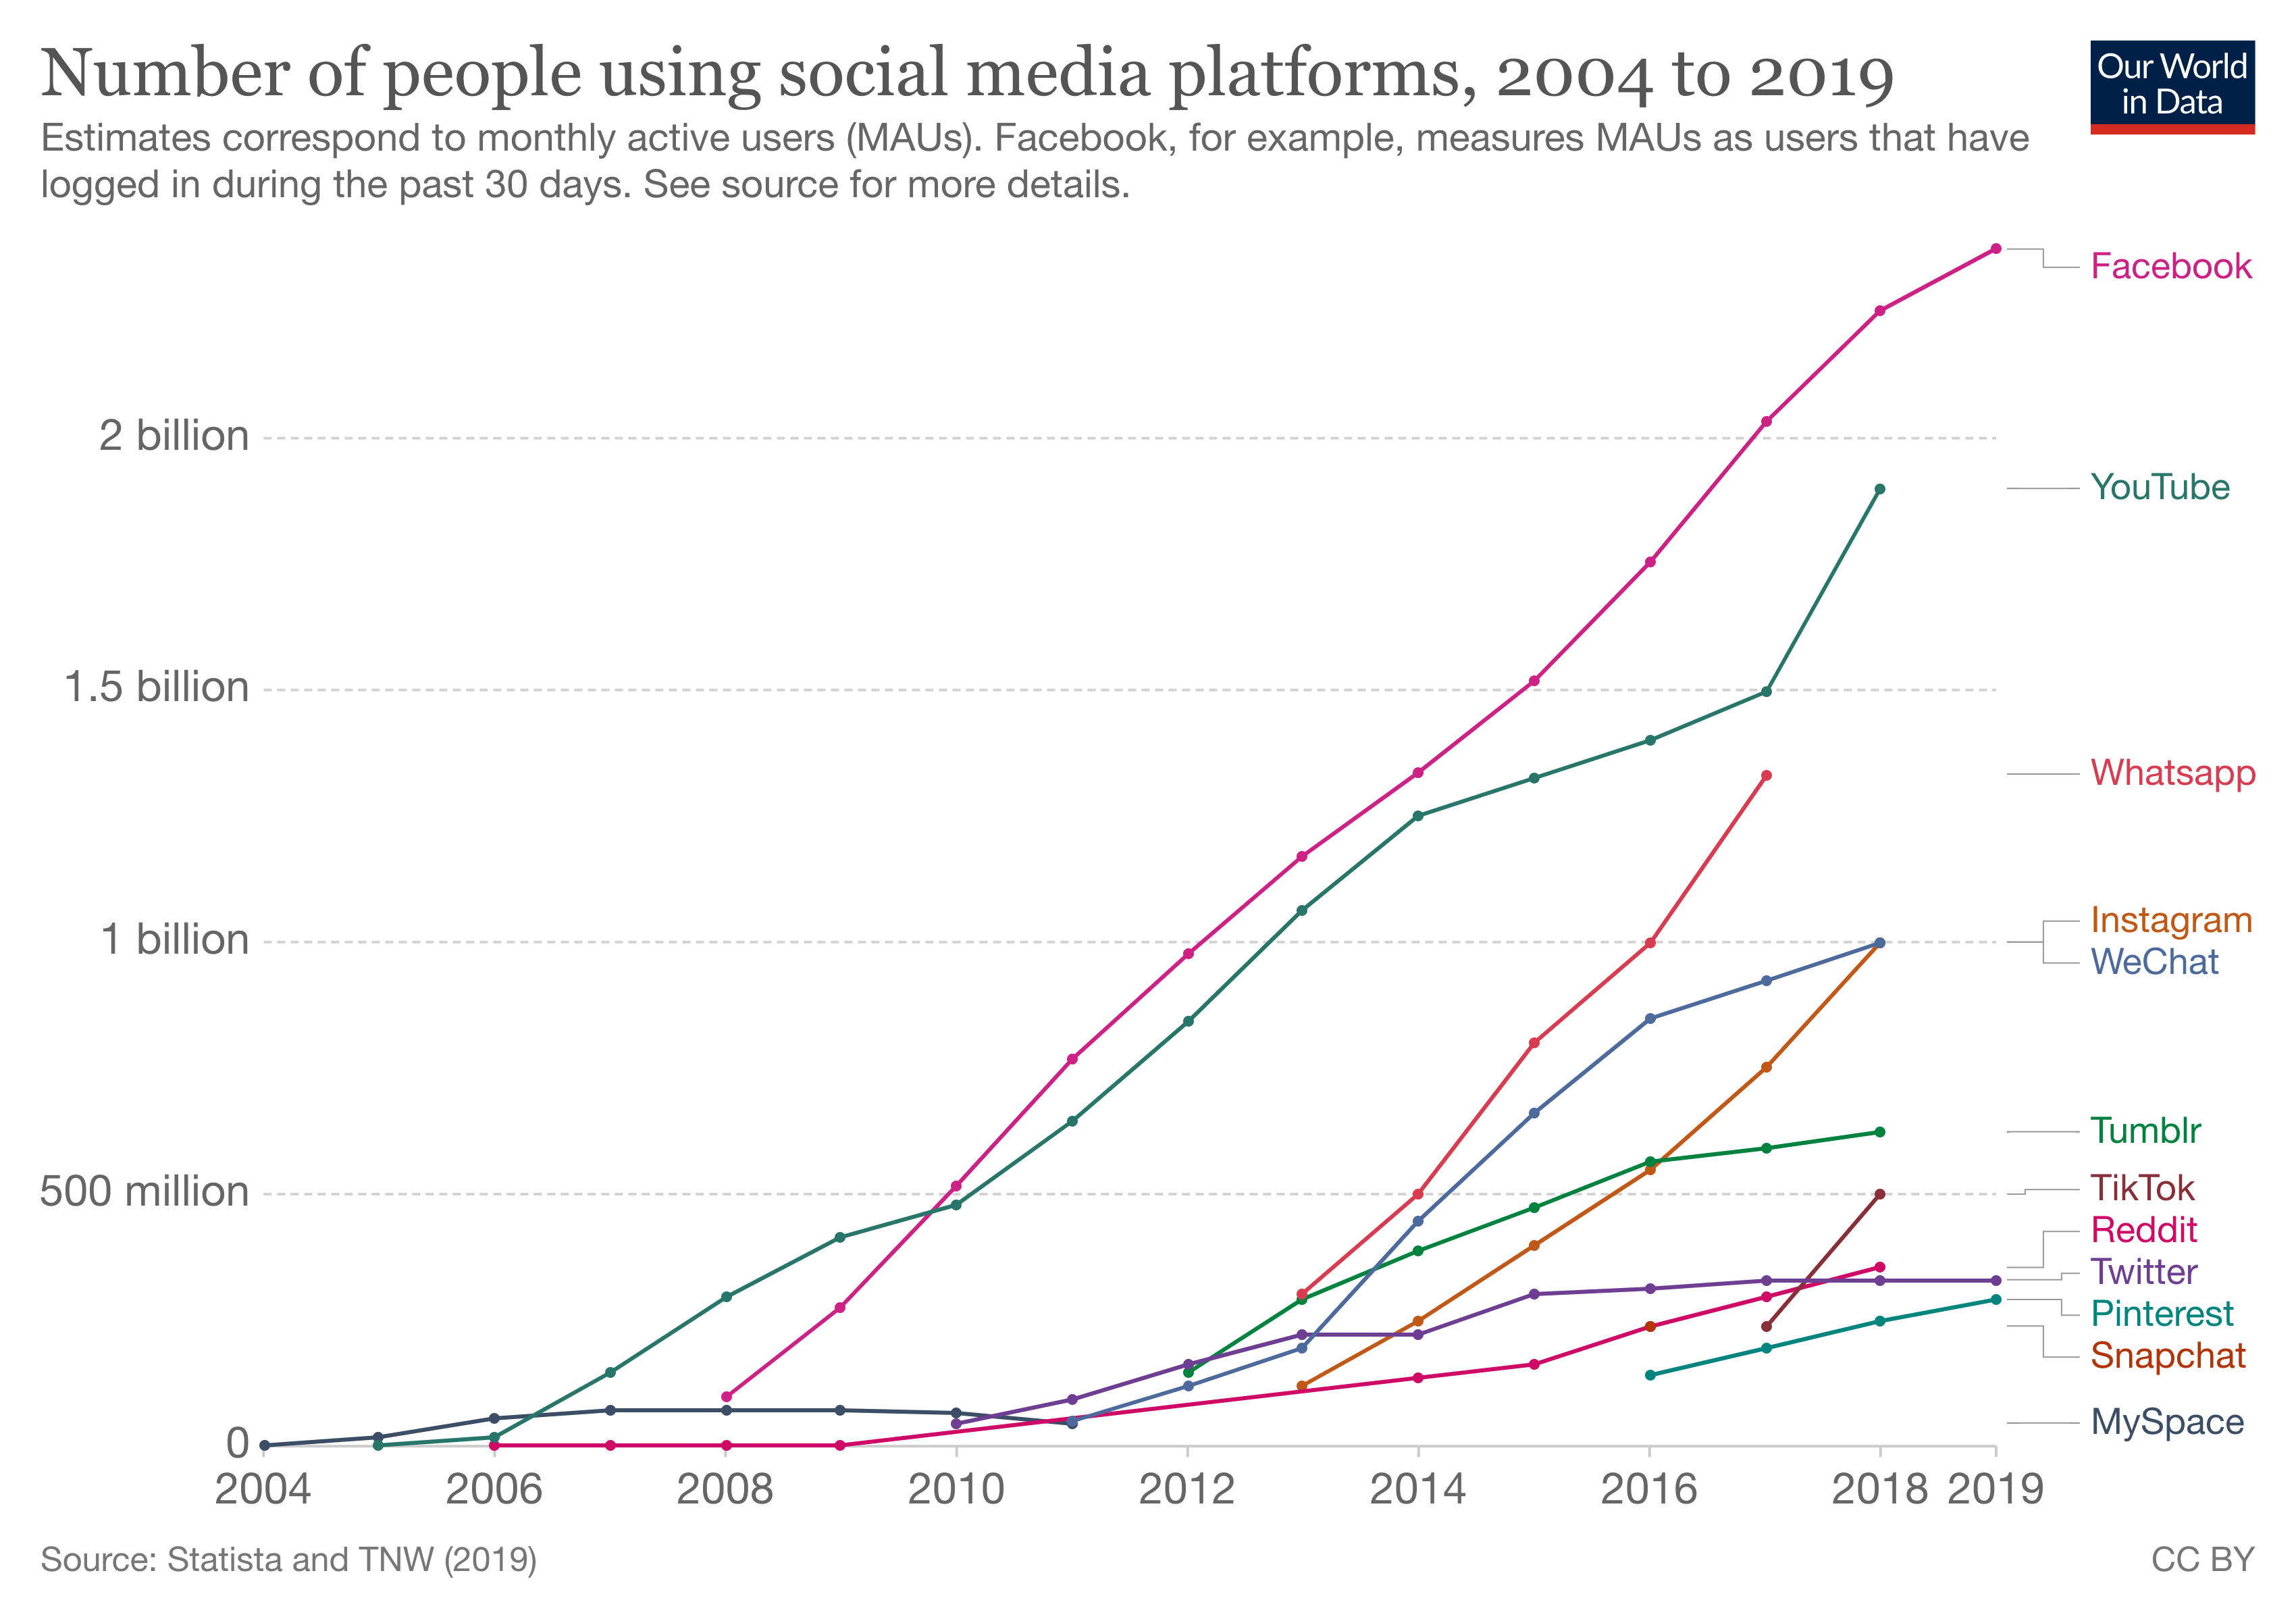
\includegraphics[width=.85 \textwidth]{./images/users-by-social-media-platform.png}
    \centering
    \caption{Number of people worldwide using social media platforms from 2004 to 2019 \cite{owidinternet}.}
    \label{Social_Media_Usage}
\end{figure}

Through this low friction communication, social media has made it easier to access and transmit information on social movements, to enlarge a base of supporters and to mobilize people to participate in social movements \cite{hwang2015social, mundt2018scaling}.  Social media can also be used to effectively mobilize funding through donations and crowd-funding campaigns \cite{sommerfeldt2013online, doan2018beyond}. Using social media to mobilize and coordinate support, the People's Climate Movement was reportedly the largest mass mobilization across the globe and it helped to reframe the online discourse on global climate change \cite{thorson2016climate}.

One catch of this groundswell of mobilization in online movements is \textit{slacktivism} within supporters. Slacktivism is low-grade virtual participation that allows supporters to feel a false sense of achievement, preventing them from further engagement with the movement. While defenders of slacktivism tend to argue that it supplements substantive actions, critiques of it are widespread (Figure \ref{slacktivism}). Rather than genuine commitment or engagement in efforts that bring about systemic change, the driving force of widespread liking, sharing or tweeting is often self-indulgent—a self-interested political engagement whose intention is to fulfill one’s personal desire to have a political impact or to boost one’s feelings of personal efficacy \cite{dennis2019beyond}.  As well, it may also reduce the number of supporters willing to engage with a movement offline \cite{mundt2018scaling}. While it is clear that social media and digital platforms offer social movements many opportunities, it is important for movements to also engage in more powerful or traditional forms of protest. 

\begin{figure}[h]
    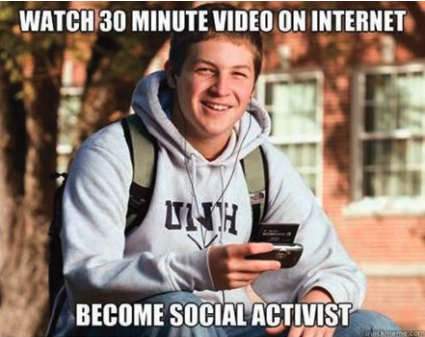
\includegraphics[width=.7 \textwidth]{./images/slacktivism.png}
    \centering
    \caption{A widely shared meme critiquing the slacktivism (Internet users that superficially support a cause while doing little to no effort) surrounding the 30-minute video \textit{Kony 2012} \cite{dennis2019beyond}. Ironically, the spread of this viral meme could also be considered a form of slacktivism.}
    \label{slacktivism}
\end{figure}

\subsubsection{The Climate Misinformation Movement}
Although social media is an effective tool for spreading information, it is poorly suited to the communication of a complex science. One of the earliest cases of this was Michael Mann’s publishing of the ``hockey stick" scientific study, wherein he reconstructed a 1,000 year temperature record that demonstrated a relatively flat downward period and a sudden uptick in temperature, resembling a hockey stick \cite{mann1999northern}. Despite the research within the landmark paper being replicated many times and receiving numerous awards, from the general public Mann has received death threats, postage contaminated with anthrax and was the subject of dozens of investigations spearheaded by politicians \cite{washingtonpost2016mann}. By nature, content on social media is fairly unregulated and does not distinguish between experts and non-experts. While the interest in environmental research may be helpful, the often unwarranted negative backlash erodes the signifiers of expertise, has minimal fact checking or accountability, and creates a system where experts are vastly outnumbered.

Social media also tends to latch on to single studies or specific incidents rather than syntheses. Also known as \textit{cherry picking}, this logical fallacy consists of intentionally selecting a data cluster or pattern to suit a particular argument \cite{logicalfallacies2021}. An unfortunate example of this is the climate myth being spread on social media platforms that global warming and sea level rise is a hoax because Antarctica is gaining ice. Sea ice forms around the continent in the winter months and it nearly completely melts in the summer; this annual cycle of growing and shrinking does not play a role in the rising or falling of sea levels. Whereas Antarctic land ice has accumulated over thousands of years through snowfall and it represents stored ocean water that once fell as precipitation. When this land ice melts it will return to the ocean, thereby raising the sea level. Despite the science showing that Antarctic land ice has lost substantial mass (Figure \ref{Antartica_sea_ice} left), online skeptics have instead cherry picked the slight increase in Antarctic sea ice (Figure \ref{Antartica_sea_ice} right), despite it being completely irrelevant to the discussion of sea level rise \cite{skepticalscientist2021antarticaice}. 

\begin{figure}[h]
    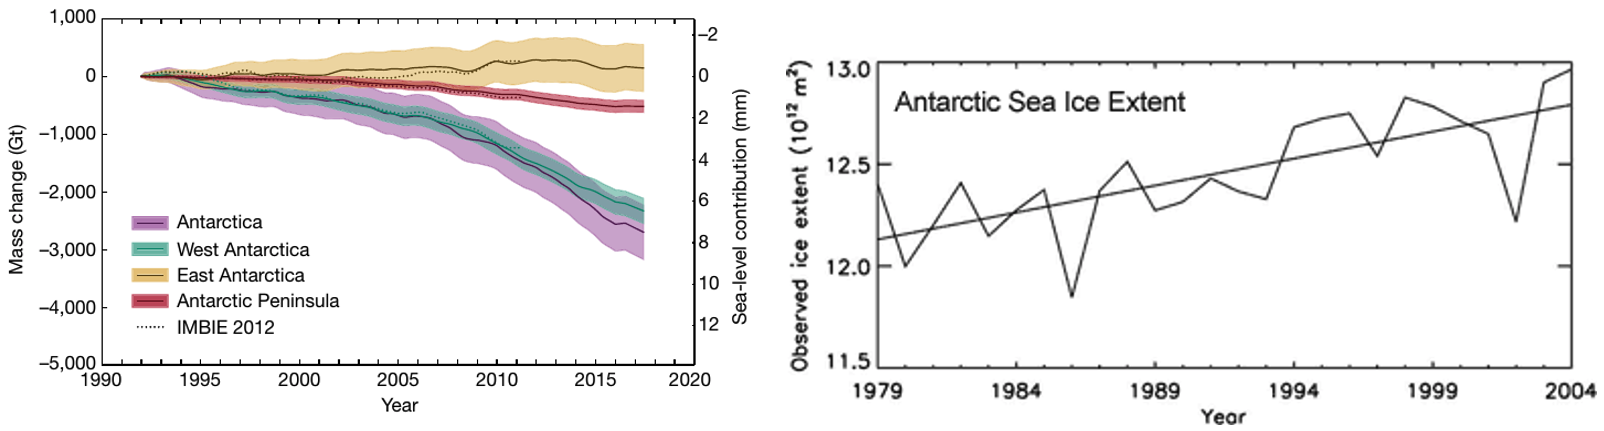
\includegraphics[width=.99 \textwidth]{./images/Antartica_sea_ice.png}
    \centering
    \caption{Change in mass of Antarctic ice. \textbf{(Left)} Overall, Antarctica land ice is rapidly decreasing (purple), however, there is geographical variation and East Antarctica (yellow) had a slight increase in mass \cite{shepherd2018mass}. \textbf{(Right)} For a period of time, Antarctica sea ice was increasing \cite{zhang2007increasing}. By cherry picking this slight decrease in Antarctic sea ice (or the modest increase in East Antarctica), online skeptics were able to spread the myth that Antarctica was gaining ice.}
    \label{Antartica_sea_ice}
\end{figure}

Social media also allows us to directly connect with people, ideas or groups we are interested in, which gives rise to a kind of social bias. Known as \textit{confirmation bias}, this cognitive bias means that people are more likely to seek out and agree with ideas that fit their preconception, while ignoring and dismissing information that is conflicting \cite{cognitivebias2021}. Social media thus creates echo chambers that allow people to only be exposed to information that confirms their existing beliefs, which has resulted in self-segregated and polarized online communities. This confirmation bias is then reinforced by the algorithms used to determine what people see online. These personalization technologies strive to present the most engaging and relevant content for each individual, but they also give rise to a plethora of algorithmic biases. These include the \textit{popularity bias} (promoting popular content irrespective to its quality), tailoring content and advertisements to individual users, and the \textit{filter bubble} (the more you click on a particular source, the more a social media will show you that site’s content). While there are benefits to this, it unfortunately isolates people from diverse perspectives thereby strengthening confirmation bias \cite{scientificamerican2018biassocialmedia}.

Since social media is a platform that facilitates freedom of expression and speech, it also allows users to exercise their right to voice their opinions while simultaneously silencing those they oppose. This can lead to a highly polarized environment that silences alternate or moderate voices; as well, opinions or science that are complex, nuanced or that does not belong to a dominant group are aggressively silenced \cite{lim2017freedom}. Also known as the \textit{spiral of silence theory}, those who perceive their opinion group as ascendant are more likely to express their opinions publicly; those who perceive their opinions to be in decline choose to silence themselves to avoid the threat of social sanctions, isolation and conflict. Often people are more frightened of social isolation and punishment than being wrong, so they join the masses even though they do not agree with them \cite{noelle1974spiral}. Although these phenomenons are not new, social media has simply enhanced these existing human and societal tendencies.

In addition to these cognitive and algorithmic biases making people vulnerable to misinformation spread, there is a well-funded campaign to frame climate change as a highly polarizing issue sowed with doubt. Between 2002 and 2010, \$118 million of dark money from anonymous billionaires (mostly fossil fuel sources) were distributed to 102 think tanks to cast doubt on the science behind climate change \cite{guardian2018darkmoney}. This affects the use of social media in building environmental movements, which are often at odds with the commercial and industrial players that can use social media platforms to influence how successfully a movement’s messages spread online. 


%%%%%%%%%%%%%%%%%%%%%%%% The Sharing Economy %%%%%%%%%%%%%%%%%%%%%%%%%%%
% \subsection{The Sharing Economy}
% Oct 27 lecture (transportation sector)

% \subsection{Commodification of Learning}
% lecture 1, slide 25
% chalk \& blackboard vs. all that crap today..

% \subsection{Positive Stuff}
% Nov 3 - Environmental Benefits


%%%%%%%%%%%%%%%%%%%%%%%%%%%%%%%%%%%%%%%%%%%%%%%%%%%%%%%%%%%%%%%%%%%%%%%%
%%%%%%%%%%%%%%%%%%%%%% Is The Internet Green? %%%%%%%%%%%%%%%%%%%%%%%%%%
%%%%%%%%%%%%%%%%%%%%%%%%%%%%%%%%%%%%%%%%%%%%%%%%%%%%%%%%%%%%%%%%%%%%%%%%
\cleardoublepage
\section{Is the Internet Green?} \label{SECTION_DISCUSSION}

In this journey together we have tried to answer this deceptively simple question. In doing so, it appears to be a complex question that cannot be answered: depending on the assumptions and boundaries that you choose, you might arrive to very different conclusions. As typical for infrastructures, we tend to take them for granted and they are often invisible until they stop working. The Internet is no exception. Also referred to as ultra-large scale systems (ULSS) \cite{northrop2006ultra}, this massive and complex infrastructure we know as the Internet is the result of a very large number of design decision over time. In our rush to solve environmental problems with digital technologies, we have forgotten the largely invisible footprint of the Internet itself; this physicality of the Internet is what we have tried to highlight with this paper.

In the simplest sense, we could compare the LCA of a few sectors when they use digital or non-digital medians. In the case of digital versus print, we find that digital options were better for books \cite{bull2014comparative}, newspapers \cite{moberg2010printed} and magazines \cite{ahmadi2015life}. When it came to teaching, however, using a printed textbook had a much lower impact than web based electronic teaching aids \cite{enroth2009environmental}. With regards to commercial activities, e-commerce may be better or worse depending on which future business scenario is realized \cite{caudill2000lifecycle}. Even though these studies answer the question in the most limited sense (for a very specific application using a variety of crucial assumptions in their methodology), this does not really address our big question. 

Although the ecological footprint (the environmental and social impacts of the processes that sustain us) is a powerful metric, we also need to examine the Internet's \textit{handprint}: the changes to the environmental and social impacts that we cause outside of our footprints. Whereas the footprint refers to the negative environmental impacts, the handprint can be used to refer to the positive impacts. For footprints we are trying to reduce them to zero; with a handprint there is no limit to the good that can be achieved \cite{gronman2019carbon}. A simple example to illustrate the handprint is the process I took to write this thesis. I wrote the first and last word of my thesis while living in the longest lockdown in North America\footnote{As of writing, my 5 month anniversary of continuous winter lockdown is today on April 23, 2021. The spring lockdown was fortunately shorter at only 129 days \cite{cfib2021torontolockdown}.}. I have not consulted a single physical book, newspaper or journal, worked inside a library, worked from my academic office, attended an in-person lecture or been to an in-person meeting with my supervisor since I started writing. And yet I have been able to complete my degree completely virtually: during just this winter lockdown, I have completed the coursework for my degree, taught a course, had (almost) weekly thesis meetings with my supervisor, consulted a plethora of online resources for my research and used a cloud computing service to compile the \LaTeX \; that I typesetted this thesis with. All of this from my tiny home desk without breaking any quarantine measures. Although the handprint is even more difficult to quantify than the footprint, a discussion of whether the Internet is green would be incomplete without it. While the footprint and unintended consequences of our ICT network is extensive and daunting, it is undeniable the good it has also done for our society.

So perhaps we have been asking the wrong question all along. Rather than asking whether the Internet is green, we should instead be asking a very different question: what can we do to make the Internet more green while simultaneously improving the good that it does?


%%%%%%%%%%%%%%%%%%%%%%%%%%%%%%%%%%%%%%%%%%%%%%%%%%%%%%%%%%%%%%%%%%%%%%%%
%%%%%%%%%%%%%%%%%%%%%%%%%%%% Bibliography %%%%%%%%%%%%%%%%%%%%%%%%%%%%%%
%%%%%%%%%%%%%%%%%%%%%%%%%%%%%%%%%%%%%%%%%%%%%%%%%%%%%%%%%%%%%%%%%%%%%%%%
\cleardoublepage
\bibliographystyle{acm}
\bibliography{references}

\end{document}


%%%%%%%%% References no room for %%%%%%%
%\cite{meadows2008thinking,walker2012resilience}

% Ursula M Franklin, The Real World of Technology \cite{franklin1999worldoftech}
% ``Technology, like democracy, includes ideas and practices; it includes myths and various models of reality. And like democracy, technology changes the social and individual relationships between us." (lecture 4, slide 47)

% Jenny Odell: How to Do Nothing \cite{odell2019doingnothing}